\documentclass[11pt,a4paper]{report}
\usepackage{amssymb,amsmath}
\usepackage{enumitem}
\setitemize{noitemsep,topsep=0pt,parsep=0pt,partopsep=0pt}

\usepackage{soul} % underlines
\setuldepth{aaaa}
\usepackage{framed}

%% enable markdown's stars to bold/italic sections of code -- requires lualatex!
\usepackage{luacode,luatexbase}
\begin{luacode}
   -- Use Lua captures to extract material affected by markdown
   function allstars (line) 
      line = string.gsub( line, "(%*%*%*)(.-)(%*%*%*)", "{\\bfseries\\itshape %2}")
      line = string.gsub( line, "(%*%*)(.-)(%*%*)", "{\\bfseries %2}" )
      line = string.gsub( line, "(%*)(.-)(%*)", "{\\itshape %2}" )
      return line
   end
\end{luacode}

\newcommand\markdownon{%
   \directlua{luatexbase.add_to_callback( "process_input_buffer", allstars, "allstars" )}}
\newcommand\markdownoff{%
   \directlua{luatexbase.remove_from_callback( "process_input_buffer", "allstars" )}}



%\usepackage[style=authoryear]{biblatex}
\usepackage[style=numeric,maxbibnames=19, maxcitenames=2,firstinits=true]{biblatex}
\addbibresource{biblio.bib}
\addbibresource{cogarch.bib}
\addbibresource{my-publications.bib}
\addbibresource{mutual-modelling.bib}

\usepackage{pdflscape}

\usepackage{fontspec}
\defaultfontfeatures{Ligatures=TeX,Scale=MatchLowercase}
\setmainfont[]{cantarell}

\usepackage{graphicx}
\graphicspath{{figs/}}
\usepackage{wrapfig}
\usepackage{hyperref}
\urlstyle{same}  % don't use monospace font for urls
\usepackage[margin=4pt]{subcaption}

\usepackage[a4paper,left=2cm,right=2cm,top=1.5cm,bottom=1.5cm]{geometry}
\usepackage{longtable,booktabs}

\usepackage{pgfgantt}
\usepackage{rotating}

\usepackage{tocloft}

\usepackage[compact]{titlesec}
\usepackage{blindtext, color}
\definecolor{gray75}{gray}{0.75}
\newcommand{\hsp}{\hspace{20pt}}
\titleformat{\chapter}[hang]{\LARGE\bfseries}{\hsp\textcolor{gray75}{|}\hsp}{0pt}{\LARGE\bfseries}

%\titlespacing*{\section}
%{0pt}{5.5ex plus 1ex minus .2ex}{4.3ex plus .2ex}
%\titlespacing*{\subsection}
%{0pt}{5.5ex plus 1ex minus .2ex}{4.3ex plus .2ex}


\renewcommand{\thesubsubsection}{}

\usepackage{xspace}
\newcommand{\project}{WizUs\xspace}

\newcommand{\task}[2]{\vspace{0.5cm}\noindent\emph{Task T#1}: {\bf #2}\par}

\newcommand{\D}[3]{\emph{Deliverable D#1} (M#2): #3\\}

\newcommand{\TODO}[1]{{\color{red}\textbf{TODO: #1}}}
%\newcommand{\TODO}[1]{}

\newcommand{\severin}[1]{{\color{red}\textbf{Severin: #1}}}
\newcommand{\toseverin}[1]{{\color{red}\textbf{To Severin: #1}}}
\newcommand{\eu}[1]{{\color{teal}\textbf{Guidelines EU ERC: #1}}}
%\newcommand{\eu}[1]{}
\newcommand{\cellgrey}{\cellcolor[gray]{0.85}}

\setcounter{secnumdepth}{0} % prevent section numbering, but still add sections to ToC

\title{\project - Part B}

\begin{document}
\markdownon
\maketitle

\begin{center}
    ERC Consolidator Grant 2020

    \vspace{2cm}
    
\includegraphics[width=0.7\linewidth]{logo}

    \textbf{\LARGE Socially-Driven Robots to Support Human-Human Interactions}

    \vspace{2cm}
    {\Huge \project}

\end{center}

    \vspace{2cm}

\begin{itemize}
    \item Principal Investigator: \textbf{Pr Séverin Lemaignan}
    \item Host institution: \textbf{University of the West of England, Bristol Robotics
        Laboratory}
    \item Duration: \textbf{60 months} (5 years)
\end{itemize}

\section*{Abstract}\label{abstract}

\eu{The abstract (summary) should, at a glance, provide the reader with a clear
understanding of the objectives of the research proposal and how they will be
achieved. The abstract will be used as the short description of your research
proposal in the evaluation process and in communications to contact in
particular the potential remote referees and/or inform the Commission and/or the
programme management committees and/or relevant national funding agencies
(provided you give permission to do so where requested in the online proposal
submission forms, section 1). It must therefore be short and precise and should
not contain confidential information. \\
Please use plain typed text, avoiding formulae and other special characters. The
abstract must be written in English. There is a limit of 2000 characters (spaces
and line breaks included).}


Knowlingly or not, AI is part of our daily life, from shopping suggestions, to
automated agents that respond our phone calls. Robots are coming next, to deliver
our parcels faster or support our ageing society. Many fears that these
technologies might isolate individuals, and exert further strain on our fragile
social fabric.

Does it have to be the case, though? Could instead a suitably-programmed robot
\textbf{enhance} social interactions between humans? Could social robots become
the tools to build stronger bonds and interactions within our societies? This
question is the backbone of the \project research project, and our specific
objective is that, \textbf{within 5 years, we create a socially-intelligent
robot, that (1) will have recognised social utility, and (2) will see long-term
acceptance by its end-users}.

We formulate two main hypotheses: (1) this objective can only be achieved if the
robot is \textbf{socially-driven}: the robot's behaviours must be driven by the
intention to support positive human-human interactions. How this general
principle translates into specific guidelines and algorithms -- while taking into
account the principles of a responsible AI -- is the central
contribution of Work Package 1.

(2) Long-term acceptance can only be achieved if the end-users are genuinely
involved at every step of the design process. To this end, \project introduces a novel
methodology involving 'public-in-the-loop' machine learning: the large scale
participation of end-users, over extended periods of time, to teach the robot how to
become a good and responsible social helper.

\project tests these two hypotheses with an ambitious work programme. It
includes basic research and conceptual framing; extensive, beyond-state-of-art, technical
developments; and an ambitious experimental programme, with a combined three years
of field deployment of social robots in public spaces.

\project will provide a lasting legacy, paving the way forward for a
better understanding of the design of socially-intelligent robots that are
socially useful and acceptable on the long-term: \project opens a \textbf{unique
window into the positive role social robots can play in our future societies}.

\newpage

%\tableofcontents

\pagebreak

%%%%%%%%%%%%%%%%%%%%%%%%%%%%%%%%%%%%%%%%%%%%%%%%%%%%%%%%%%%%%%%%%%%%%%%%%%%%%%%%%%%%%%%%
%%%%%%%%%%%%%%%%%%%%%%%%%%%%%%%%%%%%%%%%%%%%%%%%%%%%%%%%%%%%%%%%%%%%%%%%%%%%%%%%%%%%%%%%
%%%%%%%%%%%%%%%%%%%%%%%%%%%%%%%%%%%%%%%%%%%%%%%%%%%%%%%%%%%%%%%%%%%%%%%%%%%%%%%%%%%%%%%%
%% Names of the Work packages

\newcommand{\wpOne}{Framing robot-supported human-human interaction}
\newcommand{\wpOneShort}{Framing r-HHI}


\newcommand{\wpTwo}{Real-world Social Situation Assessment}
\newcommand{\wpTwoShort}{Social Situation Assessment}

\newcommand{\wpThree}{Trustworthy-by-design socio-cognitive architecture for robot-supported human-human interactions}
\newcommand{\wpThreeShort}{Socio-cognitive architecture}

\newcommand{\wpFour}{Data-driven social behaviour generation}
\newcommand{\wpFourShort}{Social behaviours}

\newcommand{\wpFive}{Evidence-based research: demonstrable usefulness of social robots in
real-world, complex scenarios}
\newcommand{\wpFiveShort}{Experimental investigation}

%\newcommand{\wpSeven}{TDB}
%\newcommand{\wpSevenShort}{TBD}

%\newcommand{\wpOne}{Project management \& dissemination}
%\newcommand{\wpOneShort}{\wpOne{}}




%%%%%%%%%%%%%%%%%%%%%%%%%%%%%%%%%%%%%%%%%%%%%%%%%%%%%%%%%%%%%%%%%%%%%%%%%%%%%%%%%%%%%%%

\newrefsection

%\textbf{B1.a. Extended Synopsis of the scientific proposal}

\TODO{impact/outcomes? -> explicitely state the high risk/high gain nature of
the project}

\TODO{discuss r-HHI more: what does it really mean to use a robot to support
HHI? link to responsible AI?}

\TODO{make sure everything in B1 is strongly grounded in litt}

\TODO{ensure the ethics side of things is solid}

\TODO{Notes papa:}
%\begin{itemize}
%    \item poser la question de la plus-value du robot social
%    \item presupposé: le robot peut faciliter les relations humaines -> donner
%        le contexte precis de pourquoi/ou/comment le robot peut aider
%    \item peut-on parler d'interaction au sens large?
%    \item question de l'intention: d'où vient l'intention du robot? -> l'idée
%        d'optimiser le nombre + qualité des interactions pas assez specifique
%    \item question de la mediation: fonction mediatrice du robot -> on peut
%        reformuler le projet en terme de: developper la base technologique
%        (robot) permettant à l'adulte/soignant/enseignant de se creer son outil
%        'ideal' de mediation, en le 'programmant' lui meme par demonstration
%    \item questions jurdiques: quelle est la responsabilité du robot?
%\end{itemize}

%\newpage 

\chapter{B1.a. Extended Synopsis of the scientific proposal}\label{part1}

\eu{(max 5 pages)}

\eu{The Extended Synopsis should give a concise presentation of the scientific
proposal, with particular attention to the ground-breaking nature of the
research project and the feasibility of the outlined scientific approach.
Describe the proposed work in the context of the state of the art of the field.
References to literature should also be included. References do not count
towards the page limits. It is important that this extended synopsis contains
all essential information including the feasibility of the scientific proposal
since the panel will only evaluate Part B1 at step 1.}

\section{Long-term vision and ground-breaking nature of the project}

The service and companion robots that we are set to interact with in the coming
years, are being designed and built today in labs and startups all over the
world. Can we however ensure 'by design' that they will have a net social utility?
\project \ul{defines} and \ul{implements} \textbf{a vision of AI
and social robotics that aims at placing the human at the centre of these
emerging technologies; supports stronger, more cohesive social interactions;
aims at reinforcing the social fabric of our societies rather than isolating
individuals}. \project seeks to answer the \textbf{why?} embedding social robots
in our society, and the \textbf{how?} to do so, from a technology and
`responsible AI' perspective.

This research is ground-breaking: \textbf{\project main objective is to design,
implement and demonstrate within 5 years the AI engine of a socially-intelligent
robot, that will result in a robot that (1) has an effective social utility, and
(2) will see long-term acceptance by its end-users}.

This objective is underpinned by two research hypotheses: (\textbf{H1}) for
end-users to ascribe social utility and engage with the robot over long periods
of time (months, years), the robot has to have its own long-term internal
motivation to be socially helpful -- a \emph{social teleology}. Libraries of
pre-programmed behaviours, as complex as they might be, are not sufficent.

(\textbf{H2}) Additionally, long-term acceptance can only be achieved if the
end-users are genuinely involved at every step of the design process, so that a
feeling of \emph{ownership} is fostered. We further hypothesise that
human-in-the-loop machine learning is the most effective way of generating
ownership, by enabling the design of robot behaviours that genuinely originate
from the end-users, and we therefore suggest that traditional human-in-the-loop
machine learning could and should be extended into 'public-in-the-loop' machine
learning, a new methodology to train a robot AI at scale, involving a large
range of stakeholders and end-users, in different interaction situations.



%How this general
%principle translates into specific guidelines and algorithms -- while taking into
%account the principles of a responsible AI -- is the central
%contribution of Work Package 1.

% This socially-driven goal forms what we call a \emph{social
%teleology}. its own goals have this objective can only be achieved if the
%robot is \textbf{socially-driven}: the robot's behaviours must be driven by the
%intention to support positive human-human interactions. 

\begin{wrapfigure}{r}{0.4\linewidth}
    \centering
    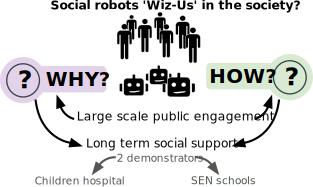
\includegraphics[width=0.9\linewidth]{concept}
    \label{fig|concept}
\end{wrapfigure}


The investigation of these hypotheses in \project is underpinned by the novel
idea of \textbf{robot-supported human-human interactions}, which reverses the
traditionally accepted, technology-centric, view on human-robot interactions.
Instead of having the robot at the centre of the stage, the humans are: we build
from pre-existing social interactions between people, and investigate where,
when and how robots could facilitate and enrich them. To this end, we will
deploy the \project robot for a year in a public space (the Bristol Science
museum, WeTheCurious), asking visitors to 'take control' of the robot for a
period of time, and use it to mediate interactions between other visitors of the
museum.  At the end of this experiment, we expect thousand of people to have had
experienced how robots could interact with human, and each of these experiences
will contribute to uncovering the basic principles of social interaction for
robots. This work is the focus of WP1.

While most of the interactions in the museum will be short-lived, two further
large scale experiments will take place over the course of the project: a
one-year experiment at the Bristol's children hospital, where the robot will
join one of the wards for children with long-term conditions, and engage the
children in playful social activities; another one-year experiment in one of
Bristol's Special Education Need (SEN) school, helping children with
psycho-social impairements to develop their social skills. In both these
experiments, the robot behaviours will be co-designed with, and learnt from the
end-users themselves: nurses, teachers, parents, and the children themselves.


\begin{wrapfigure}{l}{0.15\linewidth}
    \centering
    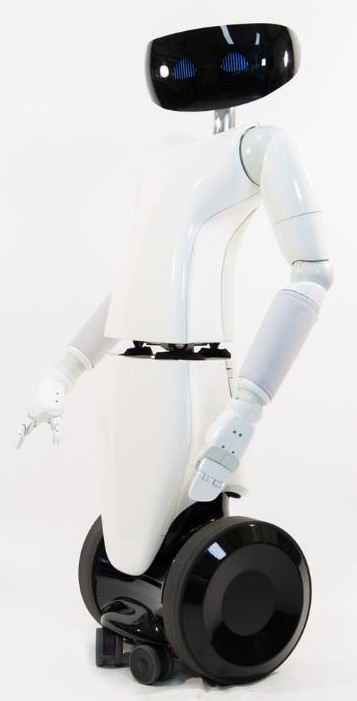
\includegraphics[width=\linewidth]{R1-profile}
    \label{fig|R1}
\end{wrapfigure}

Importantly, \project focuses specifically on the AI engine of the robot: I will
use an existing robotic platform (IIT's R1, left) and develop and train the
algorithms required to achieve autonomy and long-term social utility. After the
initial training period, the robot will indeed be \emph{autonomous}: while the
users will be provided tools to override the robot decisions at any time (via
both an app and touch sensors on the robot itself), it will otherwise
move and act on its own, without the need for constant supervision. To this end,
the robot will have ground-breaking perception and modelling capabilities (the
focus of WP2) to represent the current social situation, coupled with an
innovative cognitive architecture designed to combine internal social
drives with domain-specific action policies learnt from the end-users.

The robot actions themselves are designed to be limited to motions and
non-verbal communication mechanisms: non-verbal utterances using sounds, gaze,
joint attention, expressive motions. My team will in addition create a novel
non-verbal modality based on \emph{soundscapes}: sound landscapes that the robot
can modulate to influence the mood of the social environment (calm, excited,
worried, etc.).

Finally, \project is also about asserting and reinforcing the European
leadership in AI and intelligent robotics, in line with EU strong societal values: a
socially responsible AI, that guarantees, by design, long-term benefits to the
society. This requires leading major technological advances; leading the
development of the conceptual framework around socially intelligent robots that
we need to inform future policy making; and a strong leadership to meaningfully involve
the public at large in the design of these technologies. Through its objectives
and methodology, \textbf{\project will have a major contribution to building
this capacity in Europe}. 

\begin{framed}

\bf Over the 5 years of the fellowship, the
\project project will design and deliver a ground-breaking embodied AI for
socially intelligent robots. This AI will be responsible 'by design', have
demonstrable social utility and ensure long-term acceptance by end-users.
Co-developed with a large public using a novel methodology ('public-in-the-loop'
machine learning), its utility will be demonstrated over two one-year-long experiments in
socially sensitive environments.

\end{framed}

\section{Feasibility of the \project work programme}

Socially intelligent robots require unique, beyond state-of-the-art,
capabilities to \emph{(1)} understand the social interactions (social
situation awareness), \emph{(2)} autonomously decide the best course of action for
short-term and longer-term social influence, and \emph{(3)} perform the
appropriate social actions and exert said influence in an appropriate,
responsible manner.
However, extreme complexity hides behind these seemingly well-delineated steps:
not only the required technology is itself beyond state-of-the-art, but the
interplay between technology, socio-cognitive psychology, privacy and ethics is
only starting to be researched and understood. \project offers an
strong vision and an ambitious, evidenced-based, methodology to significantly
advance our understanding of this problem.

Over the course of 5 years, I will specifically investigate hypotheses H1 and H2
through the following research questions:

\begin{itemize}
    \item \textbf{R1} [conceptual framing]: what are the basic principles of
        responsible social interactions, that must form the foundations of a
        socially useful robot, accepted and used on the long run? What should
        motivate the robot to step in and attempt to help? What are the
        determinants and parameters of a social intervention, performed by a
        socially-driven robot, to support positive human-human social
        interactions? How to balance social utility and social responsibility?

    \item \textbf{R2} [implementation level]: how do these principles
        can be integrated into a principled, socially-driven teleological
        architecture for autonomous robots? How this should be combined with
        bottom-up action policies, designed and learnt from the end-users? How
        can we ensure 'by design' that the resulting AI will generate useful yet
        responsible, trustworthy, human-centered robot behaviour?

    \item \textbf{R3} [technology level]: where are the technological gaps in
        artificial social modeling and cognition, that prevent the actual
        realisation of a robot capable of effective social support, sustained
        over long period of time? How can we fill them?

    \item \textbf{R4} [experimental level]: can we demonstrate in complex, real
        world conditions, the effectiveness and usefulness of the
        robot-supported human-human interaction paradigm? Can we do so by
        involving the end-users at every stage of the design, implementation and
        testing cycle?

\end{itemize}


These research questions are addressed across five work-packages: \textbf{WP1}
is dedicated to the conceptual framing of the project (R1); \textbf{WP2} builds
on the principles identified in WP1, and translates them into socio-cognitive
representations and capabilities, identifying and filling the gaps in the
state-of-the-art (R3); in parallel to WP2, \textbf{WP3} transposes the
conceptual framework of WP1 into a principled cognitive architecture and
integrates together the cognitive functions of WP2 (R2); \textbf{WP4} looks at
how social robots can perform effective social interventions to exert positive
social influence (R3); and \textbf{WP5} organises the experimental fieldwork
that demonstrates the \project approach in ambitious and
complementary real-world situations (R4).

\subsection{WP1: \textbf{\wpOne}}

\noindent\framebox[\linewidth]{Duration: \textbf{Y1-Y3}; one senior post-doc
with background in sociology of technology}

The basic ambition of \project is to create a conceptual framework around social
robots in the human society, by re-framing the tradionally accepted idea of
\emph{human-robot interaction} into the human-centered idea of
\emph{robot-supported human-human interactions} (r-HHI): the robot is considered
from the perspective of how it can \emph{support} humans, and in particular,
support stronger, positive interactions between humans.

\textbf{T1.1 -- Conceptual framing of r-HHI} The first task in WP1 is to research and
define such a framework that will provide the (currently missing) conceptual
frame around questions like: what role for social robots? where to set the
boundaries of artificial social interactions? what does 'ethical-by-design',
'responsible-by-design' might mean in the context of social human-robot
interactions? 

In order to anchor T1.1 into the reality and complexity of human social
interactions, and to also involve the civil society in this framing process, the
task will embed \project into the 'City lab' experiment, conducted by Bristol's
science museum WeTheCurious. WeTheCurious is leading the push for a new form of
public engagement, call 'City Lab', that sees the visitors engaging in the
actual production of science. We will integrate \project in the City Lab to
co-design and co-produce robot-supported social interactions with the general
public. For an initial period of one year (Y2-Y3), one \project robot will be
permanently based at the museum.  Participants (children and adults) will be
guided, with the help of museum staff and a dedicated interface, into
teleoperating the robots to make them good 'social helpers'. This will generate
the quantitative and qualitative data to inform questions like 'what role for
the robot?', 'when to intervene?', 'what are the effective and acceptable social
influence techniques?'. It will also be a unique example of large-scale
participatory design with future end-users of social robots.

\textbf{Specific resources} I have an on-going collaboration with WeTheCurious,
and preliminary meetings were held to discuss specific requirements for the
\project project. The museum is committed to the project, and will include
\project in its official programme of activities.

%%%%%%%%%%%%%%%%%%%%%%%%%%%%%%%%%%%%%%%%%%%%%%%%%%%%%%%%%%%%%%%%%%%%%%%%%%%%%%%
% WeTheCurious
% 
% - one robot completelty controlled by children, one by adults
% 
% what to learn?
% 
% - when to approach? when to prompt? [example of the salesman/museum facilitator]
% - when is the right time to help/intervene or not? 'child being told off by
% parents -> not the right time!'
% - group interactions -> when to intervene? what about peer-pressure? eg what if
% I tell off one child in front of another?
% - break the barrier for participation. Japanese Journal paper -> facilitating students questions
% - impact on moral norms? what behaviours is acceptable?
% - what role for the robot? another mediator? a peer?
% - what can we do with that 'alien creature'
% 
% - robot taking one child to talk to the museum mediators ("I, robot, am  shy!
% would you come with me?")
% 
% - learning how to adjust behaviour based on personality
% - 'why do I behave like that with that person, and like this with that other
% person?'
% 
% - reinforcement learning instead of human-in-the-loop -> what reinforcement
% signal? engagement
% 
% - the robot that 'take sides': take side against the adults? -> bending in its
% role?
% 
% 
% - social embarassment
% - space for pretence: the robot can adopt an 'artificial role' as long as it is
% possible (accpetable/...) to pretend the robot is



\textbf{T1.2 -- Determinants and principles of robot-supported social
interactions} The conceptual framework identified in T1.1 is translated
into a set of \emph{interaction design principles}, \emph{determinants} and
\emph{parameters} that will together form a set of requirements and objectives
for the socio-cognitive capabilities and architecture developed in WP2 and WP3.

\subsection{WP2: \textbf{\wpTwo}}

\noindent\framebox[\linewidth]{Duration: \textbf{Y1-Y4}; one post-doc in social
signal processing/machine learning/cognitive modelling}

In WP2, the project addresses the key scientific and technical pre-requisites to
effectively deliver WP3's architecture:  the scientific understanding and
formalisation of the \emph{social fabric} in which the robot is embedded, in its
full complexity: spatial characteristics (proxemics; group dynamics; complex,
dynamic attentional mechanisms); psycho-social determinants (social roles and
hierarchies; social groups; mental modelling; anthropomorphic ascriptions);
temporal characteristics (effects of novelty; dynamics of anthropomorphism and
mental ascriptions; group dynamics).  While several of these capabilities have
been previously investigated is isolation~\cite{lemaignan2014dynamics,
flook2019impact,lemaignan2015youre, fink2014which, ros2010which,
warnier2012when, lemaignan2015mutual, dillenbourg2016symmetry,
winkle2019effective}, this WP will deliver the first complete and integrated
model of artificial cognition that account for social interactions in their full
extend, significantly extending the state-of-art~\cite{lemaignan2017artificial,
baxter2016cognitive}.


\textbf{T2.1 -- Hybrid situation assessment and knowledge representation}
Knowledge representation and grounding is a fundamental building block for
cognitive architectures~\cite{lemaignan2017artificial,beetz2010cram}. This task
builds on existing state-of-art in knowledge representation and situation
assessment (eg~\cite{citeneeded}) and creates a coherent system of
representations for the cognitive architecture that extends the \sc{underworlds}
spatio-temporal representation tool developped by the
PI~\cite{lemaignan2018underworlds,sallami2019simulation} with knowledge
representation capabilities, using both established symbolic techniques (like
ontologies and first-order logic~\cite{lemaignan2010oro, tenorth2009knowrob}),
and hybrid symbolic/sub-symbolic modelling (using Jaeger's
conceptors~\cite{jaeger2014controlling}) as a new route to overcome the symbolic
grounding problem~\cite{harnad1990symbol}.

\textbf{T2.2 -- Social dynamics} This task focuses on the processing and
modelling of social signals, extending existing techniques, both model-based
(eg~\cite{lemaignan2016realtime,others}) and machine-learning based
(eg~\cite{chetouani,others}) This task goes beyond the state-of-the-art by
looking specifically at resolving highly dynamical signals (like gaze saccades
and micro facial expressions). While playing an fundamental role in social
interactions~\cite{citeneeded}, they are currently not investigated in social
robotics -- even though the technology (high speed cameras and embedded GPUs) to
achieve real-time classification of such cues is available.

\textbf{T2.3 -- Interaction and group dynamics} Building on T2.2, T2.3
investigates the automatic understanding and modelling of group-level social
interactions, like inter-personal affordances~\cite{pandey2013affordance}. It
includes spatial determinants (proxemics; group-level attention tracking);
psycho-social determinants (social roles and hierarchies; social groups) and
dynamics (effects of novelty; dynamics of anthropomorphism and mental
ascriptions; group dynamics). 


\textbf{T2.4 -- Social situation assessment} The integration of the social cues
from T2.2 and T2.3 results in a socio-cognitive model of the social environment
of the robot that we term \emph{social situation assessment}.  It effectively
extends the representation capabilities of T2.1 to the social sphere, and covers
the development of a complete social assessment pipeline, from social signal
perception (like automatic attention tracking, face recognition, sound
localisation, etc.) to higher-level socio-cognitive constructs, including group
dynamics and theory of mind (as I previously framed
in~\cite{lemaignan2015mutual, dillenbourg2016symmetry}). A focused experimental
programme accompanies T2.4, to demonstrate (in relative isolation) the resulting
socio-cognitive capabilties. In particular, the protocols identified by Frith
and Happé~\cite{frith1994autism} to investigate theory of mind with autistic
children offers an excellent experimental framework for social
robotics~\cite{lemaignan2015mutual} and will be employed.

\subsection{WP3: \textbf{\wpThree}}

\noindent\framebox[\linewidth]{Duration: \textbf{Y1-Y4}; one senior post-doc in
cognitive robotics; one PhD student}

This part of the programme is the technical core of the project: we will create a
novel socio-cognitive architecture for the robots, bringing together advanced
perception of the human social dynamics, intrinsic motivation to support human
interactions, and human-in-the-loop machine learning to create transparent,
trustworthy action policies. This WP is high-risk/high-gain, as no such combined
approach has been successfully implemented and deployed in real-world, complex
social situations. I mitigate the risk by ensuring cognitive functions are
decoupled from each other where sensible, and in particular, by ensuring that
the robot actions are generated independently through both an intrinsic
motivation mechanism, and a human-taught machine learning action policy, hence
creating a level of cognitive redundancy (with the corresponding arbitration
mechanisms in place where necessary).


\textbf{T3.1 -- Socially-driven architecture for long-term interaction} The
socio-cognitive architecture of \project robots builds from the principles (the
`why's?') identified in T1.3, and relies on a combination of socially-driven
intrinsic motivation (a \emph{social teleology}, T3.2), and human-in-the-loop machine
learning (T3.3) to progressively learn an social policy enabling long-term
autonomy. This task focuses on `bringing the pieces together' in a principled
manner.

We will specifically look at the requirement for \emph{long term} autonomy: Over
the last two years, we have observed an significant increase of studies
involving social robots, deployed in real-world settings (schools, care centres)
over relatively long periods of time (up to 2 or 3 months at a
time)~\cite{kunze2018artificial,leite2013social}, with some promissing results
in well defined situations, with pre-defined tasks (for example, learning
tasks~\cite{senft2019teaching}, or 'butler' in a social care
facility~\cite{hawes2017strands}). More generic (long-term) social autonomy
however requires additional, beyond-state-of-art research to (1) add a
\emph{social motivation} mechanism able to drive the robot's intentions over
time. This is specifically investigated in T3.2 and T3.3 below; (2) a level of
cognitive redundancy to ensure reliable perception and behaviour generation
(addressed by this task, with a dependency on the cognitive functions developped
in WP2 and WP4).

\textbf{T3.2 -- A social teleology for robots}
The case for \emph{teleological} (ie goal-driven) robotic architectures has been made in
the past~\cite{wrede2012towards}, but only effectively realised for relatively
simple cognitive systems (like curiosity-driven robot
animals~\cite{oudeyer2005playground} or motor babbling in infant-like
robots~\cite{forestier2017unified}). Socially-driven robots, participating in
complex interactions with humans, have been barely investigated. This task
covers the overall design of the architecture.


\textbf{T3.3 -- Learning from humans to achieve 'by-design' responsible \&
trustworthy AI} Building on my recent, promising results on human-in-the-loop
social learning~\cite{senft2017supervised,senft2019teaching,winkle2020coach}, this task
implements the learning mechanics (including the critical aspect of the
interface with the human teacher) to allow human participants to progressively
teach the robot a social policy to become a good social helper.

Additionally, a critical aspect of task T3.3 is to develop the arbitration
mechanism that combines the robot's social teleology (T3.2) with the human-taught
action policy. This arbitration mechanism will build on research on
reinforcement learning for experience transfer~\cite{madden2004transfer} that
enables the re-assessement of a policy (here, our intrisic motivation) based on
previous experience (here, the human-taught policy).

Finally, this task researches how human-in-the-loop machine learning enables a more
trustworthy AI system, by involving the end-users in the creation of the robot
behaviours, guaranteeing a level of behavioural transparency for the end-users.


\subsection{WP4: \textbf{\wpFour}} 

\noindent\framebox[\linewidth]{Duration: \textbf{Y2-Y5}; one post-doc in HRI/machine learning/learning from
demonstration}

Mirroring WP2's focus on understanding the social interactions, WP4 addresses the
question of social behaviour \emph{generation}: how to create natural
behaviours, engaging over a sustained period of time (eg not simply picking
scripted behaviours from a library, that are rapidly perceived as repetitive).

Using cloud-based speech recognition, the robots will be able to understand and
record the textual transcription of the what the end-users say (in WP5, mostly
children). The robots themselves are however purposefully designed \emph{not} to
speak, using instead non-verbal communication mechanisms (non-verbal utterances
using sounds, gaze, joint attention, expressive motions, etc). This is a
critical interaction design choice, that ensures we can more effectively manage
what cognitive capabilities are ascribed to the robot by the users (expectation
management).  \project seeks however to significantly push forward the
state-of-art of behaviour generation for robots, both in term of technique to
generate the behaviours, and in term of the nature of the non-verbal behaviours.

\textbf{T4.1 -- Behavioural baseline} T4.1 establishes a baseline for behaviour
generation, by surveying and implementing the current state of the art. In
addition to traditional approaches like behaviour libraries, this will cover
techniques like curiosity-driven behaviours~\cite{oudeyer2005playground},
Learning from Demonstration~\cite{billard2008robot, argall2009survey},
human-in-the-loop action policy learning~\cite{senft2016sparc,
senft2019teaching}. This baseline will enable early in-situ experimental
deployments (WP5), while also provide a comparison point for T4.2.

\textbf{T4.2 -- Machine learning for continuous motion generation} \project aims
at significantly advancing the state of the art in this regard, by combining two
existing techniques: (1) data-driven, continuous approach to behaviour
generation inspired by Learning from Demonstration; (2) interactive machine
learning in high-dimensional input/output spaces~\cite{senft2020woz}, where I
have shown with my students promising results for generating complex social
behaviours~\cite{senft2019teaching, winkle2020coach} that fully involve the
end-users~\cite{winkle2020methodology}.  By combining the two, I target
a breakthrough in robots' social behaviours generation: the generation of
non-repetitive, socially congruent and transparent social behaviours (including
gestures and gazes).

\textbf{T4.3 -- Non-verbal behaviours and robot soundscape} In task T4.3, we
introduce a novel non-verbal interaction modality for robots, based on
soundscapes: soundscapes are about creating a sound environment that reflects a
particular situation; they also have been shown to be an effective intervention
technique in the context special need treatments
(eg~\cite{greher2010soundscape}). The soundscapes that we will create, are
`owned' by the robot, and it can manipulate it itself, eg to create an
approachable, non-threatening, non-judgmental, social interaction context, or to
the establish the interaction into a trusted physical and emotional safe-space
for the children.

\textbf{Specific resource}: these soundscapes will be co-designed with Dr.
Dave Meckin, an expert on sound design for vulnerable children, who also works
at the host institution.

\subsection{WP5: \textbf{\wpFive}}

\noindent\framebox[\linewidth]{Duration: \textbf{Y2-Y5}; one post-doc (shared
with WP3)}

WP5 aims at convincingly demonstrating the importance and positive impact that
socially-driven, socially-responsible robotics may have. The experimental work
of \project will be organised around two ambitious long-term studies (in
addition to the museum study, T1.2), in complex, real-world environments: a
network of special needs schools, and the Bristol Children Hospital.

These environments also put the project in the unique position of actually
delivering high societal impact: besides the thousands of people that will
contribute to the design of the system at the museum, we anticipate 30+
hospitalised children with long-term conditions, and about 350\TODO{check with
Nigel} SEN-educated children to directly benefit from the project, showing how
robots can have a lasting, strong, positive impact on the society, also
establishing the idea of robots \ul{supporting} human interactions instead of
dehumanising our social relationships.


\textbf{T5.1 -- creation and deployment of a robot companion to
support physical and mental well-being, as well as foster social interactions,
in SEN schools} This task aims at demonstrating robot-supported social
interventions within the eco-system of SEN (Special Educational Needs)
schools. The aim is to effectively support the day-to-day work of the
school staff to support the development, learning and well-being of the
children. A \project robot will be deployed for one year (Y3) in a
Bristol-based SEN school (to be possibly extended to additional schools) to
investigate how an autonomous social robot can help shaping a spatial and social
school ecology that fosters mental well-being, while effectively supporting
student-student and student-teacher social interactions. The
robot behaviours will be co-designed with the teachers, the students, and the
parents through several preliminary design workshops

\textbf{Specific resources} this task will take place within a network of
Bristol-based SEN schools, with which I already have on-going collaborations
(child-robot interaction for children with autism at Bristol's Mendip School).
The task will be jointly supervised with local colleague and expert Dr.Nigel Newbutt,
who has a long track record of working with special needs schools.


\textbf{T5.2 -- creation and deployment of a small robot companion to support
isolated children during their hospital stay}, fully integrated and aware of the
wider hospital ecosystem. Over the course of this second, one-year long (Y4)
experiment, we will deploy one \project robot at the Bristol Children Hospital.
Using a \emph{mutual shaping} approach~\cite{winkle2018social} to design the
role of the robot with the different stakeholders (nurses, doctors, parents,
children), we will experimentally investigate how a social robot can support
hospitalised children with long-term conditions. The robot's role will revolve
around facilitating social interactions between possibly socially isolated
children, by fostering playful interaction with a yard.

\textbf{Specific resources} this task will take place at the Bristol Children
Hospital. Several preparatory meetings already took place with the head of the
hospital education service J. Bowyer, who will support the project, giving me
access to two of the long-term conditions wards for the duration of the studies.



\subsection{Capacity of the Principal Investigator to deliver on the work programme}

The project's ambitious scientific and technical goals are expected to deliver
major scientific, societal and technical impact, that extends beyond the end of
the fellowship. At the end of the fellowship, the PI is expected to be a
world-leader in the emerging field of socially-driven, responsible autonomous
service \& companion robots, building up the European capacity in this critical
field, that will have high societal and economical impact on several key sectors
like assistive technologies, entrainment, advanced manufacturing.

Pr. Lemaignan is in a unique position to deliver on the \project work plan.  He
has already established international recognition in human-robot interaction and
has likewise demonstrated strong leadership by leading research teams in three
different institutions (see Sections B1.b and B1.c below). Importantly, as
illustrated in Table~\ref{pi-expertise}, the breadth of
his interdisciplinary research covers the scientific expertise required by the
project, providing him with a unique overall perspective and understanding of
the domain. PI Lemaignan is also a technology expert, with major software and
hardware contributions to the robotic community (see Section B1.c). As such, he
has a excellent grasp of the technical feasibility of the proposed work.


\begin{table}[h]
    \centering
    \begin{tabular}{rp{0.6\linewidth}}
        \toprule
        %\bf Expertise domain                  & \bf Corresponding publications by PI          \\
        %\midrule
        \textbf{Psycho-social underpinnings of HRI} \\  
        anthropomorphism & \small dynamics of
        anthropomorphism~\cite{lemaignan2014dynamics}, cognitive correlates~\cite{lemaignan2014cognitive} \\
        trust, engagement & \small \cite{flook2019impact,lemaignan2015youre,fink2014which} \\
        theory of mind & \small perspective taking~\cite{ros2010which, warnier2012when}, social mutual modelling~\cite{lemaignan2015mutual,dillenbourg2016symmetry} \\
        social influence & \small persuasion~\cite{winkle2019effective} \\
        \midrule
        \textbf{Socio-cognitive architectures} \\
        architecture design & \small \cite{lemaignan2017artificial, baxter2016cognitive,lemaignan2014challenges,lallee2012towards, mallet2010genom3} \\
        knowledge representation & \small
        ontologies~\cite{lemaignan2010oro, lemaignan2013explicit} \\    
        spatio-temporal modelling & \small object
        detection~\cite{wallbridge2017qualitative}, \newline physics-aware situation
        assessment~\cite{lemaignan2018underworlds,sallami2019simulation} \\
        \midrule
        \textbf{Social signal processing}\\
        non-verbal behaviours & \small attention~\cite{lemaignan2016realtime},
        child-child dataset~\cite{lemaignan2018pinsoro}, internal state decoding~\cite{bartlett2019what} \\
        verbal interactions & \small speech recognition~\cite{kennedy2017child}, dialogue grounding~\cite{lemaignan2011grounding} \\
        \midrule
        \textbf{Behaviour generation} \\
        social behaviours & \small \cite{lallee2011towards}, verbal interactions~\cite{wallbridge2019generating, wallbridge2019towards}, physical interactions~\cite{gharbi2013natural} \\
        interactive reinforcement learning & \small \cite{senft2017leveraging,senft2017supervised, senft2019teaching} \\
        \midrule
        \textbf{Fieldwork in HRI} & \small in
        classrooms~\cite{hood2015when, lemaignan2016learning, jacq2016building,
        baxter2015wider,kennedy2016cautious,senft2018robots}, at home~\cite{mondada2015ranger}\\
        %\midrule
        %Robot hardware design for interaction & \small \cite{ozgur2017cellulo, hostettler2016realtime} \\
        \bottomrule
    \end{tabular}
    \caption{\small PI's domains of expertise relevant to the \project project}
    \label{pi-expertise}
\end{table}



\newpage

\printbibliography




%%%%%%%%%%%%%%%%%%%%%%%%%%%%%%%%%%%%%%%%%%%%%%%%%%%%%%%%%%%%%%%%%%%%%%%%%%%%%
%%%%%%%%%%%%%%%%%%%%%%%%%%%%%%%%%%%%%%%%%%%%%%%%%%%%%%%%%%%%%%%%%%%%%%%%%%%%%
%%%%%%%%%%%%%%%%%%%%%%%%%%%%%%%%%%%%%%%%%%%%%%%%%%%%%%%%%%%%%%%%%%%%%%%%%%%%%

\newpage

\chapter{B1.b Curriculum-vitae}\label{the-principal-investigator}

%\eu{should follow the suggested template. Include any career
%breaks or unconventional career paths, so that your career stage is fairly assessed by the evaluation
%panels. You should as well list your current grants and on-going and submitted grant applications in
%the funding ID table (this table will not count towards the page limits).}
%\eu{(max 2 pages)}

{\LARGE \bf Pr. Séverin Lemaignan}

\vspace{2em}

\begin{tabular}{p{0.45\linewidth}p{0.45\linewidth}}
    \textbf{ORCID}:
    \href{http://orcid.org/0000-0002-3391-8876}{0000-0002-3391-8876} & \textbf{Date of birth}: 17 Jan 1983 (37 years old) \\
\textbf{Nationality}: French & \href{https://academia.skadge.org}{academia.skadge.org} -- \href{https://twitter.com/skadge}{twitter.com/skadge}
\end{tabular}

\vspace{2em}

\section{EDUCATION}

\begin{tabular}{p{0.15\linewidth}p{0.8\linewidth}}
    \bf 2008 -- 2012 & {\bf Joint German-French PhD in Cognitive Robotics}
    \newline LAAS-CNRS, France / Technical University of Munich, Germany
    \newline {\small Supervisors: Pr. Rachid Alami, CNRS; Pr. Michael Beetz,
    TUM} \\
    \bf 2004 -- 2005 &  {\bf MSc Artificial Intelligence for Learning
    Technologies}
    \newline University Paris V, France \\
    \bf 2002 -- 2002 & {\bf Joint German-French MSc of Engineering} \newline Karlsruhe
    Institute of Technology, Germany / ENSAM ParisTech, France \\
\end{tabular}

\section{CURRENT POSITION}

\begin{tabular}{p{0.15\linewidth}p{0.8\linewidth}}
    \bf 2019 -- & {\bf Associate Professor in Social Robotics and Artificial
    Intelligence}
    \newline Bristol Robotics Laboratory, University of the West of England,
    United Kingdom 
    \newline \small Supervision of the Human-Robot Interaction research group; Supervision of the Driverless Vehicle research group.
Directly managing 20+ students and early career researchers. \\
\end{tabular}


\section{PREVIOUS POSITIONS}

\begin{tabular}{p{0.15\linewidth}p{0.8\linewidth}}
    \bf 2018 -- 2019 & {\bf Senior Research Fellow in Robotics and AI} \newline Bristol Robotics Laboratory, University of the West of England, United Kingdom \\
    \bf 2017 -- 2018 & {\bf Lecturer in Robotics} \newline Plymouth University, Plymouth, United Kingdom \\
    \bf 2015 -- 2017 & {\bf EU Marie Skłodowska-Curie Post-doctoral fellow}
    \newline Plymouth University, Plymouth, United Kingdom \newline \small
    Development and Implementation of a Theory of Mind for robots \\
    \bf 2013 -- 2015 & {\bf Post-doctoral fellow} \newline CHILI, EPFL,
    Lausanne, Switzerland \newline \small Interaction with Robots in Learning
    Environments – Supervision of the robotic group \\
    \bf 2012 -- 2013 & {\bf Post-doctoral fellow} \newline LAAS-CNRS, Toulouse,
    France \newline \small Spatial and Temporal Reasoning for Cognitive Robotic
    Architectures\\
    \bf 2006 -- 2007 & {\bf Research Engineer} \newline INRIA, Paris, France
    \newline \small Development of semantic-aware control architectures for
    autonomous vehicles \\
\end{tabular}


\section{FELLOWSHIPS AND AWARDS}

\begin{tabular}{p{0.15\linewidth}p{0.8\linewidth}}
    \bf 2019 & {\bf UWE Vice Chancellor Accelerator Fellowship} \\
    \bf 2015 -- 2017 & {\bf EU Marie Skłodowska-Curie Individual Fellowship}
    Theory of Mind and social robotics    \newline Plymouth University, UK \\
    \bf HRI'2017  & Best Paper award\\
    \bf HRI'2016  & Best Paper award\\
    \bf AAAI'2015  & Best Video award in Artificial Intelligence\\
    \bf HRI'2014  & Best Late Breaking Report award\\
    \bf 2012         & {\bf Best PhD in Robotics 2012} award, CNRS, France \\
    \bf 2012         & PhD with {\bf High Distinction} (“Summa Cum Laude”), TU Munich\\
    \bf Ro-Man'2010  & Best paper award\\
\end{tabular}


\section{SUPERVISION OF GRADUATE STUDENTS AND POSTDOCTORAL FELLOWS}

\begin{tabular}{p{0.15\linewidth}p{0.8\linewidth}}
    \bf 2018 -- 2019 & \textbf{2 post-docs}, \textbf{5 PhDs}, \textbf{4 MSc students}, Bristol Robotics Lab, UWE, UK \\
    \bf 2015 -- 2018 & \textbf{3 PhDs}, Plymouth University, UK \\
    \bf 2013 -- 2015 & \textbf{5 PhDs}, \textbf{5 MSc students}, EPFL, Switzerland \\
    \bf 2012 -- 2013 & \textbf{2 MSc students}, LAAS-CNRS, France \\
\end{tabular}


\section{TEACHING ACTIVITIES}

\begin{tabular}{p{0.15\linewidth}p{0.8\linewidth}}
    \bf 2019 --  & \textbf{Associate Professor} (postgraduate; HRI), Bristol Robotics Lab, UWE, UK \\
    \bf 2018 -- 2019 & \textbf{Senior Lecturer} (postgraduate; HRI), Bristol Robotics Lab, UWE, UK \\
    \bf 2015 -- 2018 & \textbf{Lecturer} (undergraduate \& postgraduate; robotics
    fundamentals, software engineering, human-robot interaction), Plymouth University, UK \\
    \bf 2013 -- 2015 & \textbf{Teaching Assistant} (undergraduate; Visual Computing), EPFL, Switzerland \\
    \bf 2008 -- 2012 & \textbf{Teaching Assistant} (undergraduate; programming, databases, ontologies), INSA Toulouse, France \\
\end{tabular}

\section{ORGANISATION OF SCIENTIFIC MEETINGS}

\begin{tabular}{p{0.05\linewidth}p{0.9\linewidth}}
    \bf 2020 & \textbf{ACM/IEEE Human-Robot Interaction conference}, 700+ participants, local chair, Cambridge, UK \\
    \bf 2017 & \textbf{ACM/IEEE Human-Robot Interaction conference}, 400+
    participants, alt.HRI chair, Vienna, AT \\
    \bf 2016 & \textbf{2nd Intl. workshop on Cognitive Architecture for Social HRI}, 45 participants, programme chair, Christchurch, NZ \\
    \bf 2014 & \textbf{Intl. workshop on Simulation for HRI}, 35 participants, programme chair, Bielefeld, DE \\
    \bf 2012 & \textbf{Intl. workshop on MORSE and its applications}, 30 participants, programme chair, Toulouse, FR \\
    \bf 2009 & \textbf{Cognitive Sciences’ Young Researchers Conference}, 150 participants, steering committee, Toulouse, FR \\
\end{tabular}

\section{INSTITUTIONAL RESPONSIBILITIES}

\begin{tabular}{p{0.15\linewidth}p{0.8\linewidth}}
    \bf 2019 -- & Associate Professor, Faculty of Technology and Environment, UWE, UK \\
    \bf 2019 -- & Head of the Outreach cluster, Faculty of Technology and Environment, UWE, UK \\
    \bf 2019 & PhD defense committee, University of Bielefeld, DE \\
    \bf 2019 & PhD defense committee, University of Örebro, SE \\
    \bf 2018 -- & HRI module co-lead, MSc level, University of the West of England, UK  \\
    \bf 2017 -- 2018 & Module leader, Robotics fundamentals (undergraduate level), University of Plymouth, UK \\
\end{tabular}

\section{EDITORIAL ACTIVITIES}

\begin{tabular}{p{0.15\linewidth}p{0.8\linewidth}}
    \bf 2018 -- & Editorial board of \emph{Frontiers in AI and Robotics} \\
    \bf 2015 --  & Member of the IEEE/ACM HRI Programme Committee \\
    \bf 2019 --  & Member of the Robotics, Science and System (RSS) Programme Committee  \\
    \bf 2017 -- 2019 & Member of the IEEE IROS Programme Committee  \\
    \bf 2017 -- 2018 & Member of the IJCAI Programme Committee  \\
    \bf 2017 -- 2018 & Member of the HAI Programme Committee  \\
\end{tabular}

%\section{MAJOR COLLABORATIONS}

%Name of collaborators, Topic, Name of Faculty/ Department/Centre, Name of University/ Institution/ Country


\newpage

\section{Appendix: Current research grants and any on-going applications related
to the proposal}

\subsection{Current Grants}

\begin{tabular}{llllp{4cm}p{4cm}}
\toprule
\textbf{Project Title} & \textbf{Funding source} & \textbf{Amount} & \textbf{Period} & \textbf{Role of the PI} & \textbf{Relation to current  ERC proposal} \\ \midrule
    CAPRI & InnovateUK (UK) & €4 840 508 & 2017 -- 2020 & Co-I for BRL; driverless car simulation for safety verification & Dev. and verification of trustworthy autonomous systems \\ \midrule
    ROBOPILOT & InnovateUK (UK) & €7 986 981 & 2018 -- 2020 & Co-I for BRL; driverless car simulation for safety verification & Dev. and verification of trustworthy autonomous systems \\ \midrule
    CAV Forth & InnovateUK (UK) & €5 093 327 & 2019 -- 2021 & Co-I for BRL; supervising the safety case and simulation-based verification & Dev. and verification of trustworthy autonomous systems \\ \midrule
    RoboClass & UWE (UK) & €5 854 & 2019 -- 2020 & PI; project supervision and robot development & Classroom deployment of a social robot \\ \bottomrule
\end{tabular}

\subsection{On-going and submitted grant applications}

\begin{tabular}{llllp{4cm}p{4cm}}
\toprule
\textbf{Project Title} & \textbf{Funding source} & \textbf{Amount} & \textbf{Period} & \textbf{Role of the PI} & \textbf{Relation to current  ERC proposal} \\ \midrule
    MOSAIC & ESRC (UK) & \TODO{check} & 2020 -- 2023 & Co-I for BRL; lead researcher on simulation of emotions for robots & Generation of expressive facial expressions \\ \midrule
    RoboPets & Amazon (US) & €10 942 & 2020 -- 2020 & PI; project supervision and lead researcher & Learning and generation of continuous, congruent social behaviours \\ \midrule
    ROBUST & EPSRC (UK) & €761 124 & 2020 -- 2022 & PI; project supervision and
    architecture implementation & Dev. of a redundant cognitive robot architecture for HRI \\ \midrule
    AIROS2 & H2020 (EU) & \TODO{check} & 2021 -- 2024 & Co-I for BRL; research
    lead on cognitive architecture & Dev. of a redundant cognitive robot architecture for HRI \\ \midrule
    Robots4SEN & UWE (UK) & €29 274 & 2020 -- 2021 & PI; project supervision and robot development & Pilot deployment of a social robot in a SEN school \\ \bottomrule
\end{tabular}




%%%%%%%%%%%%%%%%%%%%%%%%%%%%%%%%%%%%%%%%%%%%%%%%%%%%%%%%%%%%%%%%%%%%%%%%%%%%%
%%%%%%%%%%%%%%%%%%%%%%%%%%%%%%%%%%%%%%%%%%%%%%%%%%%%%%%%%%%%%%%%%%%%%%%%%%%%%
%%%%%%%%%%%%%%%%%%%%%%%%%%%%%%%%%%%%%%%%%%%%%%%%%%%%%%%%%%%%%%%%%%%%%%%%%%%%%
\newpage
\chapter{B1.c Early achievements track-record}\label{early-achievements-track-record}

\eu{should list your important achievements,
including your most important publications (up to five for Starting Grant and up to ten for
Consolidator Grant) highlighting those as main author and/or without the co-authorship of your PhD
supervisor. The publications should be properly referenced, including all authors in the published
order (Please see section 1.1 on Research integrity). Field relevant bibliometric indicators as well as
research monographs and any translations thereof may also be included. If applicable include:
granted patent(s); invited presentations to internationally established conferences and/or
international advanced schools; Prizes/Awards/Academy memberships etc.}
\eu{(max 2 pages)}

Since my joint PhD in Cognitive Robotics from the CNRS/LAAS (France) and the
Technical University of Munich (Germany), for which I received the \emph{Best
PhD in Robotics 2012} award from French CNRS and the prized \emph{Cumma Summa
Laude} distinction in Germany, I have emerged as a leading authority in
Human-Robot Interaction.

Soon after my PhD, I initiated and successfully led for 2 years the HRI group
within the AI for Learning CHILI Lab at EPFL (Switzerland), supervising in total
10 students, and creating in a short timeframe an internationally visible centre
of excellence in educational robotics. While my original training was in
\textbf{symbolic cognition \& AI, and software engineering for autonomous
robotics}, my postdoctoral stay at the highly cross-disciplinary CHILI Lab gave
me the opportunity to develop my expertise in \textbf{experimental sciences,
socio-psychology and education sciences}.

I then engaged in basic research on artificial cognition during a \textbf{Marie
Sklodovska Curie Individual Fellowship}: over 2 years, I explored the underpinnings of
artificial social cognition. I \textbf{contributed significantly to the framing
of the emerging field of data-driven HRI}, also releasing of the PInSoRo open
dataset (\href{https://doi.org/10.5281/zenodo.1043507}{10.5281/zenodo.1043507}),
a \textbf{one-in-a-kind dataset of child-child and child-robot social
interactions}.

%Quickly after the fellowship, I was offered a permanent position
%as lecturer in robotics at Plymouth University, followed as a permanent Senior
%Research Fellow position at the Bristol Robotics Lab.
My current role as a permanent \textbf{Associate Professor in Social Robotics
and AI} at the Bristol Robotics
Laboratory (largest co-located robotic lab in the UK) is a leadership role. I am
\textbf{in charge of defining and implementing the lab's research strategy in
human-robot interactions}. I co-lead both the (recently created) Embedded
Cognition for Human-Robot Interactions (ECHOS) research group (15+ PhDs and
post-docs), as well as the Connected Autonomous Vehicles research group (5
students and post-docs). Specifically, the ECHOS group covers most aspects of
situated AI for human-robot interaction, \textbf{my role includes strategic
planning of the group activities, scientific guidance, recruitment of staff and
prospective students, and grant applications}.

My field of expertise covers \textbf{the socio-cognitive aspects of
human-robot interaction, both from the perspective of the human cognition and
the design and implementation of cognitive architectures for robots}. I have
also focused a significant portion of my \textbf{experimental work on
child-robot interactions in real-world educative settings}, exploring how robots
can support teachers and therapists to develop effective and engaging novel
learning paradigms.

This expertise is recognised internationally: I have a substantial track record
of academic outputs (since 2008, I have authored or co-authored \textbf{75+ peer-reviewed
publications} in international journals and conferences, leading to \textbf{2200+
citations}, h-index of 24, i10-index of 39 (source: Google Scholar).

I have established strong \textbf{peer recognition} in the field of human-robot interaction
and cognitive robotics. For instance:

\begin{itemize}[noitemsep,topsep=0pt,parsep=0pt,partopsep=0pt]
    \item invited to \textbf{high-profile editorial roles}: Programme Committee member of the HRI
conference since 2015; editor of Frontiers In Robotics and AI journal; editor or
Programme Committee member of several leading conferences in AI and Robotics (IROS, IJCAI, HAI, AAMAS);
    \item invited member of the UK EPSRC Associate Peer Review College;
    \item numerous \textbf{invited talks} at national and international symposiums and
        events (9 invited talks since Jan. 2018, including \textbf{keynotes} at the UK Robotics
and Autonomous Systems 2019 conference, and at the 2018 AAAI Fall Symposium);
    \item local \textbf{organiser for the high-profile, international HRI2020
        conference};
\end{itemize}


\subsection{Research dissemination}

I \textbf{actively engage with policy makers, at national and European
level}: for instance, over the past 2 years, I have been directly interacting
(through participating to panels, visits and one-to-one discussions) with the EU
Research Executive Agency (MSCA AI Cluster 2019); the UK minister for Business,
Energy and Industrial Strategy Greg Clark; the UK minister for Universities,
Science, Research and Innovation Chris Skidmore; the chair of the West of
England authority Tim Bowles; the UK Research \& Innovation (UKRI) Portfolio
manager for Robotics Clara Morri.


I also actively engage in research communication: my past research has been
covered several times by mainstream international media, including press
releases by Reuters, Press Association; TV coverage by the BBC, Sky News; radio
interviews and broacast. My academic website (\url{academia.skadge.org})
showcases this media coverage. I also maintain an active, science-focused, presence on the social
media (Twitter handle: @skadge)

\TODO{give examples of coverage}

\TODO{Tech transfer; CAV; SABRE; patent US20190016213A1}

\newpage
\subsection{Selected outputs (reverse chronological order)}

%\resizebox{\linewidth}{!}{
\hspace*{-0.5cm}\begin{tabular}{p{1.7cm}p{7cm}p{8cm}}

    \vspace{-0.2cm}
\includegraphics[height=2.2cm]{thumbs/2019-science.png} & Senft, E.,
    \ul{Lemaignan, S.}, Baxter, P., Bartlett, M., Belpaeme, T.
    \newline\href{https://doi.org/10.1126/scirobotics.aat1186}{\textbf{Teaching robots
    social autonomy from in situ human guidance}}
    \newline \textit{Science Robotics} 2019
    & \small A novel human-in-the-loop machine learning approach
    to implement social autonomy in a robot, with several deployments in UK
    public schools. This is a first-in-kind demonstration of learning autonomous
    action policy in a high dimensional, socially complex,
    environment.\textbf{\newline[main study supervisor]} \\


    \vspace{-.20cm}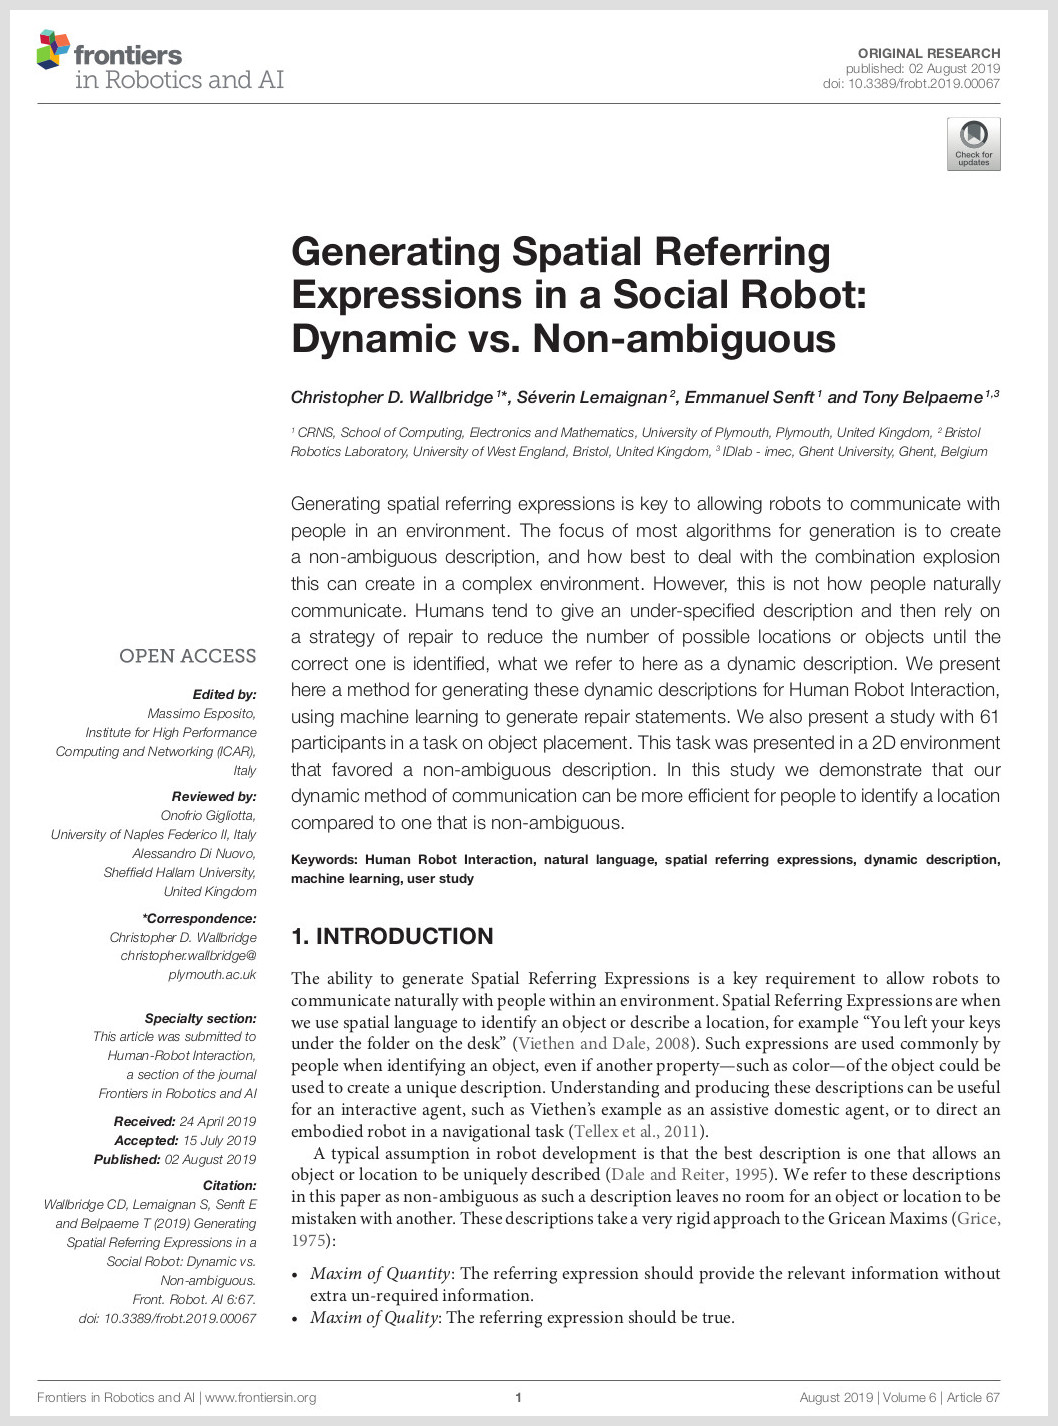
\includegraphics[height=2.2cm]{thumbs/2019-frontiers-chris.jpg} &

    Wallbridge, C., \ul{Lemaignan, S.}, Senft, E., Belpaeme, T.  
    \newline\href{https://doi.org/10.3389/frobt.2019.00067}{\textbf{Generating
    Spatial Referring Expressions in a Social Robot: Dynamic vs Non-Ambiguous}}
    \newline \textit{Frontiers in AI and Robotics} 2019
    & \small Challenges the common understanding that robots should be
    unambiguous: we show that ambiguity is often desirable for fluid and natural
    human-robot interactions.\textbf{\newline[main study supervisor]}  \\

    \vspace{-.20cm}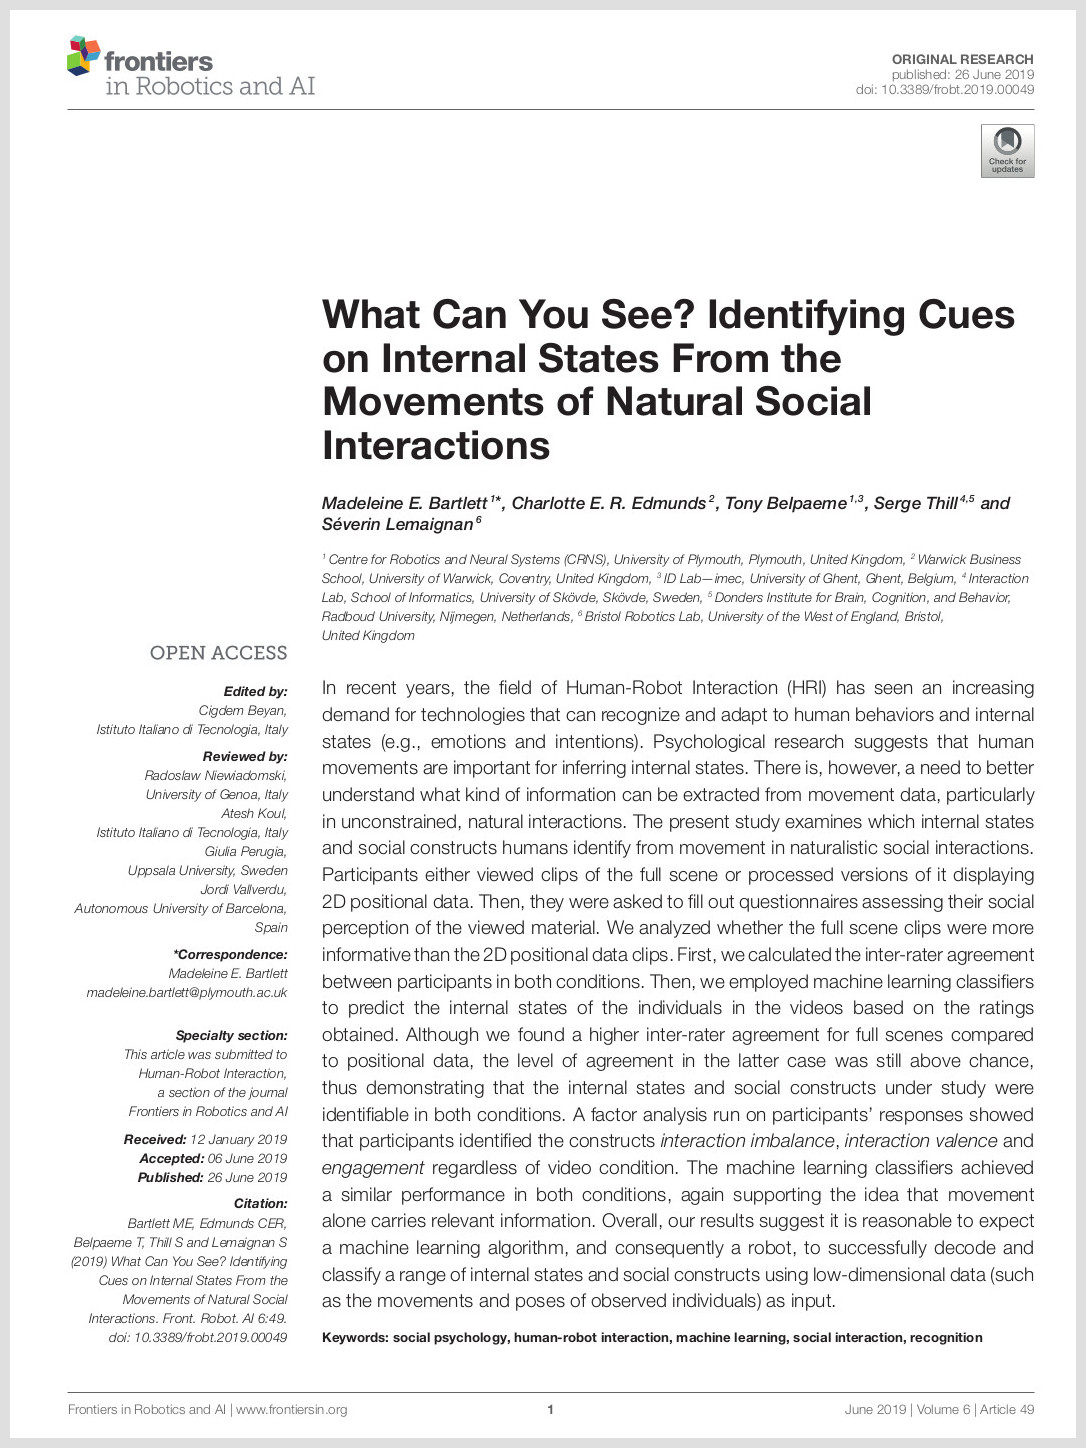
\includegraphics[height=2.2cm]{thumbs/2019-frontiers-maddy.jpg} &

    Bartlett, M., Edmunds, C. E. R., Belpaeme, T., Thill, S., \ul{Lemaignan, S.} 
    \href{https://doi.org/10.3389/frobt.2019.00049}{\textbf{What Can You See? Identifying Cues on Internal States from the
    Kinematics of Natural Social Interactions}} 
    \newline \textit{Frontiers in AI and Robotics} 2019
    & \small Investigates how partially hidden 'internal states' (like emotions,
    cooperativeness, etc) can be decoded from simple visible cues, like
    skeletons. Also demonstrates that social situations can be described along 3
    simple dimensions.\textbf{\newline[main study supervisor]}\\


    \vspace{-.20cm}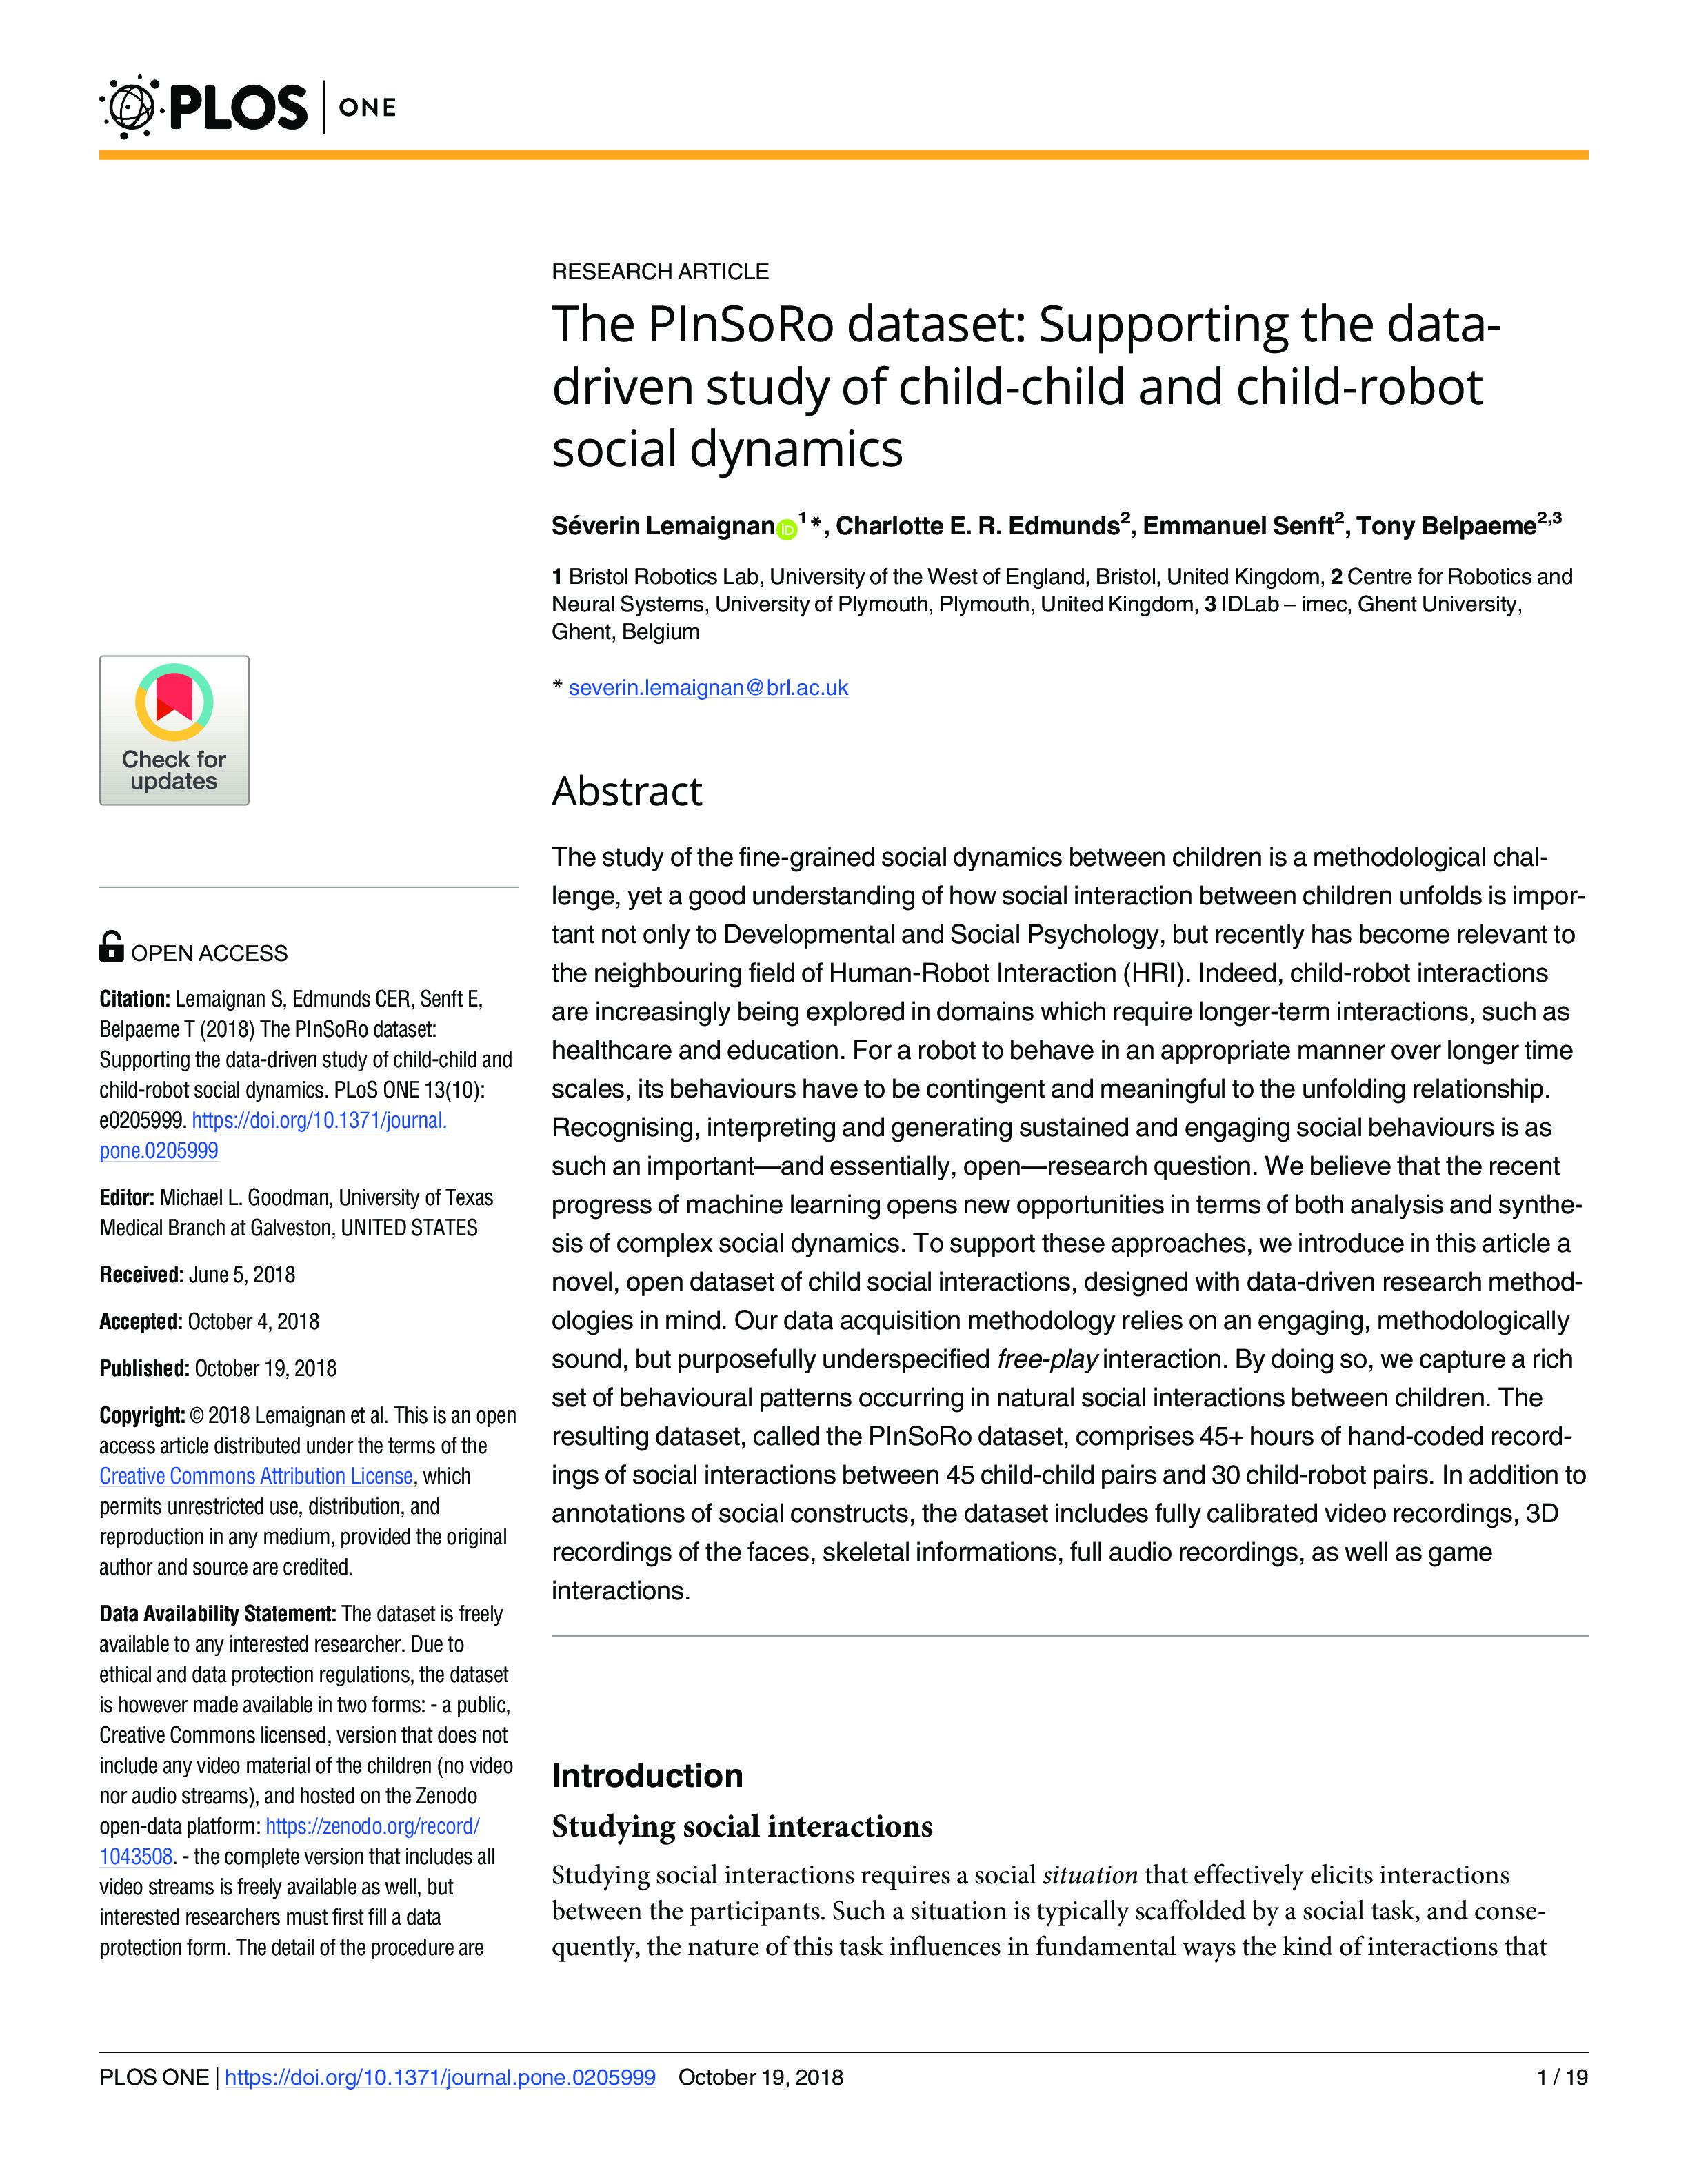
\includegraphics[height=2.2cm]{thumbs/2018-plosone.jpg} &

    \ul{Lemaignan, S.}, Edmunds E. R., C., Senft, E., Belpaeme, T.
    \newline\href{https://doi.org/10.1371/journal.pone.0205999}{\textbf{The
    PInSoRo dataset: Supporting the data-driven study of child-robot social
    dynamics}}
    \newline \textit{PLOS ONE} 2018
    & \small A first-in-kind, large scale dataset of child-child and child-robot social interactions. Design
    with machine learning in mind, this dataset effectively opens up the field
    of data-driven social psychology, with direct applications in AI and social
    robotics.\textbf{[principal investigator]}\\

    \vspace{-.20cm}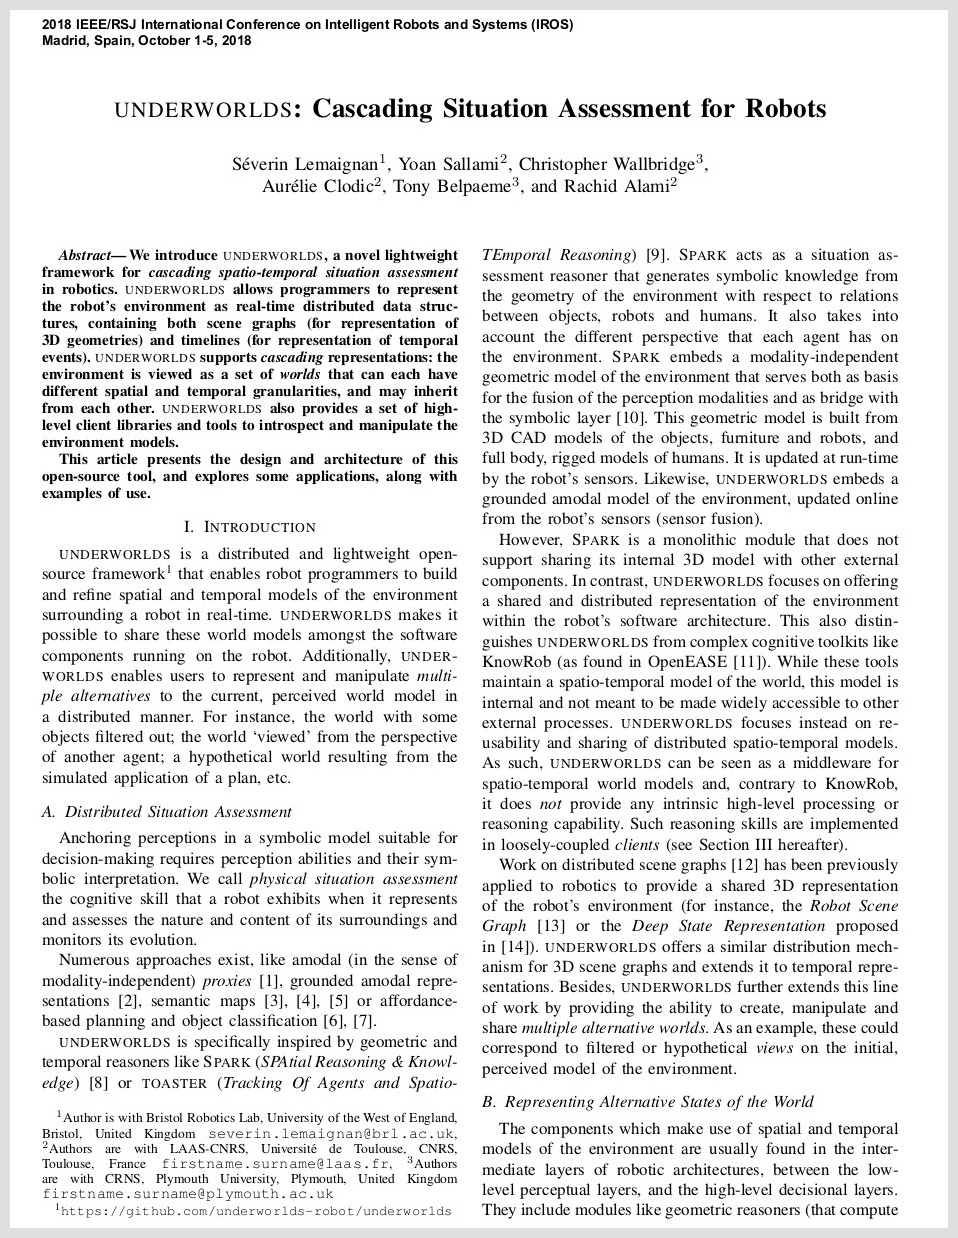
\includegraphics[height=2.2cm]{thumbs/2018-underworlds.jpg} &

    \ul{Lemaignan, S.}, Sallami, Y., Wallbridge, C., Clodic, A., Alami,
    R. 
   \newline\href{https://doi.org/10.1109/IROS.2018.8594094}{\textbf{\sc
    underworlds: Cascading Situation Assessment for Robots}}
    \newline\textit{IEEE IROS} 2018

    & \small A novel representation technique to efficiently
    represent multiple parallel states of the world, including imaginary ones.
    This ability is critical to represent spatio-temporal predictions, and to
    create models of other agents' representations.
    \textbf{[principal investigator]}\\



    \vspace{-.20cm}
\includegraphics[height=2.2cm]{thumbs/2017-sparc.jpg} &

    Senft, E., Baxter, P., Kennedy, J., \ul{Lemaignan, S.}, Belpaeme, T.
    \newline\href{https://doi.org/10.1016/j.patrec.2017.03.015}{\textbf{Supervised
    Autonomy for Online Learning in Human-Robot Interaction}}
    \newline \textit{Pattern Recognition Letters} 2017
    & \small The mathematical and technical bases of the SPARC
    paradigm for human-in-the-loop machine learning, showing that
    high-dimensional problems can be learnt effectively and rapidely thanks to
    an innovative input feature selection mechanism.
    \textbf{\newline[student supervisor; 22 citations]}\\


    \vspace{-.20cm}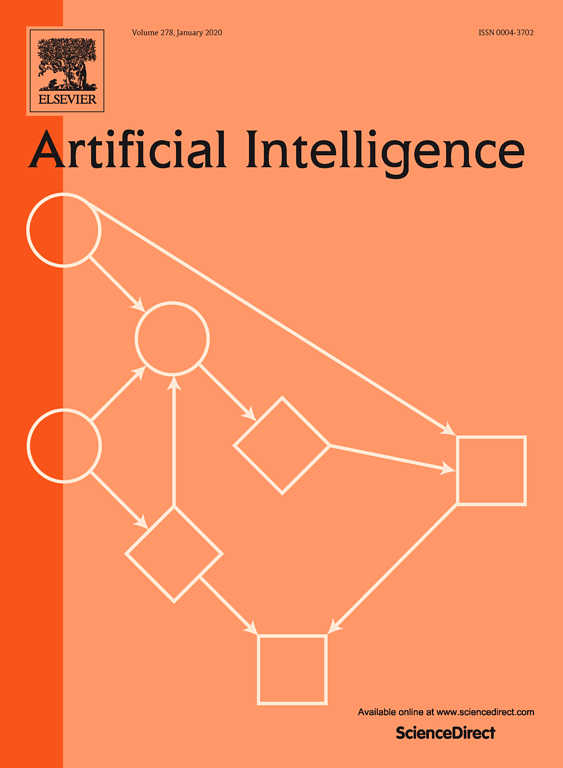
\includegraphics[height=2.2cm]{thumbs/2017-ai-cover.jpg} &

    \ul{Lemaignan, S.}, Warnier, M., Sisbot, E.A., Clodic, A., Alami, R.
    \newline
    \href{https://doi.org/10.1016/j.artint.2016.07.002}{\textbf{Artificial
    Cognition for Social Human-Robot Interaction: An Implementation}}
    \newline \textit{Artificial Intelligence} 2017
    & \small Landmark article: one of the first complete, semantic-aware, robotic architecture for
    human-robot interaction, including symbolic knowledge representation,
    situation assessment, natural language grounding, task planning, human-aware
    motion planning and execution. \textbf{\newline[principal investigator and
    coordinator; 140 citations]}\\


    \vspace{-.20cm}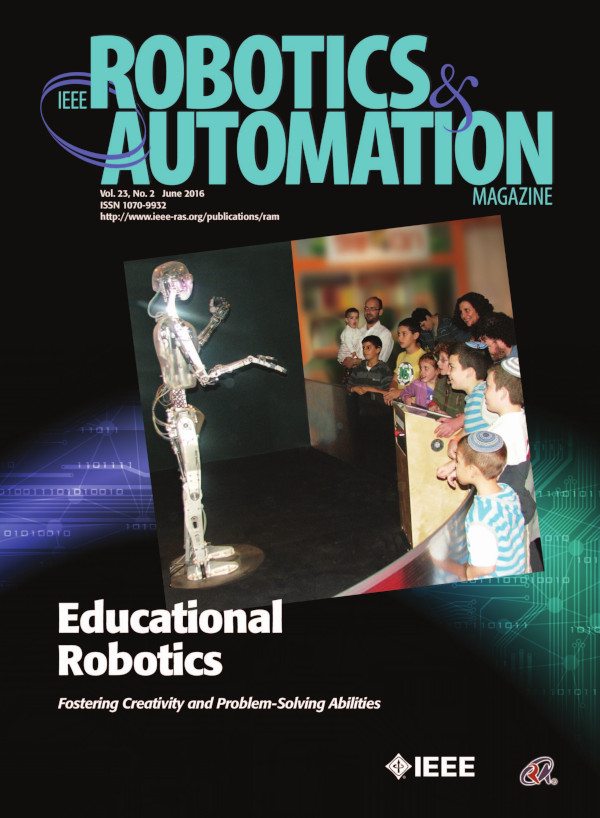
\includegraphics[height=2.2cm]{thumbs/2016-cowriter.jpg} &

    \ul{Lemaignan, S.}, Jacq, A., Hood, D., Garcia, F., Paiva, A., Dillenbourg, P.
    \newline
    \href{https://doi.org/10.1109/MRA.2016.2546700}{\textbf{Learning by
    Teaching a Robot: The Case of Handwriting}}
    \newline \textit{Robotics and Automation Magazine} 2016
    & \small Long-term studies with children and
    therapists, where we \emph{reverse} the social role of the
    robot to significantly improve the children' self-confidence. A landmark in
    social robotics for education. \textbf{\newline[principal investigator; 141
    citations} (incl. conf. article) \textbf{]}\\


    \vspace{-.20cm}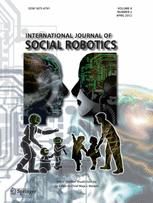
\includegraphics[height=2.2cm]{thumbs/2012-grounding.jpg} &

    \ul{Lemaignan, S.}, Ros, R., Sisbot, E. A., Alami, R., Beetz M.
    \href{https://doi.org/10.1007/s12369-011-0123-x}{\textbf{Grounding
    the Interaction: Anchoring Situated Discourse in Everyday Human-Robot
    Interaction}} 
    \newline \textit{Intl Journal of Social Robotics} 2012

    & \small In this paper, I show how symbolic knowledge representation can be
    used by robot to ground natural language interactions, also taking into
    account the unique perspective of the human interactor.
    \textbf{\newline[principal investigator; 100 citations]}\\

    \vspace{-.20cm}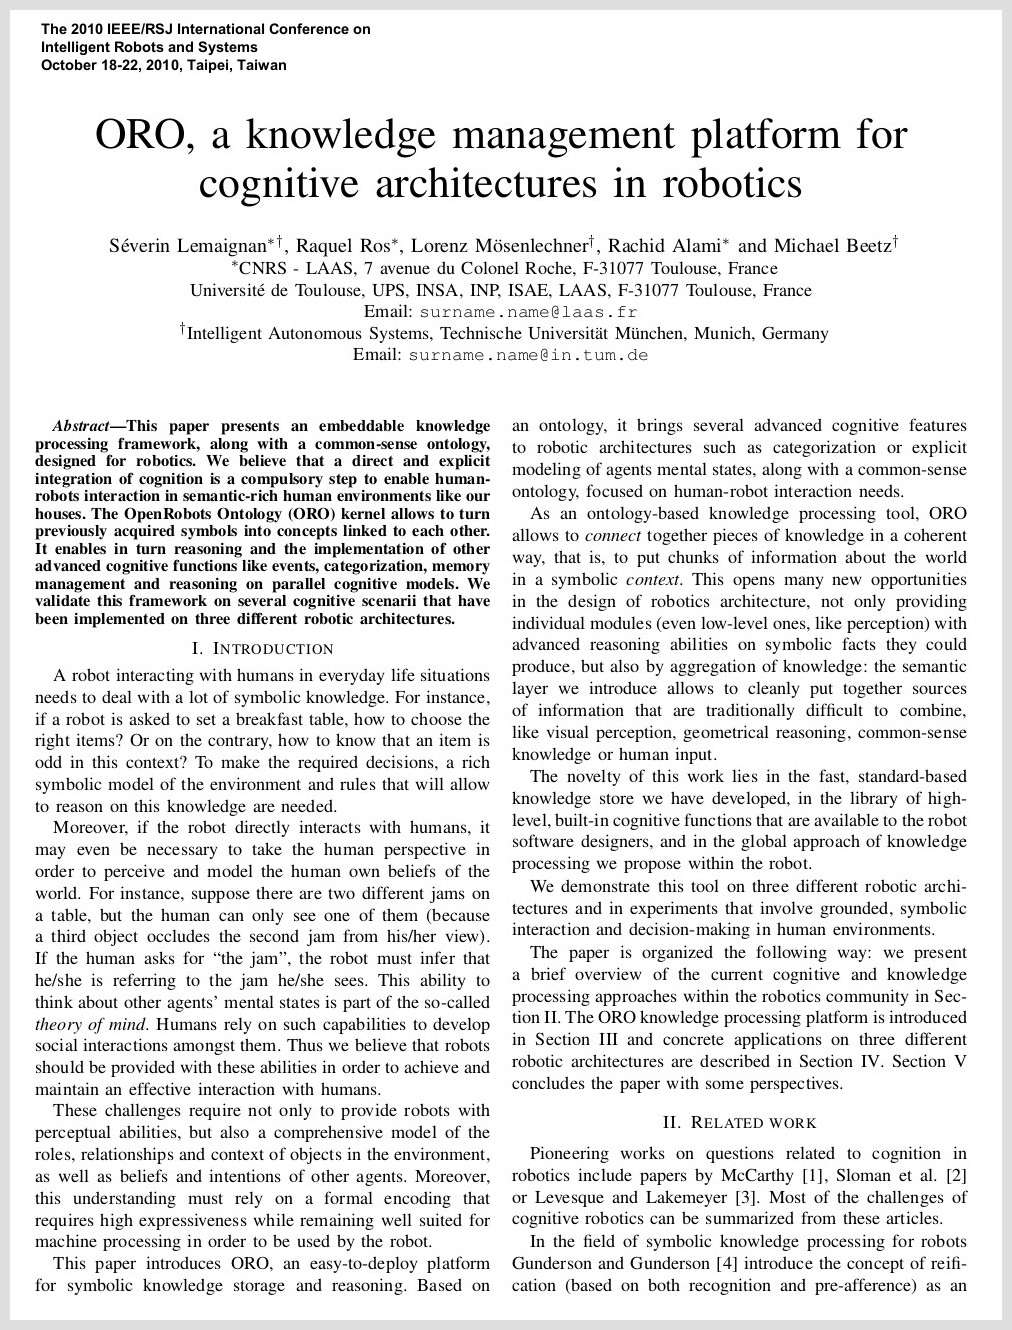
\includegraphics[height=2.2cm]{thumbs/2010-oro.jpg} &
    \ul{Lemaignan, S.}, Ros, R., Mösenlechner, L., Alami, R., Beetz, M.
    \newline\href{https://doi.org/10.1109/IROS.2010.5649547}{\textbf{ORO, a Knowledge Management Module for Cognitive Architectures in
    Robotics}}
    \newline \textit{IEEE IROS} 2010

    & \small One of the very first knowledge base designed and
    integrated in service robots. Pioneering work which played a key role in
    understanding how intelligent robot can represent their
    knowledge to facilitate communication with humans.
    \textbf{\newline[principal investigator; 155 citations]}\\

\end{tabular}
%}



%\subsection{Host institution}\label{host-institution}}
%
%The \emph{Bristol Robotics Laboratory (BRL)} is the largest co-located
%and most comprehensive advanced robotics research establishment in the
%UK. It is a joint venture between the University of the West of England
%and the University of Bristol. BRL's multidisciplinary approach aims to
%create autonomous devices capable of working independently, with each
%other, or with humans. BRL draws on robotics, electrical \& mechanical
%engineering, computer science, psychology, cognitive science and
%sociology. BRL has an international reputation as a leading research
%centre in advanced robotics research and has over 250 researchers
%working on a broad portfolio of topics: HRI, collective robotics, aerial
%robotics, neuro-inspired control, haptics, control systems, energy
%harvesting and self-sustaining systems, rehabilitation robotics, soft
%robotics and biomedical systems. BRL has many collaboration
%partnerships, both national and international, and is experienced in
%managing large multi-site projects. BRL has support from two embedded
%units specialising in business and enterprise, together with an
%incubator and successful track record of spin-outs.





%%%%%%%%%%%%%%%%%%%%%%%%%%%%%%%%%%%%%%%%%%%%%%%%%%%%%%%%%%%%%%%%%%%%%%%%%%%%%
%%%%%%%%%%%%%%%%%%%%%%%%%%%%%%%%%%%%%%%%%%%%%%%%%%%%%%%%%%%%%%%%%%%%%%%%%%%%%
%%%%%%%%%%%%%%%%%%%%%%%%%%%%%%%%%%%%%%%%%%%%%%%%%%%%%%%%%%%%%%%%%%%%%%%%%%%%%

\newpage



%%%%%%%%%%%%%%%%%%%%%%%%%%%%%%%%%%%%%%%%%%%%%%%%%%%%%%%%%%%%%%%%%%%%%%%%%%%%%
%%%%%%%%%%%%%%%%%%%%%%%%%%%%%%%%%%%%%%%%%%%%%%%%%%%%%%%%%%%%%%%%%%%%%%%%%%%
%%%%%%%%%%%%%%%%%%%%%%%%%%%%%%%%%%%%%%%%%%%%%%%%%%%%%%%%%%%%%%%%%%%%%%%%%%%
\newpage
\newrefsection
\chapter{B2.a State-of-the-art and objectives}

\TODO{SECTION B2.a IS HEAVILY WORK IN PROGRESS! many blocks of text are missing
or not at the right place}


\eu{(B2.a, B2.b, B2.c: max 15 pages (2 pages for B2.c)}
\eu{Specify the proposal objectives in the context of the state
of the art in the research field. It should be clear how and why the proposed work is important for
the field, and what impact it will have if successful, such as how it may open up new horizons or
opportunities for science, technology or scholarship. Specify any particularly challenging or
unconventional aspects of the proposal, including multi- or inter-disciplinary aspects.}

\TODO{as a reference: DECRESIM project: 4 pages on B2.a State of art and objectives; B2.b ~7 pages on WPs + 2 pages on risk assessment}


\project is also a highly technical project, who aims at significantly
pushing the state-of-art in autonomous social robotics. Indeed, in \project, we will
\textbf{implement the AI required for robots to effectively support
human social interactions}.  In that sense, this research is also
ground-breaking in regards to its technical objectives. In \project, robots will
be able to understand complex social dynamics, and generate appropriate social
responses, in a fully autonomous way.  Extending the current line of research of
the PI, we will identify, implement, and integrate the a broad range of cognitive functions into a
principled, socially-driven, and trustworthy socio-cognitive architecture for
robots. This is the second major expected scientific outcome of \project.

%%%%%%%%%%%%%%%%%%%%%%%%%%%%%%%%%%%%%%%%%%%%%%%%%%%%%%%%%%%%%%%%%%%%%%%%%%%%%%%
\subsection{The case for robot-supported human-human interactions}

This change of paradigm (rHHI) will have
far reaching impact on the place that we collectively assign to social robots in
the society; it will help to structure the public debate by providing the
framing to look at human-robot interactions in term of their net social utility.
As such, \textbf{the first outcome of \project will be researching, defining and implementing the conceptual
framework that we need to ensure trustworthy and socially responsible robots in
our societies}.


Indeed, in a time where robots are on the verge of becoming pervasive in our
daily human environment, can we ensure 'by design' that robots are to become
powerful tools to support more and better, positive interactions \emph{between
the people themselves}, and build a stronger, more cohesive society? Beyond
Human-Computer Interaction (HCI) and Human-Robot Interaction (HRI), \project is
a forward-looking, ground-breaking project that aims at establishing
\textbf{Robot-supported Human-Human Interactions (r-HHI)} as the next step
toward a Responsible AI: \textbf{the scientific investigation of how social
robots can create, shape and support strong, sustained, positive
\emph{human-human} relationships}.

As a researcher who has been working for the last 12 years in the field of
human-robot interaction (and child-robot interaction in particular), I have been
a direct witness -- by being one of the architects -- of the crossing of a
critical milestone: the emergence of \textbf{long-term social interactions}
between robots and humans. Over the last two years in particular, we observe an
explosion of the number of studies involving social robots, deployed in
real-world settings (schools, care centres) over relatively long periods of time
(up to 2 or 3 months at a time)~\cite{kunze2018artificial,leite2013social}. Even
though these robots are rarely fully autonomous, they do already show high
levels of autonomy~\cite{senft2019teaching}, with full autonomy in
sight~\cite{hawes2017strands}.

While many see these developments positively,
others express skepticism or worry that this technology might lead to a
dehumanisation of our society. Indeed, if artificial agents are to engage into
social interactions with us, and enter what many view as a form of a 'private
domain', reserved to humans, pressing ethical questions need to be answered:

\begin{itemize}
    \item how to ensure that social robots are not used to simply replace the human
        workforce to cut costs?
    \item can we provide guarantees that the use of social robots will always be
        ethically motivated?
    \item further on, can we implement some ethical safeguarding built-in
        the system (like an ethical \emph{black-box}~\cite{winfield2017case})?
    \item what about privacy? how to trust robots in our home or school or
        hospital not to eavesdrop on our private lives, and, in the worst
        case, not be used \emph{against} us?
\end{itemize}

These questions are not only legitimate, but also pressing. The recent rise of
personal assistants like Amazon Alexa or Google Home, with the major privacy
concerns that accompanies their deployments in people home, shows that letting
the industry set the agenda on these questions is not entirely wise -- and
robots can potentially be much more intrusive than non-mobile smart speakers.
The EU is positioning itself at the forefront of those questions. The recent
release of operational \emph{Ethics Guidelines for Trustworthy AI} by the EU
High-level Expert Group on Artificial Intelligence~\cite{eu2019ethics} is a
strong sign of this commitment.  However, personal \& social robots raise a new
class of questions regarding what ethical and trustworthy systems might look
like, and while the principles of responsible design are somewhat
established~\cite{stahl2016ethics, bsi2016robots}, the reality of
robot-influenced social interactions is not understood yet, if only because the
technology required to experience such interactions is only slowly maturing. 

Social robots have indeed two properties that stand out, and distinguish them from
these smart speakers, while making them significantly harder to conceptually frame.
First, they are fully embodied, and they physically interact with their
environment, from moving around, to picking up objects, to looking at you;
second, willingly or not, they are ascribed \emph{agency} by people. This second
difference has far-reaching consequences, from affective bonding to over-trust,
to over-disclosure of personal, possibly sensitive,
informations~\cite{martelaro2016tell,shiomi2017robot}.


Due to the complex interplay between the socio-psychological determinants of the
interactions, the technical implementation, and the multiple ethical mechanisms
that have to be built-in the system, it is difficult to build one coherent and
consistent perspective on the whole question. Indeed, the conceptual,
intellectual framework emcompassing both the internal cognitive mechanisms
required by socially intelligent robots, as well as their role and impact in the
society, only exists in fragmented, disconnected pieces~\cite{citeneeded}.


The lack of such a proper conceptual framing is a critical issue: for robots to
have a positive impact on the society, with strict ethical and privacy-related
safeguarding, it is urgent that the wider academic and intellectual communities,
beyond technologists, embrace this question and build up the debate on the
acceptability of robots in our society. And \textbf{this also calls for a major
re-thinking of the traditional paradigm of Human-Robot Interaction}.
Tradionally, individual cognitive functions (like natural language processing,
emotion recognition, proxemics-aware navigation) are implemented in robots, with
the ill-supported assumption that 'the more available functions, the more
socially-capable the robot'. This assumption is questionable, and, at any rate,
does not address the 'why': why does the robot decides to do what it does? What
drives the behaviour of the robot? The case for \emph{teleological} (ie
goal-driven) robotic architectures has been made in the
past~\cite{wrede2012towards}, but only effectively realised for relatively
simple cognitive systems (like curiosity-driven robot
animals~\cite{oudeyer2005playground} or motor babbling in infant-like
robots~\cite{forestier2017unified}). However, socially-driven robots,
participating in complex interactions with humans, have been barely
investigated. We need to create a new social purpose, a new social teleology to
drive the development of social robots.  Indeed, \textbf{being socially-driven
to do 'good' is essential in ensuring trustworthy, socially responsible robots}.
Nutrured by decades of research in understanding human social cognition and its
social motivations, one of the key purpose of \project is to \textbf{research
and build a principled and socially-driven cognitive architecture} for
tomorrow's social robots. This socially-driven, teleological architecture,
intrinsically designed to \textbf{support stronger, positive human-human
interactions} is what underpins the concept of \emph{robot-supported human-human
interactions}.

%%%%%%%%%%%%%%%%%%%%%%%%%%%%%%%%%%%%%%%%%%%%%%%%%%%%%%%%%%%%%%%%%%%%%%%%%%%%%%%

While the original poster picture of a
'multi-function-household-robot-that-does-the-dishes' has yet to materialise,
social robots are certainly in the process of establishing themselves as
important agents in a variety of other situations, for their intrinsic
\emph{social} features: source of comfort, tutors, entertainers. The robot as a
\emph{social agent} is a reality, within laboratories at least.

\subsection{The long-term vision: robot-supported human-human interactions}


\begin{figure}
\centering
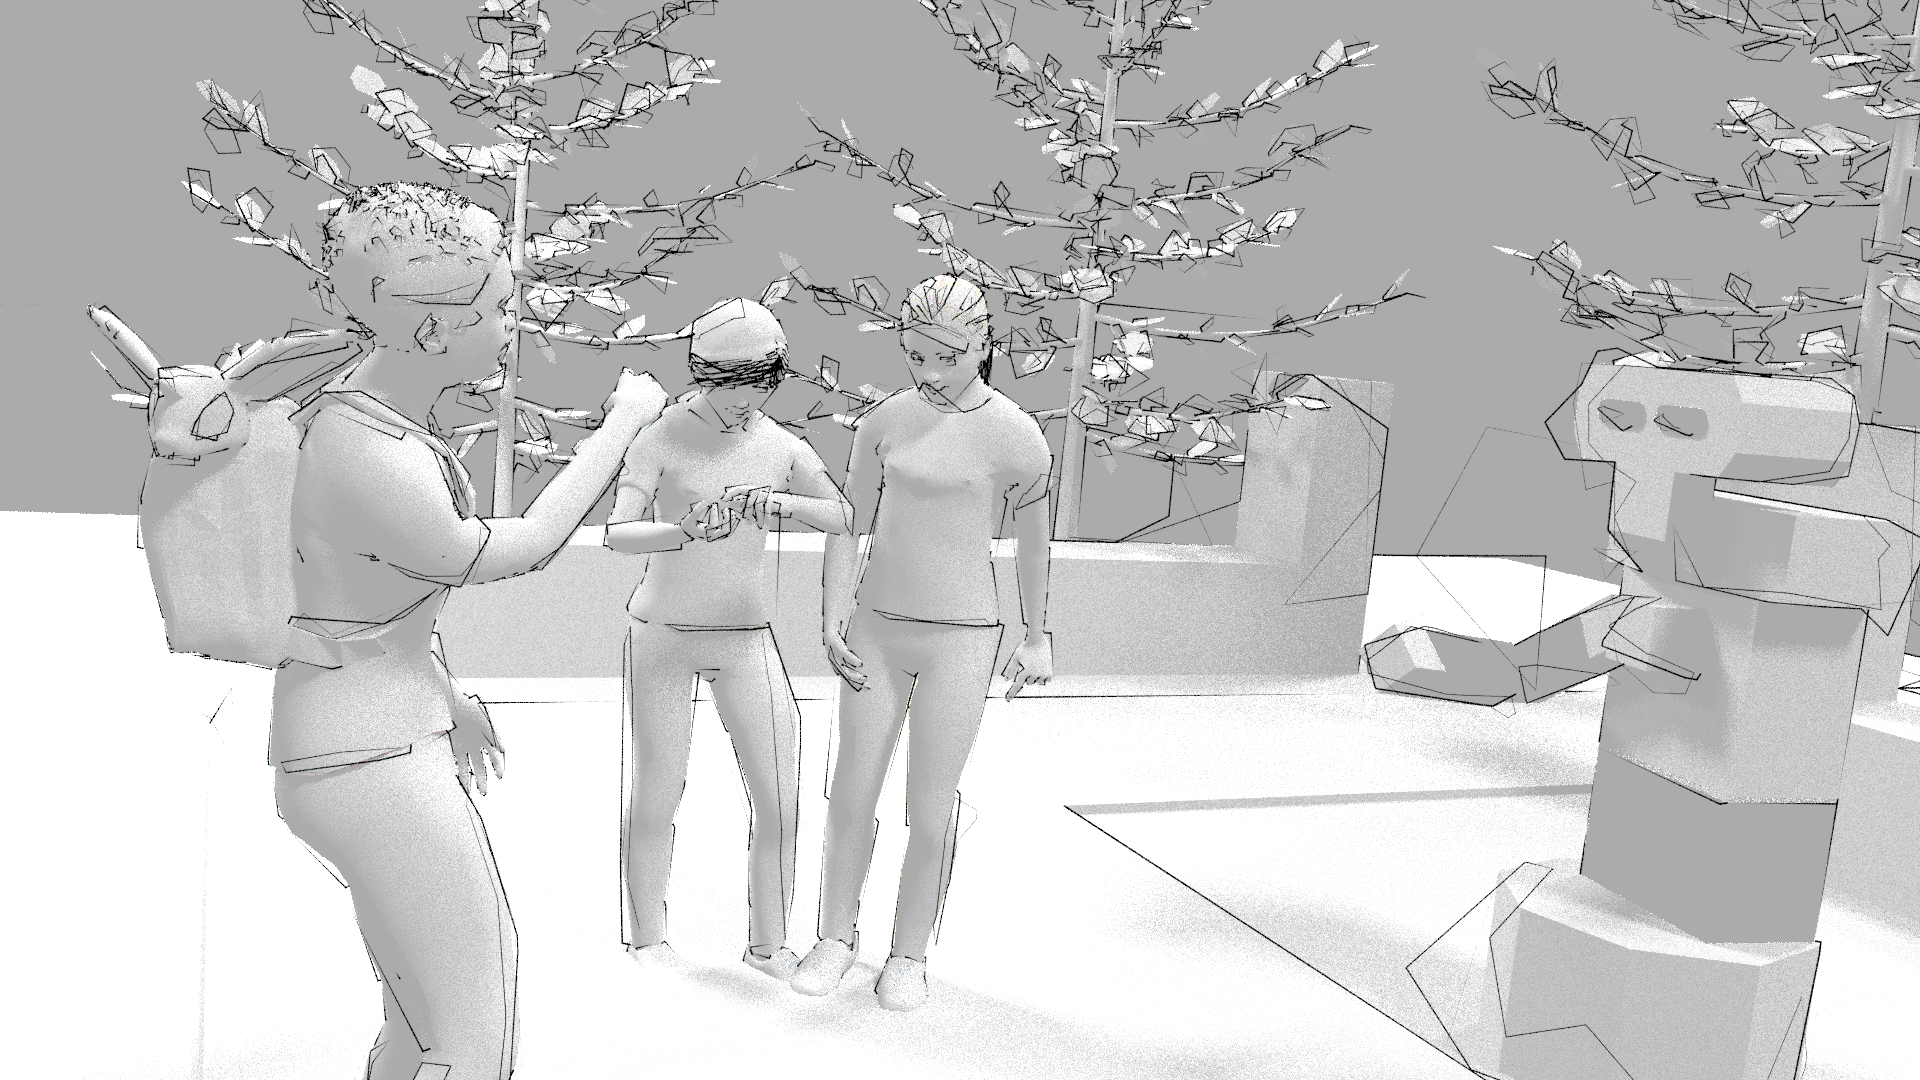
\includegraphics[width=0.9\linewidth]{figs/rHHI-1}
\caption{A child, just arriving in a new school, tries to integrate with other
    children -- in such a situation, should the robot decide to help to break the ice? What
    are the socio-cognitive peceptual and behavioural capabilities required to
    make that decision?}
\label{fig:rHHI}
\end{figure}


\project is a project that aims at helping to build strong human
relationships with the help of technology.

The core idea of the project is to build small companion robots whose
aim is to facilitate human-human interactions. We want to develop these
robots with a particular application in mind: supporting the social and
cultural integration of vulnerable children in a foreign country, and in
particular, migrant children who might lack the otherwise needed support
(shared culture; already well integrated relatives) for a successful
integration.

\subsubsection{Key scientific research questions}

\begin{enumerate}
\item research the role of social influence to scaffold positive human-human
    interactions (including its ethical ramifications) in the context of migrant
    integration;
\item explore how a small robot companion can be endowed with social
    competencies to positively influence human interactions; design and
    implement the corresponding artificial social behaviours;
\item design and build a small rugged and autonomous companion robot that
    realise this goal for child-child interactions; test the technology in
    school with actual migrant children.
\end{enumerate}


\subsection{Three pillars}

The \project project will, for the first time, take a broad, holistic approach
to these questions, and as such, is build around three pilars:

\begin{enumerate}
    \item AI architecture for decision making
    \item socio-psychological design of the interaction, from 1-to-1
        interaction, to group interaction, to interaction with the eco-system
    \item built-in privacy and ethics
\end{enumerate}

The difficulty comes from the fact that these pilars do not represent independent
research questions: they are deeply woven together, in intricate ways.

Taken independently, these three pilars are already intrinsically complex.

The first pilar, AI Architecture for Decision Making, for instance:
state-of-the-art decision making processes for social robots are build from
multiple algorithmic layers: classical machine learning (like classifiers, or
SLAM) for low-level sensori-motor processing; probabilistic data processing (for
e.g. localisation or point cloud processing); deep neural networks for object
recognition, scene understanding, speech and dialogue processing; classical
symbolic reasoning (for instance, for task planning); high-level knowledge
representation and reasoning (semantic webs); hybrid spatial/symbolic reasoning
for motion planning; etc.

Importantly, these layers are not typically combined in a simple, linear
fashion: modern control architectures are distributed, loosely coupled, and
design so that information flows in multiple directions, at different levels of
abstraction, in order to create complex feedback loops, and achieve systems that are
both goal-directed \emph{and} reactive (event-driven).


The real complexity of such AI architectures is however striking when one tries
to answer \emph{how} such an architecture can enable the realisation of the
desired socio-cognitive functions, i.e. our second pilar. Social behaviours and
social situations are highly dynamic, loosely structured, underspecified (no
pre-made rulebook exists), uncertain.

Our best answer is for the robot to learn to become social: a human expert teaches
the robot how to socially behave, in-situ, with the robot embedded in the
interaction. I have conducted two recent and high-profile experiments in this
direction


%%%%%%%%%%%%%%%%%%%%%%%%%%%%%%%%%%%%%%%%%%%%%%%%%%%%%%%%%%%%%%%%%%%%%%%%%%%%%%%
%%%%%%%%%%%%%%%%%%%%%%%%%%%%%%%%%%%%%%%%%%%%%%%%%%%%%%%%%%%%%%%%%%%%%%%%%%%%%%%
%%%%%%%%%%%%%%%%%%%%%%%%%%%%%%%%%%%%%%%%%%%%%%%%%%%%%%%%%%%%%%%%%%%%%%%%%%%%%%%
\section{[Blocks of text for reuse]}


im robots can have a lasting, positive
impact on the society, by fostering social interactions amongst humans
themselves. It defines the new concept of \textbf{robot-supported human-human
interactions} as a general framework to study and implement socially-aware
intelligent robots, able to understand social interaction, and, when
appropriate, act to create and support positive interactions between people.


Grounded in both the psycho-social literature of human cognition, and the latest
technological advances in human-robot interaction, the project delivers
major conceptual, technical and experimental contributions to the field of AI, 
with a particular focus on ethics \& safeguarding mechanisms, in order to build 'by 
design' a trustworthy AI system.

\project delivers this programme by building on a range of multidisciplinary
methods, including sociological investigation, novel interactive machine
learning techniques, and a pervasive approach to co-design that puts the
end-user needs at the centre of the design process. It paves the way for a
better understanding of the societal challenges raised by the rapid development
of AI and robotics, and, critically, opens a \textbf{unique window into what
positive role social robots could play in our future societies}.




\project aims at building unique European capacity to assert leadership in this
domain, and, beyond the specific deliverables of this 5-years project,
establishing the PI as a world-leader in goal-driven, socially-responsible
robotics.



While ambitious, the project's feasibility is also ensured through a strong
combination of cross-disciplinary expertise and support from the host's unique
research infrastructure. Scaffolded by a participatory and iterative research
methodology, and the PI experience in managing teams and complex projects
through his recognised leadership, \project is set to deliver.

To mirror the cross-disciplinary team, the research methodology developped for
\project will rely heavily on \emph{mutual shaping}, through co-design and
participatory design, and multi-disciplinary development sprints.

Software-wise, PI Lemaignan is a leading developer of software for intelligent
robots, with numerous contributions to the major software platforms used in
robotic (including major contributions to ROS, OpenCV, authoring of widely-used
pieces of software like the ROS-naoqi bridge used by hundred of researchers
using the Nao and Pepper robots or the MORSE robotic simulator). He has been
teaching various modules related to software development for robotics, and the
breadth and depth of his knowledge of robotic software development is well
established. He will be leading the software development, and, as part of the
fellowship, he will also seek for additional expert knowledge on (1) interaction
design and (2) low-level micro-programming to complete the set of required
programming needs.



%%%%%%%%%%%%%%%%%%%%%%%%%%%%%%%%%%%%%%%%%%%%%%%%%%%%%%%%%%%%%%%%%%%%%%%%%%%%%%%
%%%%%%%%%%%%%%%%%%%%%%%%%%%%%%%%%%%%%%%%%%%%%%%%%%%%%%%%%%%%%%%%%%%%%%%%%%%%%%%
%%%%%%%%%%%%%%%%%%%%%%%%%%%%%%%%%%%%%%%%%%%%%%%%%%%%%%%%%%%%%%%%%%%%%%%%%%%%%%%



\section{Social robots in the society}

\subsection{Psycho-social underpinnings}

Developing a conceptual framework for \emph{robot-supported human-human
interactions} implies a deep understanding of the psycho-social mechanisms at
work in human-human interactions, and in human-robot interactions.

Anthropomorphism is a psychological mechanism by which a human
ascribe human traits to non-human artefacts (here, robots): while the
robot appearance and behaviour can elicit or reinforce these ascription,
it fundamentally originate in the human her/himself~\cite{fink}.


\paragraph{A support for shared understanding}

\emph{Computer Supported Collaborative Learning} (CSCL) researches the cognitive
mechanisms and practical techniques underpinning efficient learning in social
situations. From its very beginning, CSCL research has been following
Roschelle and Teasley's suggestion~\cite{roschelle1995construction} that
collaborative learning has something to do with the process of constructing and
maintaining a \emph{shared understanding} of the task at hand. Building a shared/mutual
understanding refers to the upper class of collaborative learning situations,
those in which students should build upon each other's understanding to refine
their own understanding.  What is expected to produce learning is not the mere
fact that two students build the same understanding but the cognitive effort
they have to engage to build this shared
understanding~\cite{schwartz1995emergence}.

The construction of a shared understanding has been investigated for several
years in psycholinguistics, under the  notion of \emph{grounding}\footnote{Note
that the meaning of \emph{grounding} -- ensuring a shared understanding of a
situation during an interaction -- that we employ in this article must be
distinguished from its meaning in the context of \emph{symbol grounding} as
defined by Harnad~\cite{harnad1990symbol}.}~(Clark,
in~\cite{clark1986referring}).  However, the relevance of grounding mechanisms
for explaining learning outcomes has been questioned in learning sciences. The
monitoring and repair of misunderstanding explains for instance referential
failures in short dialogue episodes but does hardly predict \emph{conceptual
change} (ie the acquisition, acceptation and integration of a new belief into
one's mental model) over longer
sessions~\cite{dillenbourg2006sharing}. The cumulative effect of grounding
episodes can probably be better understood from a socio-cultural perspective:

\begin{quote}
Collaborative learning is associated with the increased
cognitive-interactional effort involved in the transition from \emph{learning to
understand each other} to \emph{learning to understand the meanings of the semiotic
tools that constitute the mediators of interpersonal
interaction}~\cite{baker1999role}
\end{quote}

Along this line, several scholars suggest that CSCL research should go deeper in
the understanding of how partners engage into shared meaning
making~\cite{stahl2007meaning} or \emph{intersubjective} meaning
making~\cite{suthers2006technology}.

Paradoxically, while Clark's theory is somewhat too linguistic from a conceptual
change viewpoint, it is criticized at the same time as being too cognitivist by
some psycholinguists, ie as overestimating the amount of shared knowledge and
mutual representations actually necessary to conduct a dialogue. The fundamental
issue, as old as philosophy, is the degree of coupling between the different
levels of dialogue, mostly between the lexical/syntactical level and the deeper
semantic levels. In~\cite{pickering2006alignment}, Pickering and Garrod argue
that the mutual understanding starts mostly with a \emph{superficial alignment}
at the level of the linguistic representations, due to priming mechanisms, and
that this local alignment may -- in some cases -- lead to a \emph{global
alignment} of the semantic level (\emph{deep grounding}).  For these authors,
the convergence in dialogue, and even the repair of some misunderstandings, is
explained by this mimetic behavior more than by a monitoring of each other's
knowledge: \emph{``...interlocutors do not need to monitor and develop full
common ground as a regular, constant part of routine conversation, as it
would be unnecessary and far too costly. Establishment of full common ground
is, we argue, a specialized and non-automatic process that is used primarily
in times of difficulty (when radical misalignment becomes
apparent).''}~\cite{pickering2006alignment} This view is actually not
incompatible with Clark's \emph{grounding
criterion}~\cite{clark1989contributing}: the degree of shared understanding that
peers need to reach depends upon the task they perform. For instance, a dialogue
between two surgeons might rely on superficial alignment if they talk about
their friends but has to guarantee accurate common grounds when talking about
which intervention will be conducted in which way on which patient.

Deep grounding or shared meaning making requires some cognitive load. For Clark,
what is important is not the individual effort made by the receiver of a
communicative act, but the overall \emph{least collaborative
effort}~\cite{clark1986referring}.  The cost of producing a perfect utterance
may be higher than the cost of repairing the problems that may arise through
misunderstandings. For instance, subjects are less careful about adapting their
utterances to their partner when they know they can provide feedback on his/her
understanding~\cite{schober1993spatial}. Dillenbourg et al. introduced the
notion of \emph{optimal collaborative effort}~\cite{dillenbourg1995evolution} to
stress that misunderstanding should not be viewed as something to be avoided (if
this was possible), but as an opportunity to engage into verbalization,
explanation, negotiation, and so forth.



\paragraph{Developmental pathopsychology}

The false belief experiment that we have mentioned above, was proposed by
Baron-Cohen in the frame of his research on autistic spectrum disorders (he
shows that autistic children seem to actually lack a theory of mind and suggests
this as the primary cause of their social impairments), and Frith and Happé
further note in ~\cite{frith1994autism} that this specific deficit of autism has
led to a large amount of research which proved, in turn, highly beneficial to
the study of the development of theory of mind in general. They reference
in~\cite{frith1994autism} eight such tasks (Table~\ref{mentalizing-tasks}),
identified during the study of social cognition by autistic children. Each of
them is proposed in two versions: one does not require mentalizing, while the
other does require it.  One of these tasks, for example, required children to
distinguish emotions, namely happy/sad faces on one hand (\emph{situation-based}
emotion), and surprised faces on the other (\emph{belief-based}
emotion)~\cite{baron1993children}.  Another task, based on the
\emph{penny-hiding game}, contrasts the two conditions in terms of \emph{object
occlusion} vs.~\emph{information occlusion}~\cite{baron1992out} (we detail it
hereafter). These tasks prototypically illustrate social meta-cognition: one
need to represent and reflect on someone else representations (and not only
perceptions), and they are not addressed by today's research on social robots.

Experimental protocols in research on autistic spectrum disorders are often
striking by their apparent straightforwardness because of the careful choice of
interaction modalities: since autistic children frequently exhibit impairments
beyond social ones (such as motor or linguistic ones), the experiments must be
designed such that they require only basic cognitive skills beyond the social
abilities that are tested. The Sally and Anne task, for instance, requires the
observing child to be able to visually follow the marble, to remember the true
location of the marble, to understand simple questions (``Where will Sally look
for her marble?'' in Baron-Cohen's protocol~\cite{baron1985does}) and eventually
to give an answer, either verbally or with a gesture -- the two first points
being actually explicitly checked through questions: ``Where is the marble
really?'' (reality control question) and ``Where was the marble in the
beginning?'' (memory control question).

Likewise, current social robots have limited cognitive skills (no fast yet fine
motor skills, limited speech production and understanding, limited scene
segmentation and object recognition capabilities, etc.) and such tasks
that effectively test a single cognitive skill (in this case, mentalizing) in
near isolation are of high relevance for experimental social robotics.

\begin{table}[h]
    \centering
    \begin{tabular}{p{0.4\linewidth}p{0.5\linewidth}}
        \toprule
        No mentalizing required           & Mentalizing required          \\
        \midrule
        Ordering behavioural pictures     & Ordering mentalistic pictures~\cite{baron1986mechanical} \\
        Understanding see                 & Understanding know~\cite{perner1989exploration}            \\
        Protoimperative pointing          & Protodeclarative pointing~\cite{baron1989perceptual}     \\
        Sabotage                          & Deception~\cite{sodian1992deception}                     \\
        False photographs                 & False beliefs~\cite{leslie1992domain}                 \\
        Recognizing happiness and sadness & Recognizing surprise~\cite{baron1993children}          \\
        Object occlusion                  & Information occlusion~\cite{baron1992out}         \\
        Literal expression                & Metaphorical expression~\cite{happe1993communicative}       \\
        \bottomrule
    \end{tabular}
    \caption{\small Tasks requiring or not mentalizing to pass, listed by Frith and Happé in~\cite{frith1994autism}}
    \label{mentalizing-tasks}
\end{table}

Frith and Happé's list (Table~\ref{mentalizing-tasks}) is in that regard
especially interesting in that it mirrors pairs of task (ones which do not
require mentalizing with similar ones which do require mentalizing), thus
providing control tasks.  \emph{Object occlusion} vs.~\emph{Information
occlusion} is one example of a (pair of) task(s) which evidence
representation-level perspective taking through \emph{adaptive deception}:
during a simple game, the experimenter adapts its strategy
(deceptive/non-deceptive behaviour) to the representation skills of its child
opponent. The experimental setting is derived from the penny-hiding game
protocol originally proposed by Oswald and Ollendick~\cite{oswald1989role} and
replicated and extended by Baron-Cohen in~\cite{baron1992out}, who describes it
as a two-person game in which the subject is actively involved, either as a
guesser or as a hider. The hider hides the penny in one hand or the other, and
then invites a guess. The game is repeated several time before switching the
roles. Baron-Cohen proposes a specific index to rate the level of the players
based on the idea of \emph{information occlusion}: minimally, the hider must
ensure \emph{object occlusion} (the penny must not become visible to the
guesser), while good hiders, with representation-level perspective taking
skills, develop strategies (like random hand switching or deictic hints at the
wrong hand) to prevent the guesser to find the penny (\emph{information
occlusion}). One could imagine a similar protocol adapted to robotics: the robot
would play the role of the experimenter, adapting on-line its
behaviour to what it understands of the perspective taking capabilities of the
children, and would consequently require \emph{second-order},
\emph{representation-level} perspective taking from the robot.




%%%%%%%%%%%%%%%%%%%%%%%%%%%%%%%%%%%%%%%%%%%%%%%%%%%%%%%%%%%%%%%%%%%%%%%%%%%
%%%%%%%%%%%%%%%%%%%%%%%%%%%%%%%%%%%%%%%%%%%%%%%%%%%%%%%%%%%%%%%%%%%%%%%%%%%
%%%%%%%%%%%%%%%%%%%%%%%%%%%%%%%%%%%%%%%%%%%%%%%%%%%%%%%%%%%%%%%%%%%%%%%%%%%
\section{Companion robots}

One example of a small, rugged robot designed for intensive use in school
environments is Cellulo~\footcite{ozgur2017cellulo}.

\begin{figure}[!htbp]
    \begin{minipage}[b]{.3\linewidth}
        \centering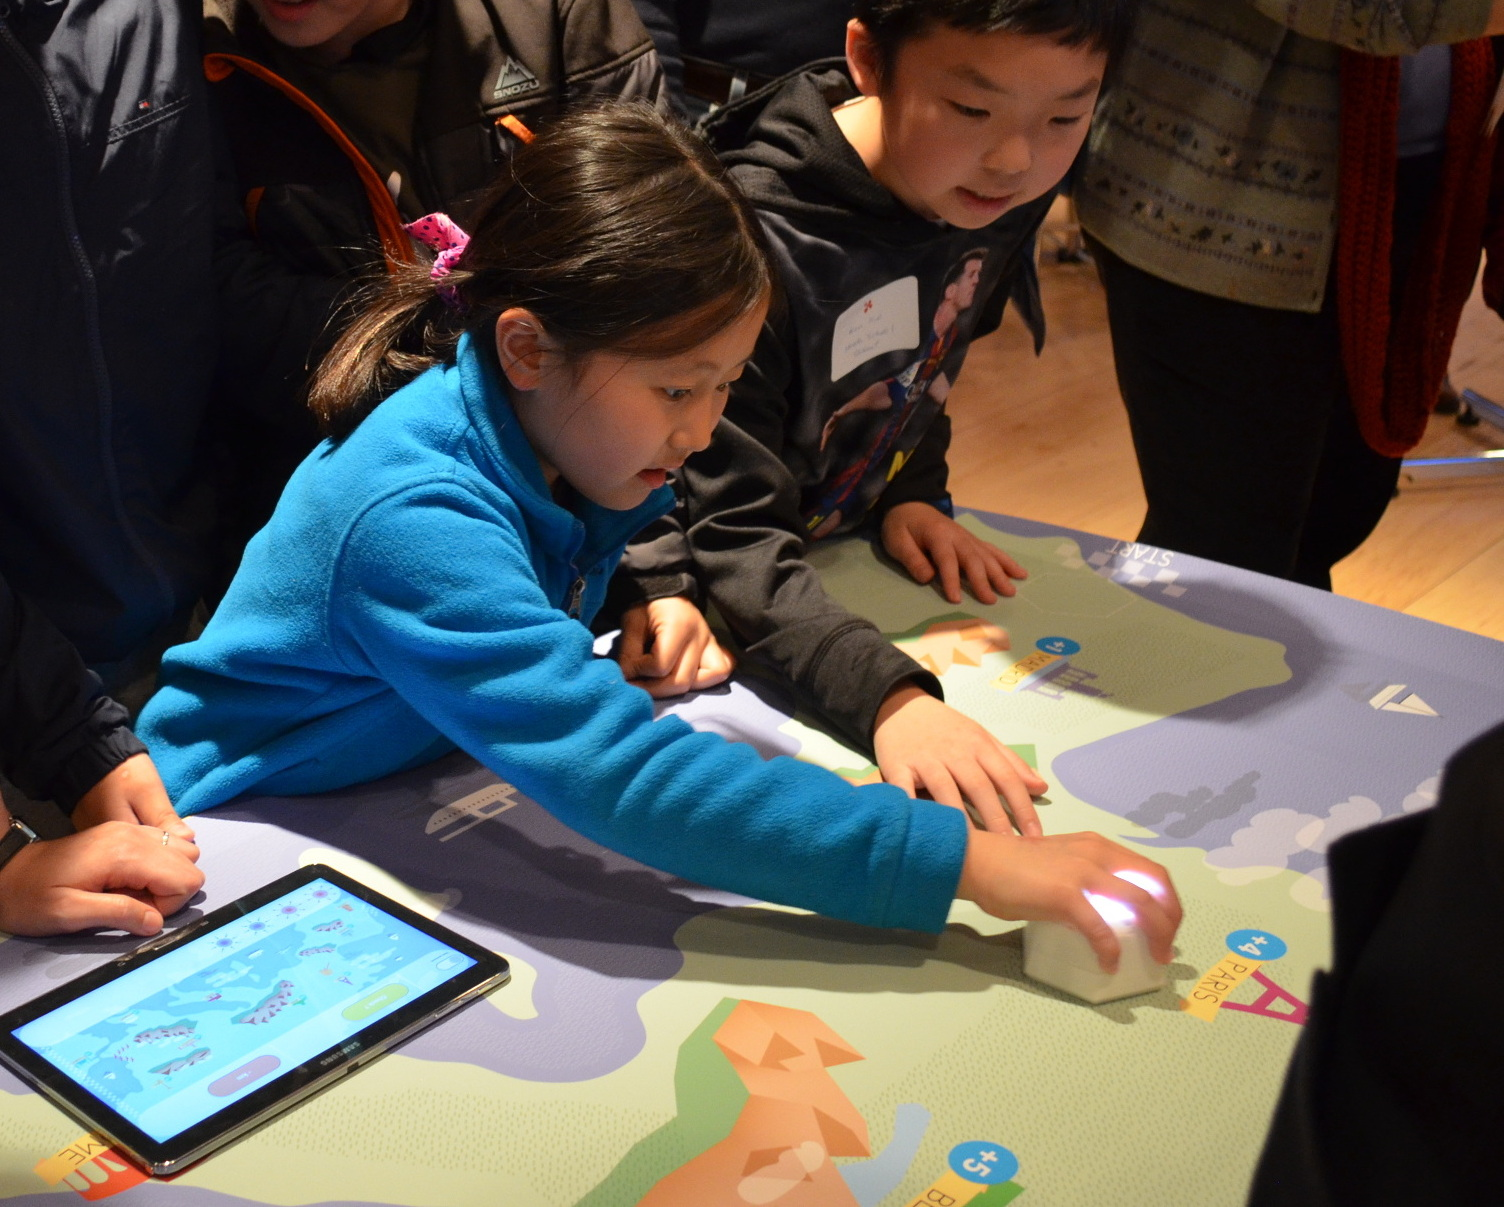
\includegraphics[height=4cm]{figs/cellulo.jpg}
        \subcaption{EPFL's Cellulo robot}\label{fig:cellulo}
    \end{minipage}%
    \hspace{0.5cm}
    \begin{minipage}[b]{.3\linewidth}
        \centering
        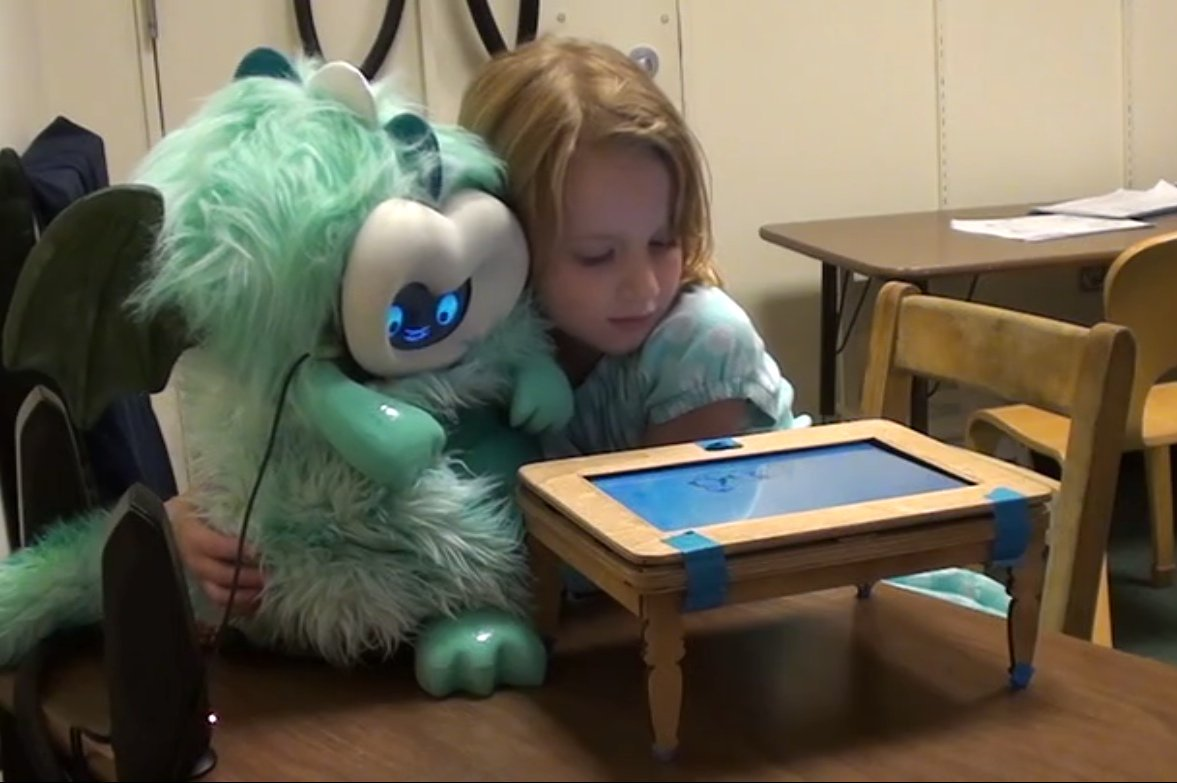
\includegraphics[height=4cm]{figs/tega.jpg}
        \subcaption{MediaLab's Tega robot}\label{fig:tega}
    \end{minipage}
    \hspace{0.5cm}
    \begin{minipage}[b]{.3\linewidth}
        \centering
        %\includegraphics[height=4cm]{figs/ono.png}
        \subcaption{OPSORO's Ono robot}\label{fig:ono}
    \end{minipage}
    \caption{Existing research-level companion robots}\label{fig:research-robots}
\end{figure}

\begin{figure}[!htbp]
    \begin{minipage}[b]{.3\linewidth}
        \centering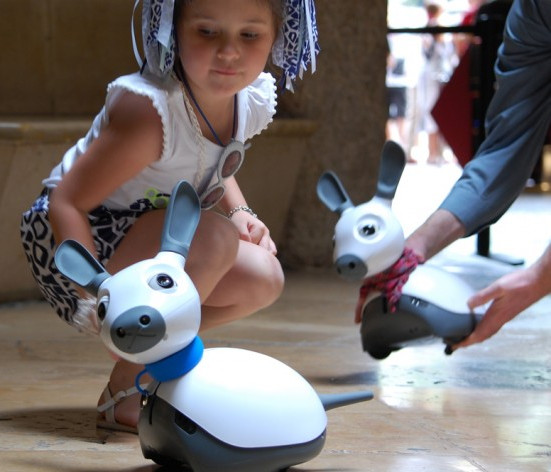
\includegraphics[height=4cm]{figs/miro.jpg}
        \subcaption{Consequential's Miro robot}\label{fig:miro}
    \end{minipage}%
    \hspace{0.1cm}
    \begin{minipage}[b]{.3\linewidth}
        \centering
        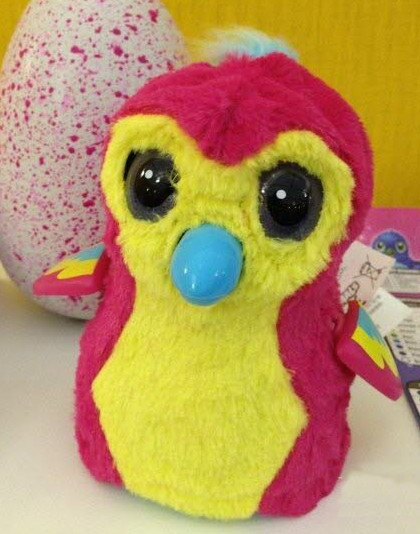
\includegraphics[height=4cm]{figs/hatchnimals.jpg}
        \subcaption{SpinMaster's Hatchimals}\label{fig:hatchimals}
    \end{minipage}%
    \hspace{0.1cm}
    \begin{minipage}[b]{.3\linewidth}
        \centering
        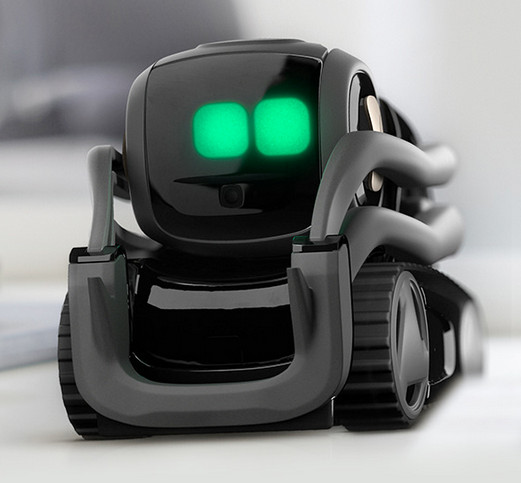
\includegraphics[height=4cm]{figs/anki-vector.jpg}
        \subcaption{Anki's Vector}\label{fig:vector}
    \end{minipage}
    \caption{Existing commercial companion robots}\label{fig:commercial-robots}
\end{figure}



\begin{figure}
    \centering
    
\includegraphics[width=0.9\linewidth]{figs/wizme+dolls}
    \caption{Early prototyping for the \project: a pet-like robot that could
    mediate child-child interactions}
    \label{}
\end{figure}



\section{Impact}\label{impact}

\subsection{Impact on society and technology: building an inclusive society}


\project will deliver new and fundamental knowledge to the fields of robotics,
computer science and psychology, in addition to improving trans-disciplinary
understanding between these disciplines. More specifically, the project will
contribute to a better understanding of the following research areas:
human-robot interaction; human-machine interaction; human error making and
handling in assembly tasks; theory of mind and its transfer to cognitive robots;
natural language processing; explainability and language generation; machine
vision and human activity detection; and action planning under uncertainty. New
interaction paradigms will be developed for handling error situations where
machines interact with non-expert humans. The integration of perception and
sensing into cognitive robot architectures will be critically reviewed and
extended. Novel, empirically informed methods to transfer findings from
human-human interaction studies to human-machine interactions will be developed.
Furthermore, the national and international psychology, robotics and computer
science research communities will benefit from the project results. We will
publish \project results in interdisciplinary and discipline-specific journals
and conferences, and organise \project-themed workshops. Please refer to Section
\ref{sec:impact} about our concrete action plan to maximise impact. 




Academically, the \project project represents a timely combination of
very recent advances in supervised machine learning for social robot
behaviour with a creative and interdisciplinary approach to the design
and automation of social robot behaviour. We therefore expect to publish
results in high-class scientific journals and conferences.

The dataset of social behaviours and social signals we will create and
distribute represents a one-in-a-kind resource for the human robot
interaction community, and the human data collection will be
transferable to research in other domains such as human-computer
interaction.

As \project will be deployed in a living lab environment, there is
significant scope for public outreach/engagement and media coverage,
which we will work with the BRL's media manager to maximise.

%%%%%%%%%%%%%%%%%%%%%%%%%%%%%%%%%%%%%%%%%%%%%%%%%%%%%%%%%%%%%%%%%%%%%%%%%%%
%%%%%%%%%%%%%%%%%%%%%%%%%%%%%%%%%%%%%%%%%%%%%%%%%%%%%%%%%%%%%%%%%%%%%%%%%%%
%%%%%%%%%%%%%%%%%%%%%%%%%%%%%%%%%%%%%%%%%%%%%%%%%%%%%%%%%%%%%%%%%%%%%%%%%%%
\chapter{B2.b Methodology}\label{research-methodology}

\eu{Describe the proposed methodology in detail including any key intermediate
goals. Explain and justify the methodology in relation to the state of the art,
and particularly novel or unconventional aspects addressing the
'high-risk/high-gain' balance. Highlight any intermediate stages where results
may require adjustments to the project planning. In case you ask that team
members are engaged by another host institution their participation has to be
fully justified by the scientific added value they bring to the project.}

%\subsection{Gantt chart}\label{gantt-chart}

\section{Workpackages overview and interrelations}\label{workpackage-interrelations}

\begin{figure}[!htbp]
    \centering
    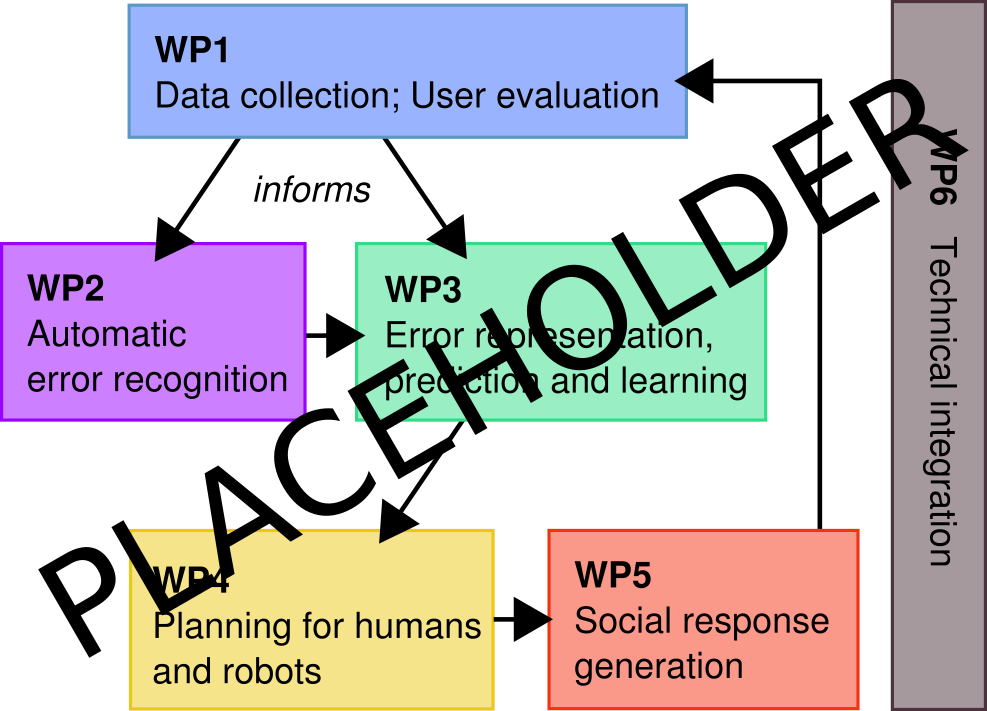
\includegraphics[width=0.8\linewidth]{figs/wp-interrelations}
    \caption{Inter-dependencies between work packages and main tasks}
    \label{}
\end{figure}

\subsection{Milestones}\label{milestones}

\begin{itemize}

\item   week-long tests with local children in local schools
\item   field deployment with one child in one school
\end{itemize}

\begin{table}[!htbp]
\caption{List of milestones}
\centering
\begin{tabular}{@{}lllll@{}}
\toprule
\textbf{Milestone number} & \textbf{Milestone name} & \textbf{Related work package(s)} & \textbf{Estimated date} & \textbf{Means of verification} \\ \midrule
                          &                         &                                  &                         &                                \\
                          &                         &                                  &                         &                                \\
                          &                         &                                  &                         &                                \\
                          &                         &                                  &                         &                                \\ \bottomrule
\end{tabular}
\end{table}


\subsection{Deliverables overview}\label{deliverables-overview}

\begin{table}[!htbp]
\caption{List of deliverables}
\begin{tabular}{@{}lllllll@{}}
\toprule
\textbf{Deliverable} & \textbf{Deliverable name} & \textbf{Work package No} & \textbf{Lead participant short name} & \textbf{Type} & \textbf{Dissemination level} & \textbf{Delivery date} \\ \midrule
D1.1                 &                           &                          &                                      &               &                              &                        \\
D1.2                 &                           &                          &                                      &               &                              &                        \\
D2.1                 &                           &                          &                                      &               &                              &                        \\
...                  &                           &                          &                                      &               &                              &                        \\ \bottomrule
\end{tabular}
\end{table}

Type:

\begin{itemize}

\item   R: Document, report (excluding the periodic and final reports)
\item   DEM: Demonstrator, pilot, prototype, plan designs
\item   DEC: Websites, patents filing, press \& media actions, videos, etc.
\item   OTHER: Software, technical diagram, etc.
\end{itemize}

Dissemination level:

\begin{itemize}

\item   PU = Public, fully open, e.g.~web
\item   CO = Confidential, restricted under conditions set out in Model Grant
  Agreement
\item   CI = Classified, information as referred to in Commission Decision
  2001/844/EC.
\end{itemize}





\begin{landscape}
%%%%%%%%%%%%%%%%%
%%
%% Task dependencies
%%
%% Task...        depends on Task...
%% T1.3           T1.1
%% T1.3           T1.2
%% T1.2           T2.2 (user interface)
%% T3.3           T2.3
%%

\definecolor{barcolor}{RGB}{153,204,254}
\definecolor{linkred}{RGB}{165,0,33}
%\renewcommand\sfdefault{phv}
%\renewcommand\mddefault{mc}
%\renewcommand\bfdefault{bc}
\setganttlinklabel{s-s}{START-TO-START}
\setganttlinklabel{f-s}{}
\setganttlinklabel{f-f}{FINISH-TO-FINISH}

%\begin{sidewaysfigure}[!ht]
\begin{figure}[!ht]

%\sffamily
\begin{ganttchart}[
        canvas/.append style={fill=none, draw=black!5, line width=.75pt},
        hgrid style/.style={draw=black!5, line width=.75pt},
        vgrid={*1{draw=black!5, line width=.75pt}},
        %vgrid={*1{black}, *{11}{black!5}}, % doesnt work for some reason
        x unit=.35cm,
        y unit chart=.65cm,
        time slot format=isodate-yearmonth,
        time slot unit=month, % pgfgantt >= 5.0
        %compress calendar, % pgfgantt < 5.0 => overleaf
        title/.style={draw=none, fill=none},
        title label font=\bfseries\footnotesize,
        %title label node/.append style={below=7pt},
        include title in canvas=false,
        bar label font=\mdseries\small\color{black!70},
        %bar label node/.append style={left=2cm},
        bar/.append style={draw=none, fill=barcolor!50},
        bar progress label font=\mdseries\footnotesize\color{black!70},
        group/.append style={fill=barcolor},
        group incomplete/.append style={fill=black},
        group left shift=0,
        group right shift=0,
        group height=.5,
        group peaks tip position=0,
        group label node/.append style={left=.6cm},
        group progress label font=\bfseries\small,
        link/.style={-latex, line width=1.5pt, linkred},
        link label font=\scriptsize\bfseries,
        link label node/.append style={below left=-2pt and 0pt,
        milestone/.append style={circle},
        milestone inline label node/.append style={left=5mm}}
    ]{2021-01}{2025-12}
    
        %\gantttitle[
        %    title label node/.append style={below left=7pt and -3pt}
        %]{Month:\quad1}{1}
        \gantttitlecalendar{year, month} \\
        %\gantttitlelist{0,5,...,60}{1} \\
        %% WP1
        \ganttgroup[]{WP1 \wpOneShort}{2021-01}{2023-12} \\
            \ganttbar[name=WP11]{\textbf{1.1} Conceptual framing \& ethics}{2021-01}{2023-12} \\
            \ganttbar[name=WP12prep,inline,bar/.append style={fill=gray!20}]{preparation}{2021-07}{2021-12}
            \ganttbar[name=WP12exp,inline]{WeTheCurious experiment}{2022-01}{2022-12}
            \ganttbar[name=WP12]{\textbf{1.2} Principles of r-HHI}{2023-01}{2023-06} \\

        %\ganttlink[link type=f-s]{WBS1A}{WBS1B}

        %% WP2
        \definecolor{barcolor}{RGB}{153,2,254}
        \ganttgroup[]{WP2 \wpTwoShort}{2021-01}{2024-12} \\
            \ganttbar[name=WP21]{\textbf{2.1} Situation assessment}{2021-01}{2022-06} \\
            \ganttbar[name=WP22]{\textbf{2.2} Social dynamics}{2022-01}{2023-12} \\
            \ganttbar[name=WP23]{\textbf{2.3} Group dynamics}{2024-01}{2024-12} \\
            \ganttbar[name=WP24]{\textbf{2.4} Social situation assessment}{2022-07}{2024-12} \\

        %\ganttlink[link type=f-s]{WP21}{WP24}
        %\ganttlink[link type=f-s]{WP22}{WP23}

        %% WP3
        \definecolor{barcolor}{RGB}{50,220,134}
        \ganttgroup[]{WP3 \wpThreeShort}{2021-01}{2025-12} \\
            \ganttbar[name=WP31]{\textbf{3.1} Social teleology}{2023-01}{2024-12} \\
            \ganttbar[name=WP32]{\textbf{3.2} Human-in-the-loop policy learning}{2021-07}{2025-06} \\
            \ganttbar[name=WP33]{\textbf{3.3} Integrated cognitive architecture}{2021-01}{2025-06} \\

        %\ganttlink[link type=f-s]{WP12}{WP32}

        %% WP4
        \definecolor{barcolor}{RGB}{244,50,20}
        \ganttgroup[]{WP4 \wpFourShort}{2022-01}{2025-12} \\
            \ganttbar[name=WP41]{\textbf{4.1} Behaviours baselining}{2022-01}{2022-12} \\
            \ganttbar[name=WP42]{\textbf{4.2} Generative behaviours}{2023-01}{2023-12} \\
            \ganttbar[name=WP43]{\textbf{4.3} Non-verbal behaviours}{2023-07}{2025-12} \\


        %% WP5
        \definecolor{barcolor}{RGB}{234,200,20}
        \ganttgroup[]{WP5 \wpFiveShort}{2022-07}{2025-12} \\
            \ganttbar[name=WP51prep,inline,bar/.append style={fill=gray!20}]{preparation}{2022-07}{2022-12}
            \ganttbar[name=WP51]{\textbf{5.1} SEN schools experiment}{2023-01}{2023-12} 
            \ganttbar[name=WP51expl,inline,bar/.append style={fill=gray!20}]{analysis}{2024-01}{2024-06} \\
            \ganttbar[name=WP52prep,inline,bar/.append style={fill=gray!20}]{preparation}{2024-01}{2024-06}
            \ganttbar[name=WP52]{\textbf{5.2} children hospital experiment}{2024-07}{2025-06}
            \ganttbar[name=WP52expl,inline,bar/.append style={fill=gray!20}]{analysis}{2025-07}{2025-12} \\

        %\ganttlink[link type=f-s]{WP41}{WP51}


        %\ganttlink[link type=f-s]{WBS1B}{WBS1C}
        %\ganttlink[link type=f-f,link label node/.append style=left]{WBS1C}{WBS1D}

        \ganttmilestone{\bf\sc Integration sprints}{2021-06}
        \ganttmilestone[milestone/.append style={fill=orange, circle}]{}{2021-11}
        \ganttmilestone{}{2022-06}
        \ganttmilestone[milestone/.append style={fill=orange, circle}]{}{2022-11}
        \ganttmilestone{}{2023-06}
        \ganttmilestone{}{2023-12}
        \ganttmilestone[milestone/.append style={fill=orange, circle}]{}{2024-05}
        \ganttmilestone{}{2024-12}


        % separate years
        \ganttvrule[vrule/.append style={gray, dotted, thin}]{}{2021-12}
        \ganttvrule[vrule/.append style={gray, dotted, thin}]{}{2022-12}
        \ganttvrule[vrule/.append style={gray, dotted, thin}]{}{2023-12}
        \ganttvrule[vrule/.append style={gray, dotted, thin}]{}{2024-12}


        \ganttvrule{start @WeTheCurious}{2021-12}
        \ganttvrule{start @SEN school}{2022-12}
        \ganttvrule{start @Children hospital}{2024-06}

\end{ganttchart}

%\end{sidewaysfigure}
\end{figure}

\end{landscape}

\newpage

%%%%%%%%%%%%%%%%%%%%%%%%%%%%%%%%%%%%%%%%%%%%%%%%%%%%%%%%%%%%%%%%%%%%%%%%%%%
%%%%%%%%%%%%%%%%%%%%%%%%%%%%%%%%%%%%%%%%%%%%%%%%%%%%%%%%%%%%%%%%%%%%%%%%%%%
\section{WP1: \wpOne{}}



%%%%%%%%%%%%%%%%%%%%%%%%%%%%%%%%%%%%%%%%%%%%%%%%%%%%%%%%%%%%%%%%%%%%%%%%%%%
%%%%%%%%%%%%%%%%%%%%%%%%%%%%%%%%%%%%%%%%%%%%%%%%%%%%%%%%%%%%%%%%%%%%%%%%%%%
\section{WP2: \wpTwo{}}

\begin{figure}
\centering
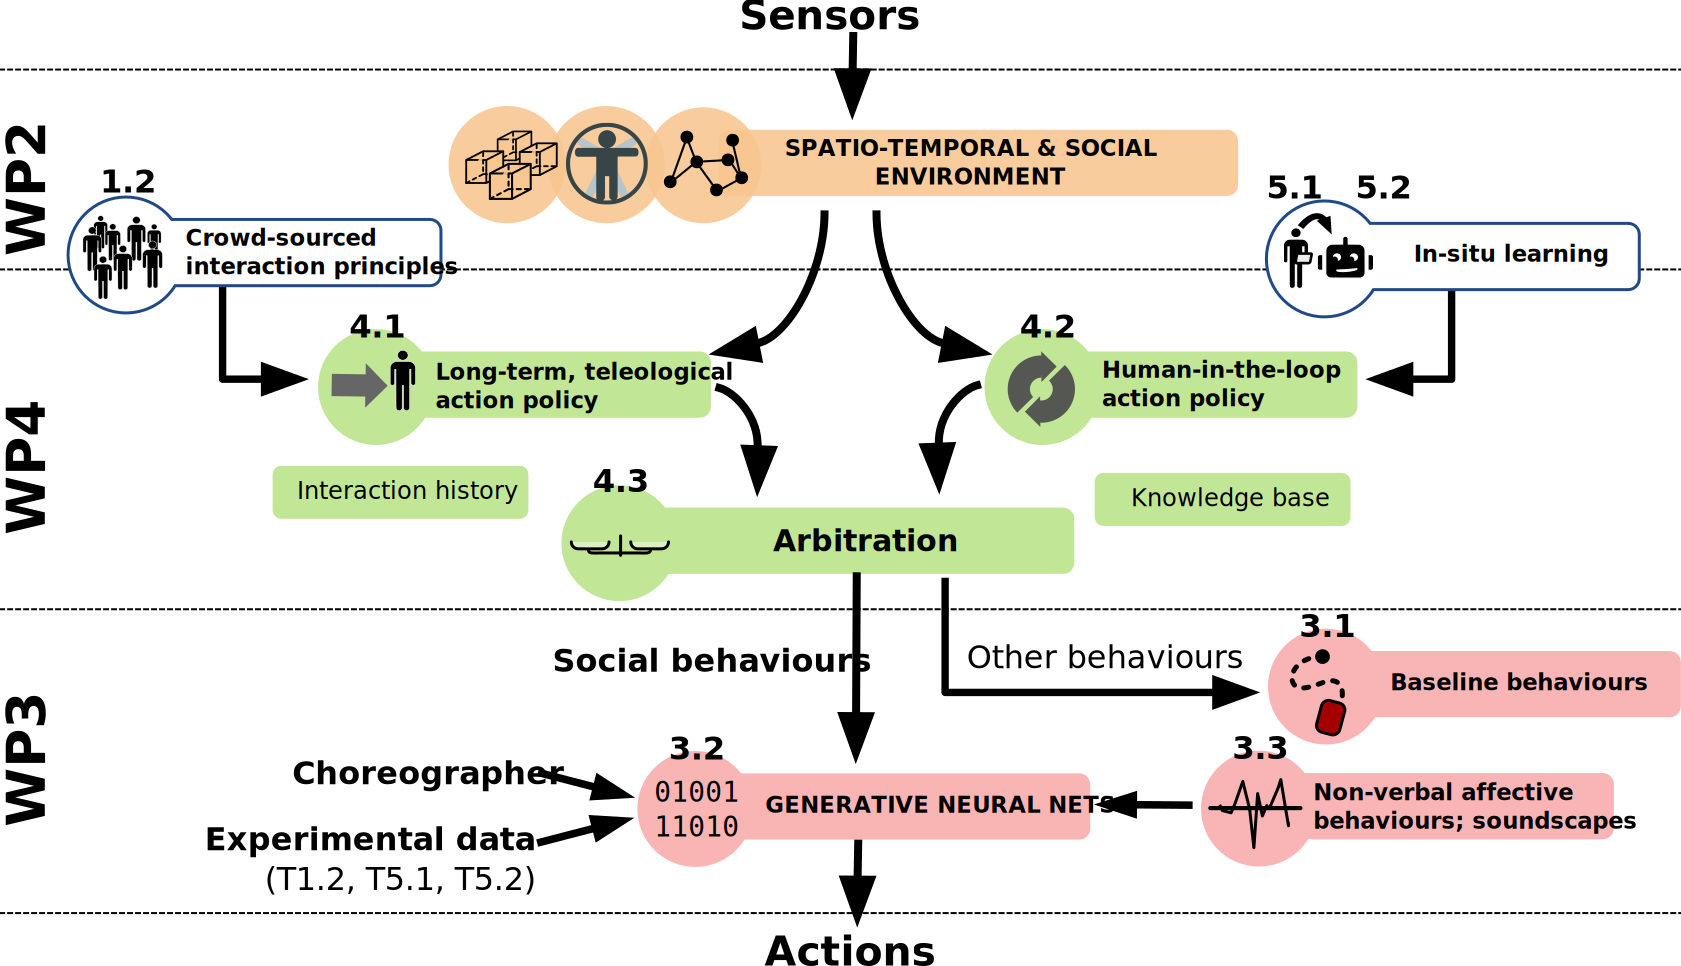
\includegraphics[width=0.9\linewidth]{figs/archi}
\caption{Overview of the technical architecture enabling social situation
    assessment: social situation assessment builds on strong \emph{situation
    assessment}, on top of which humans and human interactions are layered.}
\label{fig:social-situation-assessment}
\end{figure}



\subsection{T2.1}

 Beyond traditional
techniques like semantic scene segmentation, human skeleton tracking, speech
recognition, facial expression and gaze tracking, the robot will also be endowed
with novel capabilities to model the important social dynamics and interactions
taking place around the robot.


\subsection{T2.2}




%%%%%%%%%%%%%%%%%%%%%%%%%%%%%%%%%%%%%%%%%%%%%%%%%%%%%%%%%%%%%%%%%%%%%%%%%%%
%%%%%%%%%%%%%%%%%%%%%%%%%%%%%%%%%%%%%%%%%%%%%%%%%%%%%%%%%%%%%%%%%%%%%%%%%%%
\section{WP3: \wpThree{}}

\paragraph{Disembodied Cognitive Architectures}

Reviews: \cite{chong2007integrated}, \cite{vernon2007survey} --
extended in \cite{kingdon2008review}, \cite{duch2008cognitive},
\cite{langley2009cognitive}, \cite{taatgen2010past},
\cite{thorisson2012cognitive}.


\paragraph{Social Robotics Architectures}\label{sec:robots}


\emph{Society of Mind}-inspired paradigm underpinning practical architectures

Mostly functional architectures: integration models rather than cognitive
architectures per se.

\begin{figure}
    \centering

    \resizebox{\linewidth}{!}{%

        \tikzset{subpart/.style={draw, font=\scriptsize, fill opacity=0.5, text opacity=1, fill=white!50}}
    \begin{tikzpicture}[
            >=latex,
        every edge/.style={draw, very thick},
        skill/.style={draw, align=center, inner sep=5pt, fill=black!20},
        stmt/.style={align=center, font=\bf},
        label/.style={midway, align=center, font=\scriptsize, fill=white}]

        %%% Knowledge base
        \node at (0,0)[skill] (kb) {\bf Memory/Knowledge Base(s)\\ \footnotesize for instance, a symbolic blackboard};

        %%% Symbolic task planner
        \node at (-6, 2.5)[skill] (taskplanner) {{\bf Symbolic Task planner}\\ \footnotesize possibly human-aware};

        %%% Communication
        \node at (-6, -3) [skill] (communication) {{\bf Multi-modal communication}\\NLP, back-channel,...};

        %%% Abstract world model
        \node at (4,-3.5)[skill] (abstractenv) {%
            \begin{tikzpicture}
                \node at (0,0) (geom) {\bf Amodal Model of the Environment};
                \node [subpart, below=0.2 of geom.south west, anchor=north] (world-update) {Sensors fusion};
                \node [subpart, right=0.2 of world-update] (geom-model) {Situation assessment};
                \node [subpart, right=0.2 of geom-model] (fact-prod) {Temporal reasoning};
            \end{tikzpicture}
        };

        %%% Motion planner
        \node at (8.5,0)[skill] (motionplanner) {\bf Motion and manipulation \\ \bf planning};

        %%% Supervision
        \node at (4,4.5)[skill] (supervisor) {%
            \begin{tikzpicture}
                \node at (0,0) (exec) {\bf Supervisor};
                \node [subpart, below=0.2 of exec.south west, anchor=north west] (plans) {Goal \& Plans \\ management};
                \node [subpart, right=0.2 of plans] (sit-asses) {Context management};
                \node [subpart, right=0.2 of sit-asses] {Action instantiation, \\ execution and monitoring};
            \end{tikzpicture}
        };


        %%% LOWLEVEL
        \node [skill, below=0.7 of abstractenv,minimum width=6cm,minimum height=1.5cm,fill=black!30] (lowlevel) {\bf Sensorimotor layer};

        %%% Separation between deliberative layer and sensori-motor layer
        \draw[dotted, thick] (-8,-5) -- (12, -5);

        %%% Relations between components
        \path (supervisor.340) edge [<->, bend left] node[label] {motion plan \\ requests} (motionplanner);
        \path (supervisor.west) edge [<->, bend right] node[label] {plans} (taskplanner);
        \path (taskplanner) edge [<->, bend right] node[label] (domain) {world model and \\ agents beliefs} (kb.170);
        \path (communication) edge [<->, bend left] node[label] (nlp) {communication \\ grounding} (kb.190);
        \path (abstractenv.100) edge [->, bend right] node[label] (symfact) {abstract world\\ description} (kb);
        \path (abstractenv.5) edge [->, bend right] node[label] {geometric\\model} (motionplanner);
        \path (supervisor) edge [<->, bend left] node[label] (evts) {events, \\ world model and \\ agents beliefs} (kb);
        \path (lowlevel) edge [->] (abstractenv);
        \path (lowlevel.east) edge [<-, bend right=80, looseness=1.2] node[label] {atomic\\actions} (supervisor.east);

    \end{tikzpicture}
    }
    \caption{High-level representation of a typical \emph{practical} software
    architecture found in social human-robot interaction (based
    on~\cite{lemaignan2016artificial}). Arrows represent interfaces
    between independent software modules. They evidence the engineering
    perspective often favoured in robotic: cognition is seen as the result of a
    collection of individual cognitive skills, each implemented as an
    independent software component.}

    \label{fig:robot-archi}
\end{figure}

ACT-R/E~\cite{trafton2013act}, HAMMER~\cite{demiris2006hierarchical}, PEIS
Ecology~\cite{saffiotti2005peis,daoutis2012cooperative},
CRAM/KnowRob~\cite{beetz2010cram, tenorth2009knowrob},
KeJia~\cite{chen2010developing}


\paragraph{To be sorted...}

To check -- they may or may not be all relevant to sHRI.

Architectures that...

\begin{itemize}
    \item ...reason about other agent mental state
    \begin{itemize}
        \item Scone~\cite{fahlman2011using}
        \item Polyscheme~\cite{bello2011shared}
    \end{itemize}
    \item ...'represent knowledge'
        \begin{itemize}
            \item \cite{zhang2014towards}
        \end{itemize}
    \item ...cover the 'whole interaction stack'
        \begin{itemize}
            \item POETICON++ arch~\cite{antunes2016from} 
        \end{itemize}
\end{itemize}

\subsection{T3.2}

The current state-of-the-art is limited in this respect: sub-symbolic
approaches focus on identifying low-level social signals (for instance,
gazing, gesture recognition) while symbolic approaches have focused on
classical symbolic problems like language understanding. Some attempts
have been made to bridge both (for instance, multi-modal dialogue
\cite{lemaignan2011grounding, lemaignan2017artificial}), but no work to
date has been able to interpret the social dynamics themselves (for
instance, \emph{are the partners getting along well?}, \emph{Is there
any frustration?}, \emph{Are they collaborating or not?}, \emph{Are they
engaged in their joint task?}). This is likely due to the complexity of
the problem, mixing sub-symbolic and symbolic reasoning in intricate
ways. Understanding social dynamics in naturalistic conditions entails
identifying a complex net of overlapping social cues, at multiple time
scales. Reasoning about these ever-changing, sometimes contradictory,
dynamics, is an essential skill for an artificial socio-cognitive
system, yet an essentially open research question.

I have recently introduced a dataset of social
interaction~\cite{lemaignan2018pinsoro} that enables for the first time a
quantitative, data-driven investigation of social dynamics. Promising initial
results led me to uncover three latent constructs that underpin social
interactions~\cite{bartlett2019what}. This dataset and the related on-going
scientific investigations will form the starting point of my approach to this
challenge.


%%%%%%%%%%%%%%%%%%%%%%%%%%%%%%%%%%%%%%%%%%%%%%%%%%%%%%%%%%%%%%%%%%%%%%%%%%%
%%%%%%%%%%%%%%%%%%%%%%%%%%%%%%%%%%%%%%%%%%%%%%%%%%%%%%%%%%%%%%%%%%%%%%%%%%%
\section{WP4: \wpFour{}}
\subsection{T4.2: Machine learning for continuous motion generation}

\begin{wrapfigure}{l}{7cm}
    \centering
    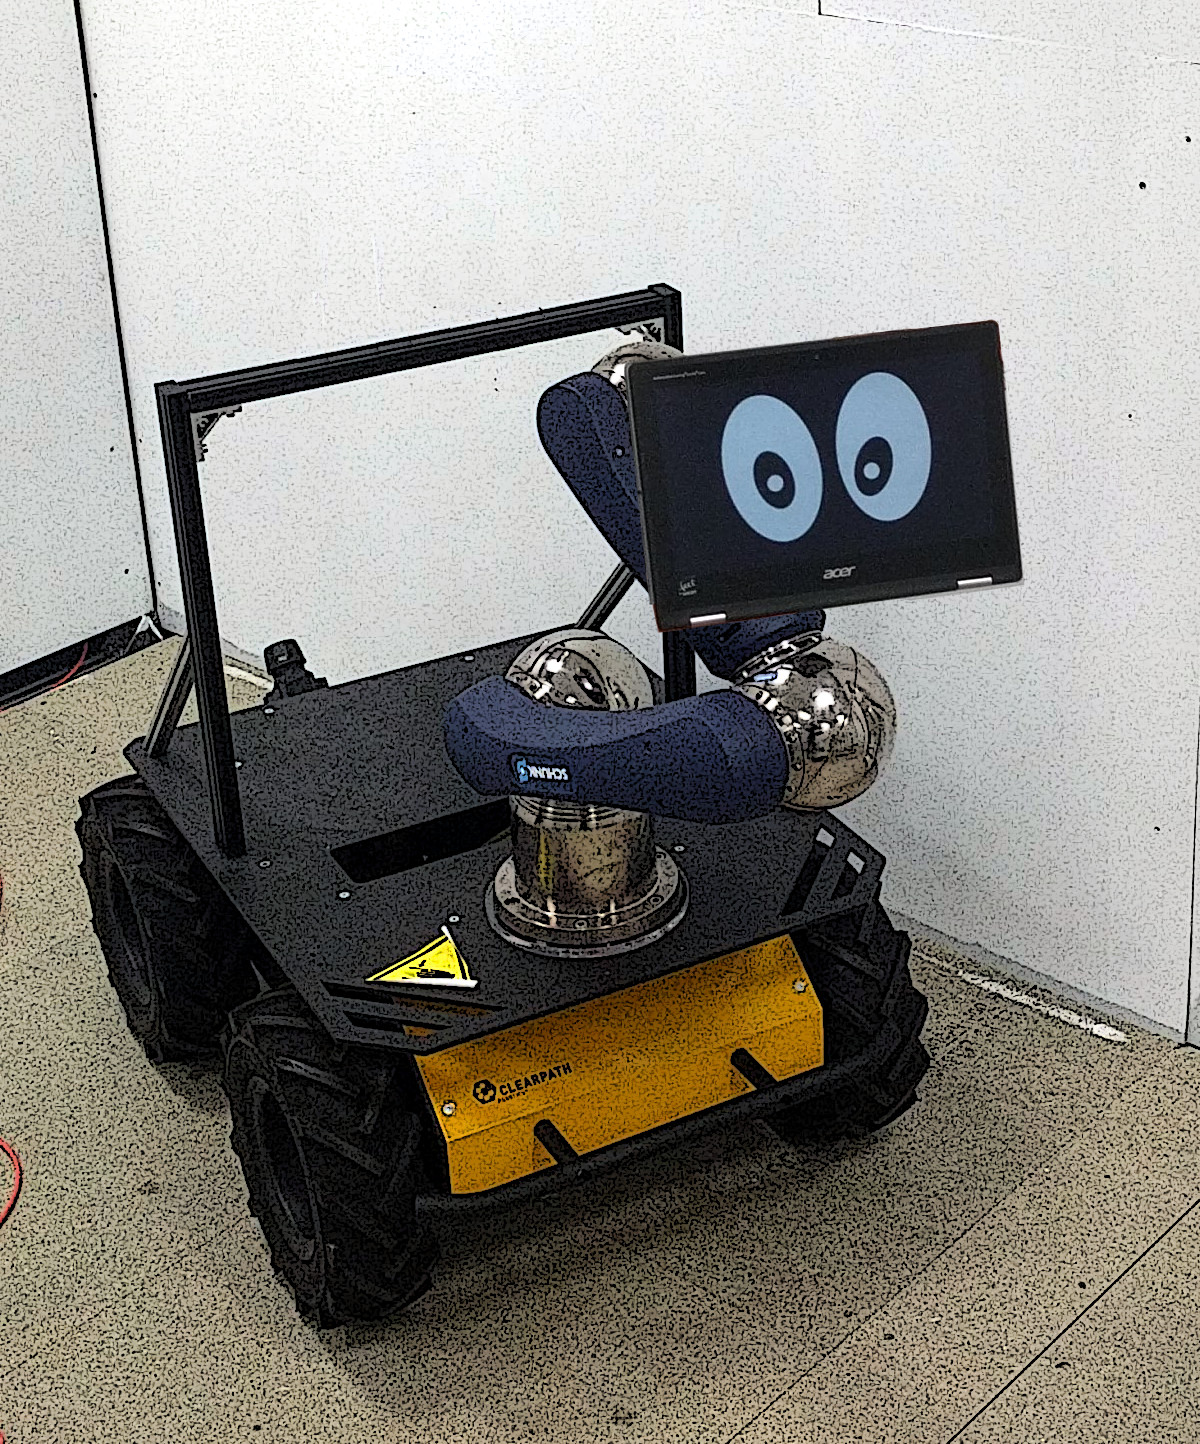
\includegraphics[width=\linewidth]{figs/husky.jpg}
    \caption{\label{fig:robot}
    Provisional appearance of the \project robot that we will use to collect
    data. A tablet, displaying facial animations, is mounted on a robotic arm.
    It can freely orient its `gaze' and use expressive movements. The mobile
    base (a Segway Husky) can autonomously navigate in the various parts of the
    BRL open-space}
\end{wrapfigure}

Designing behaviours that
enable sustained, long-term engagement in a social human-robot interaction is
essentially an open research question. Three main approaches to social
behaviours generation exist today: \emph{user-induced}, where the end-user
interacts with the robot and ascribes (knowingly or not) complex behaviours to
the machine, while in reality the robot's behaviours are simple and non-goal
oriented (eg generating a noise or a small movement when being touched). This
has been used to great effect in therapy robots, for instance (eg Paro).
\emph{Off-the-shelf behaviours}, where the robot relies on a set library of
behaviours (that might be individually relatively complex). The approach can
elicit a strong initial social response from the user, but this social response
tends to vanish rapidly once the 'tricks' of the robot have been all discovered
and become repetitive.  Besides, as the robot does not typically maintain a
long-term socio-cognitive plan of the interaction, the behaviours are typically
perceived as fun, yet pointless. This is often observed in toy-like robots (eg
Vector, Dot \& Dash). Finally, many social robots avoid altogether the problem
of generating behaviours by simply offering to the end-user control over
\emph{low-level behaviours} (eg, control of the joints of the robot). This means
that, even when the robot has relatively powerful social perception capabilities
(like recognising people and voice), no real social behaviours is generated.

None of these three approach is satisfactory, and indeed, no approach to date
has been able to engage human users in long-term, sustained interactions.




At a time where companion robots are coming to the market, one important
question remains fully open: how to design robot behaviours that foster
lasting engagement? A vast body of academic literature identifies that
robots evoke an initial phase of high user engagement (the
\emph{novelty} phase) that vanishes as the user realises that the robot
is actually quite predictable and repetitive. The \emph{agency}
initially ascribed by the user to the robot quickly
fades~\cite{lemaignan2014dynamics}, leading to critical user disengagement from the technology.


The (often limited) library of behaviours available to the robot is
often cited as a key factor in causing this issue. However, another,
more profound issue affecting long term engagement with robot companions
is the question of \emph{purpose.} Without clear \emph{purpose}, social
robot companions can lack \emph{usefulness}. Indeed, robot
\emph{companions} might not have explicit goals that would dictate or
motivate their behaviours: they aim at providing a social presence, a
social comfort, as cats or dogs would do, without necessarily being
goal-oriented.

Recent attempts -- and failures -- to convert social robotics research
into commercial platforms (Jibo, Kuri and most recently Anki's Cozmo and
Vector robots) reflect exactly this, with reasons for their failure
typically citing an under-delivery of the user experience they promised,
and/or the lack of a `real need' to justify their price point. The
\project project addresses these two key issues by:

\begin{enumerate}
\def\labelenumi{\arabic{enumi}.}
\item
  Taking inspiration from human-pet relationships which also have no
  explicit \emph{purpose} beyond their potential for enjoyable,
  \emph{affective} interactions;
\item
  Working with creative professionals who excel at storytelling and
  emotional engagement to overcome the problems in sustaining
  engagement, as proposed by Hoffman\footnote{\url{https://spectrum.ieee.org/automaton/robotics/home-robots/anki-jibo-and-kuri-what-we-can-learn-from-social-robotics-failures}};
\item
  Blending these two sources of inspiration using a radically novel
  combination of immersive teleoperation and machine learning.
\end{enumerate}

The project is \emph{not} about replicating a pet's behaviour per se. It
is instead about identifying, modeling and automatically generating the
social behaviours required to recreate pet-like social dynamics between
robots and humans, drawing inspiration from ethology (Stanton, Sullivan,
and Fazio 2015). Using animal behaviours to inform the design of robots
is not new, the most remarkable example being the Sony AIBO robot dog,
whose behaviours were directly designed around those of actual dogs
(Arkin et al. 2003). However, to go beyond the repetitive interactions
associated with such robots, we propose to employ a creative
professional to actively participate in design and automation of \project
behaviour. The concept of using creative professionals to `teach' social
robot behaviour is not new either (Knight and Gray 2012), however it is
only recent advances in human-in-the-loop, online machine learning that
make this type of real-time `social training' a feasible approach to
generating and automating engaging social behaviours (Senft et al.
2019).

Our project has the following goals, addressed by the workplan presented
below:

\begin{enumerate}
\def\labelenumi{\arabic{enumi}.}
\item
  assemble a non-anthropomorphic social robot that can autonomously
  navigate in a complex and living lab environment, taking inspiration
  from ethology to inspire the robot's behaviour;
\item
  develop an immersive teleoperation system, enabling a creative
  professional to `take control' of the robot (i.e.~puppet the robot) in
  a completely intuitive way (using whole body motion tracking);
\item
  record (and make publicly available) a large dataset of social
  behaviours (created through immersive teleoperation) that foster
  long-term social and affective engagement. The dataset will also
  include the social \emph{signals} implicitly used by the puppeteer to
  drive his/her choice of actions (recorded through eg eye-tracking);
\item
  using machine learning, map these social signals (input state) to the
  robot behaviours (output state) such that the robot can operate
  autonomously.
\end{enumerate}

A creative professional (puppeteer, dancer or comedian --
corresponding financial compensation is budgeted) will join the group.
First she/he will take part to a one-week co-design workshop (4) aiming
at finalising the immersive teleoperation controller and the behaviours
of the robot. Then, she/he will interact for about 4 hours a day during
a month, with the BRL lab members (200+ researchers). She/he will do so
by remotely operating the robot (5) from an (out-of-sight) control room
(the BRL CAVE room). The aim will be for the puppeteer to pro-actively
engage with people in the lab, attempting to engage in \emph{social,
affective} interactions. This will be achieved by creating/inventing
in-situ a new `grammar' of social behaviour, loosely inspired by those
of cats and other pets. These interactions will be fully recorded
(including eye-tracking on the puppeeter) (6), in order to create a
unique dataset of complex social interactions, suitable for machine
learning. The PI has already extensive experience in recording such
datasets (see (Lemaignan et al. 2018) for instance).

%\begin{wrapfigure}[17]{l}{8cm}
\begin{figure}
    \centering
    
\includegraphics[width=0.8\paperwidth]{figs/dev.pdf}
    \caption{\label{fig:support}
    Social behaviours will be learned from immersive `puppetering' of the
    robot, performed by a professional actor. The `puppetering' takes place
    in a CAVE (or VR) environment, where what the robot `sees' and `hears'
    is streamed live}
\end{figure}
%\end{wrapfigure}

Over the following four months, a deep neural network will be designed
and trained (7) for the regression task of generating continuous social
behaviours from perceived social signals. In parallel, a software
controller will be developed (8) to enable generic autonomous
capabilities (like autonomous navigation) for which the BRL has
extensive expertise.

Finally, the last four months will be dedicated to in-situ testing of
the autonomous system (9). We will seek to conduct a large scale study
within the lab, over a period of several weeks. For this study, the
robot is expected to be fully autonomous. However sufficient amount of
time is planned for additional iterations on the development of the
robot controller if deemed necessary. We aim at publishing the results
of this main study shortly after the end of the one-year period.


\subsection{T4.3: Non-verbal behaviours and robot soundscape}

\begin{figure}[!htbp]
\centering
    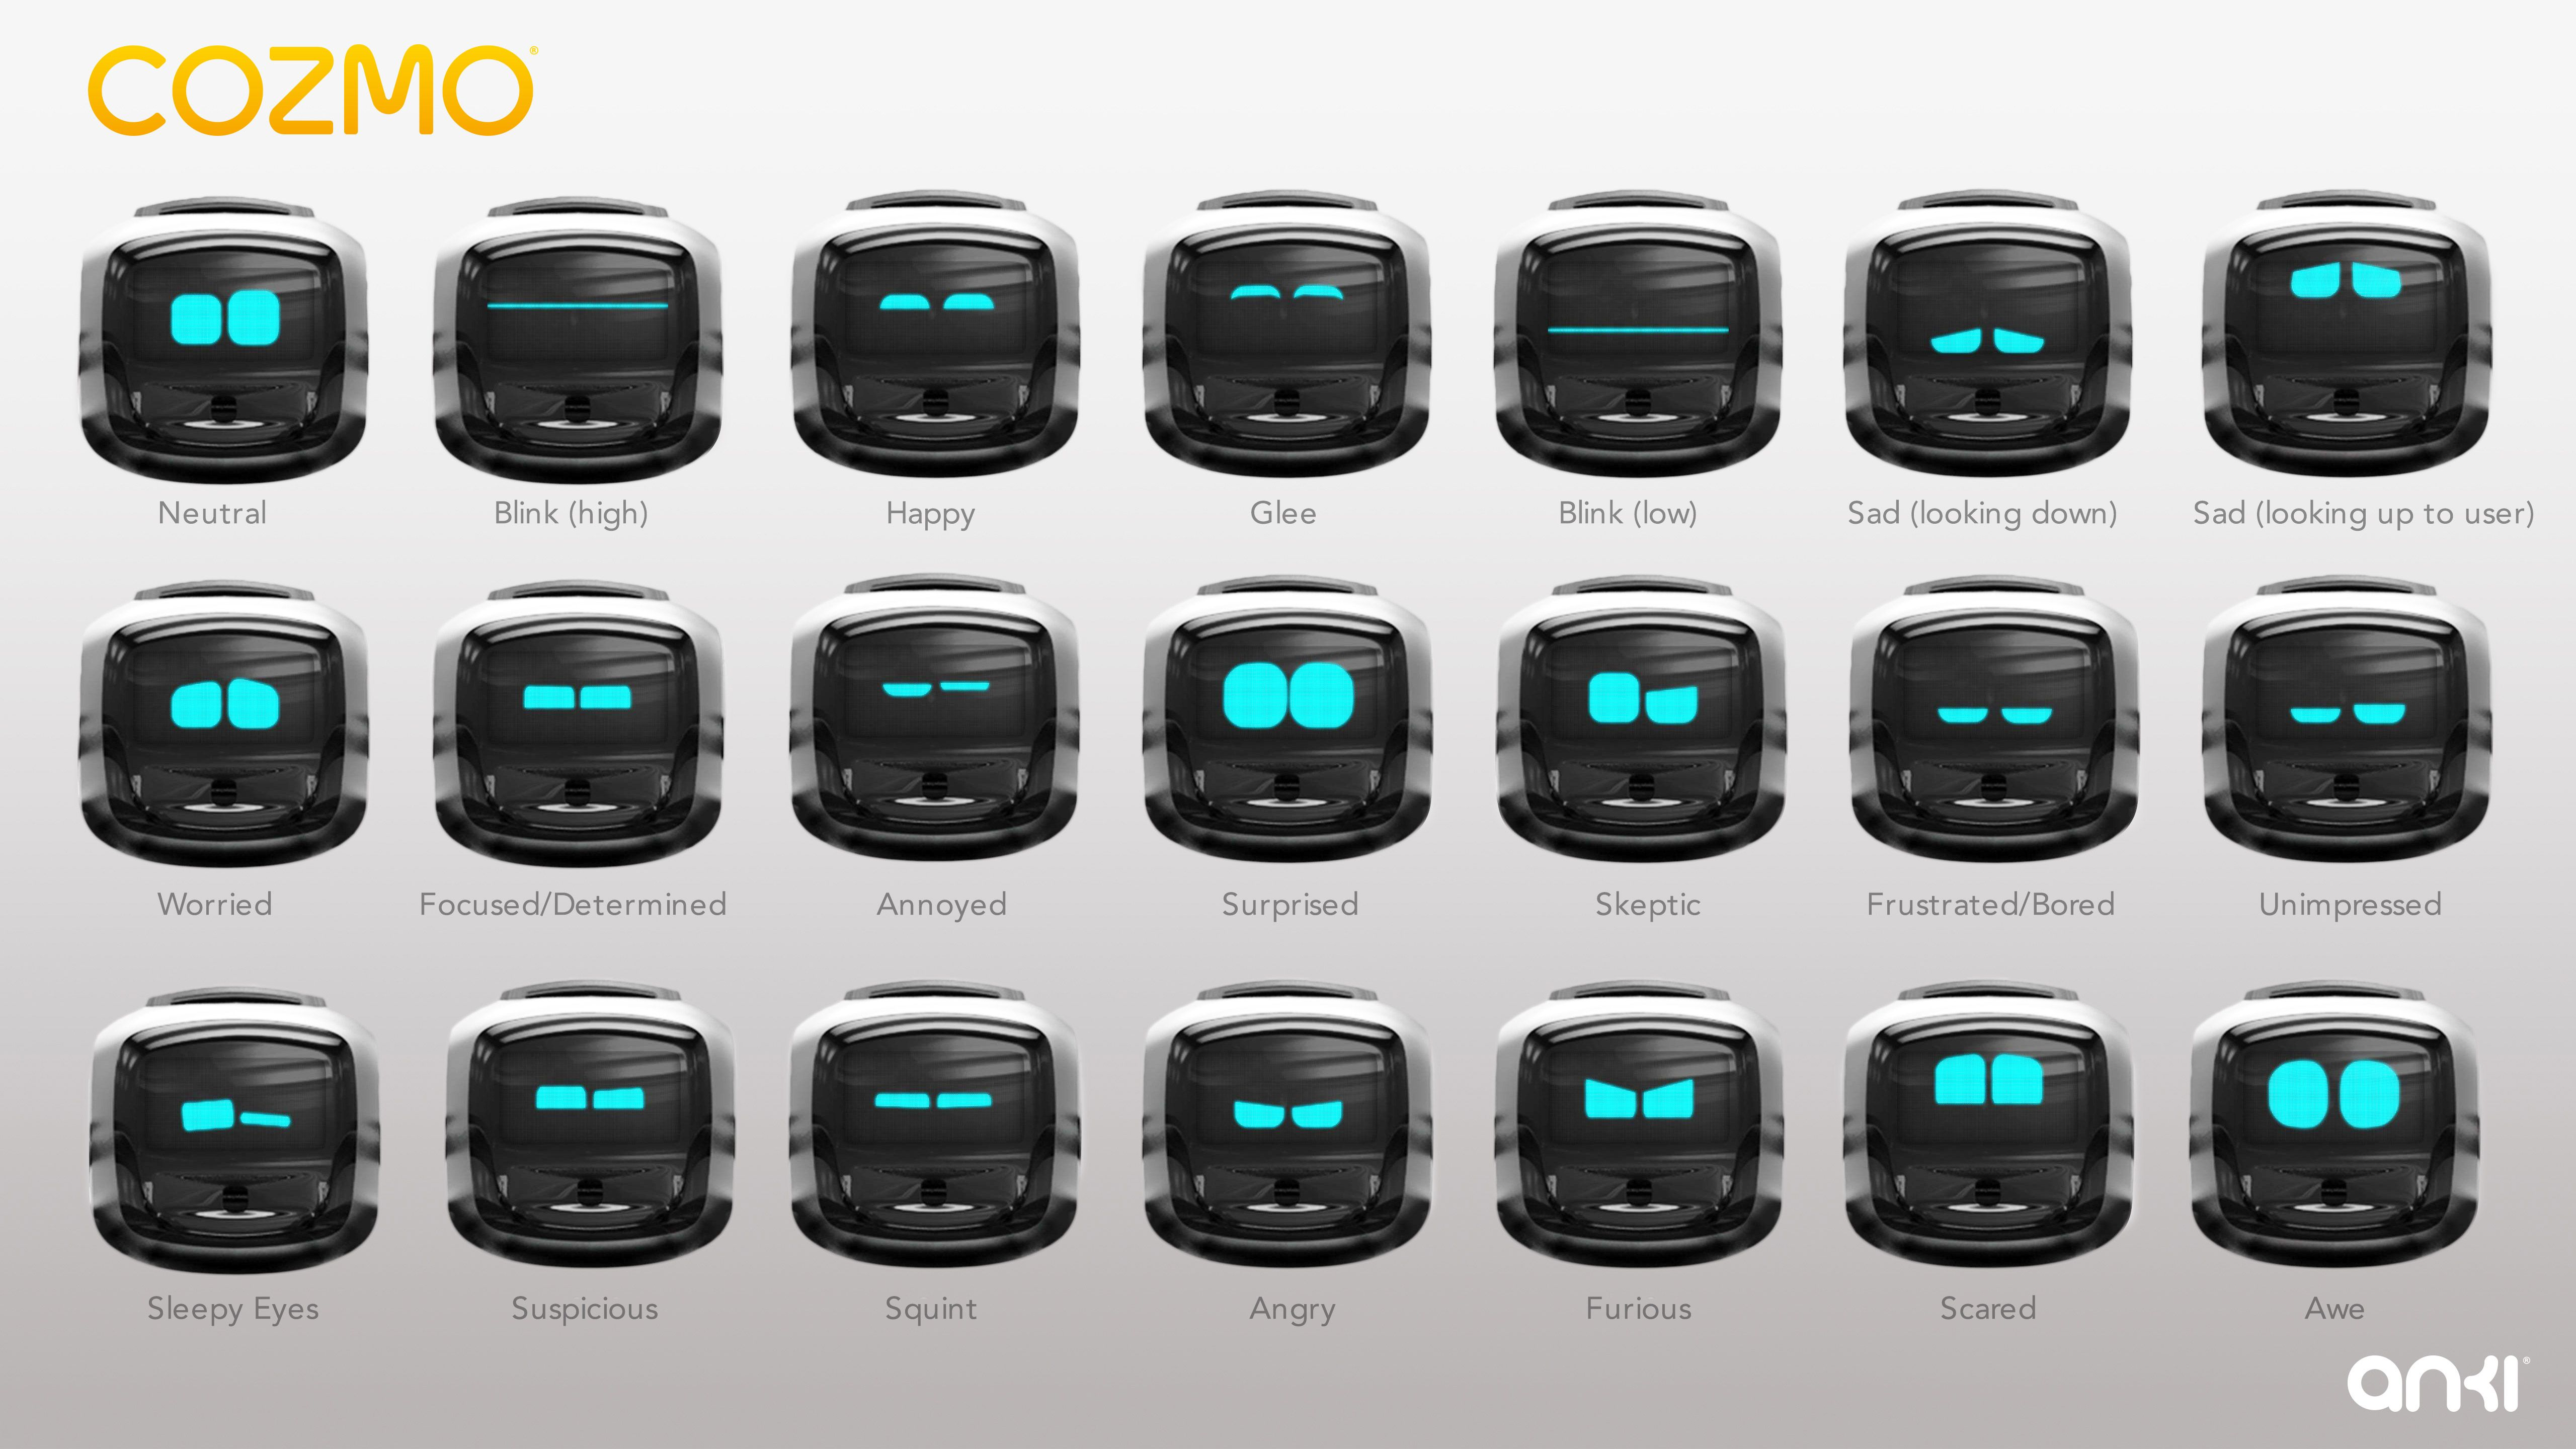
\includegraphics[width=0.7\textwidth]{figs/cozmo-expression-sheet.jpg}
\caption{Cozmo facial expressions}
\end{figure}



\section{WP5: \wpFive{}}


%%%%%%%%%%%%%%%%%%%%%%%%%%%%%%%%%%%%%%%%%%%%%%%%%%%%%%%%%%%%%%%%%%%%%%%%%%%
\subsection{Evidence-based research: demonstrable usefulness of social robots in
real-world, complex scenarios}


Critically, the scientific investigation of these questions (\emph{conceptual
framing of robot-supported human-human interaction}, \emph{socially-driven
cognitive architecture},  \emph{online social situation assessment and social
behaviour generation}) has to be
grounded in real-world applications. Indeed, two complex, high impact
applications are detailed in the project. The first one takes place in
Bristol's Children Hospital: a social robot will be permanently deployed in one
of ward, supporting isolated children who suffer long-term conditions, in close
cooperation with the hospital staff. The second one involves the deployment of 
social robots in special need schools (SEN schools) in Bristol. Building on a
rigorous participatory approach involving the school teachers, as well as the
parents, we will seek to integrate the robot in the daily life of the school,
supporting the development of the students' physical and social skills.

These two applications, detailed hereafter, aim at supporting
socially-vulnerable populations: this entails specific risks (detailed and
addressed in the Section~\ref{risks}), but also offers a unique opportunity to
demonstrate in a real-world, impactful case, how social robots can effectively
have a positive, ethical impact, and support in-fine stronger, richer
human-human interactions.


\project aims at developing and demonstrating the need for a global approach to
social HRI with ambitious, high-impact, socially meaningful, applications.

The two last application scenarios are ambitious and inherently risky, as they
target vulnerable populations. This is an however informed choice: first, we
already have established partnerships with Bristol's children hospital on one
hand, and a network of Bristol-based SEN schools on the other hand. As such, and
from a practical perspective, we do not foresee any institutional issues -- on
the contrary, our partners are excited at the prospect of taking part to the
project. Besides, convincingly demonstrating the importance and positive impact
of socially-driven, socially-responsible robotics does accordingly require
complex social situations, and complex social dynamics. The two scenarios, which
complement each other, provide both. These scenarios also put the project in the
unique position of actually delivering high societal impact: we anticipate 100+
hospitalised children with long-term conditions, and 50+ SEN-educated children
to directly benefit of the project, showing how robots can have a lasting,
strong, positive impact on the society, also establishing the idea of
\emph{robots supporting human interactions} instead of dehumanising our social
relationships.


\TODO{probably useful to give specific examples of interventions}


\subsection{Application 1: Social robots in SEN schools}

Can a socially assistive robot effectively support the development (learning?),
social interactions and well-being of children with a long-term mental
condition? Our project aim is an investigation of this question: how can a
social robot integrate into the eco-system of a SEN (Special Educational Needs)
school (specifically, the Mendip School, which welcomes pupils with ASD
(Autistic Spectrum Disorder), and effectively support the day-to-day work of the
school staff to support the development, learning and well-being of the
children. This project is naturally interdisciplinary as it requires expertise
from mental health/special needs education, classroom design and social
robotics. 

The main questions we seek to investigate are: What are the (social \& spatial)
underpinnings of the successful integration of a social robot in the school
ecosystem? Can ambitious co-design with the end-users (teachers) deliver a 'net
gain' for the learning, social interaction and well-being of the students? 


The core of the project consists of deploying a social robot (likely one of the
BRL-owned Softbank Peppers) in a Bristol-based SEN school (the Mendip School),
to investigate how the robot can help shaping a spatial and social school
ecology that fosters mental well-being, while effectively supporting teachers
and students in their learning. 

The project will adopt a strong participatory design approach, with 2 one-day
workshops organised with the school teachers; and one evening workshop with the
school parents, prior to the school study (Jun./Jul. 2020). During the first
workshop, the teachers will be introduced to the robot capabilities with
examples of robot-supported teaching activities, and the robot's visual
programming interface will be introduced. We will also conduct group discussions
on how the robot can best be integrated in the daily school routine and
classroom context. During the second workshop, the teachers will be invited to
create novel activities, with the support of the research team. An evening focus
group will be organised as well with the parents, to integrate their
perspectives in the design of the robotic system.  Will we formally analyse the
data from this – will it become a research paper? 

Following the workshops, the teacher-oriented codesign of the robot's activities
and supervision tools (eg to start/stop/pause/resume activities) will be
finalised and implemented by the research team (Aug./Sep.2020). 

The school study itself will take place over 2 months (tentatively Oct./Nov.
2020), with the robot visiting the school once a week for the whole day. During
these visits, the robot will take part in the regular teaching and other daily
routines of the school, and will directly interact with the children. While the
robot's behaviours will have been co-designed with the teachers, the robot will
be teleoperated by a member of the research team, to ensure we do not create an
additional burden for the staff. 

During the 'robot days', observations will be conducted by the research team,
and regular semi-structured interviews will be conducted with the teachers,
parents, and where possible, the children themselves, to understand how the
robot impacts the school dynamics  (both positively and potentially negatively).
Is it appropriate/pertinent to do pre- and post- surveys of acceptance of robot? 



\subsection{Application 2: A robot companion at the children's hospital}


\TODO{explain that these 2 large experiments will be scaffolded by many smaller
ones}

\subsection{Experimental deployments: risks and mitigations}

These two application scenarios are ambitious and inherently risky, as they
target vulnerable populations. However, first, demonstrating the
importance of advanced social modelling, and convincingly proving the
effectiveness of our approach does require accordingly complex social
situations, and complex social dynamics. The two scenarios, which complement
each other, provide both.

Second, working with vulnerable populations, in constrained and complex
environments (children hospital and SEN schools) adds significant risks to the
project. But it is also what make the project in the unique position of
delivering a high societal impact: a direct positive impact on children's
lives (we anticipate 100+ hospitalised children and 50+ refugee children
interacting over long periods of time with a robot over the course of the
project), and a broader impact on the society, showing how robots can have a
lasting, strong, positive impact on the society, also establishing the idea of
\emph{robots supporting human interactions} instead of dehumanising our social
relationships.

The two main mitigations are (1) early and continuous engagement with the
stakeholders, and (2) the decoupling of the two applications, meaning that the
risks associated to each of them do not impact the other one.

Early engagement will be ensured by relying on a participatory design
methodology, involving all the stakeholders from the onset of the project; the
methodology will involve regular joint workshops; on-site (hospital and refugee
camps) research stay including engagement with the staff/charities and the
children themselves; use of art-based participatory techniques like puppetering.
I will also perform field testing early on in the project, relying if necessary
on provisional robot platforms available at the host institution (for instance,
Softbank Nao and Pepper). This user-centered approach will be championed by one
of the post-doc recruited on the project, who will have recognised expertise in
user-centered design.


The Principal Investigator, Dr.  Séverin Lemaignan, has been working for 12+
years in human-robot interaction, and over the last 6 years, specifically in the
field of child-robot interaction.  His profile is both highly technical, with
hundreds of hardware and software contributions to the worldwide robotic
community; and highly experimental, running dozens of studies and experiments
with children, including long-term ones, in muliple schools and in healthcare
environments. He is in a unique position to deliver both a scientific
breakthrough on social situation assessment for robots, and a high-impact
societal change.

%%%%%%%%%%%%%%%%%%%%%%%%%%%%%%%%%%%%%%%%%%%%%%%%%%%%%%%%%%%%%%%%%%%%%%%%%%%
%%%%%%%%%%%%%%%%%%%%%%%%%%%%%%%%%%%%%%%%%%%%%%%%%%%%%%%%%%%%%%%%%%%%%%%%%%%
\section{Interdisciplinarity}


\section{Responsible Research and Innovation (RRI)}



One example: a common (ethics-related) objection to human-robot interaction is
the perceived deceptive nature of the robot's role. As recently
argued~\cite{biscontilucidi2018companion}, the underlying concern is likely
instead the need to simulate of a human-like interaction with robots, in the
absence of an adequate (and novel) model of human-robot interactions to refer
to.


BS 8611~\cite{bsi2016robots}
~\cite{stahl2018implementing}


\TODO{taken from Stahl2018; rephrase}

The EC has adopted RRI as a cross-cut-
ting activity in its Horizon 2020 research framework programme.

For the purposes of this paper, I will use the concept of RRI as put developed
by~\cite{stilgoe2013developing} and subsequently adopted by the UK Engineering
and Physical Sciences Research Council~\cite{owen2014uk}. This concept
represents RRI using the acronym AREA, which stands for anticipation,
reflection, engagement and action. A piece of research or innovation activity,
in order to count as having been undertaken responsibly, would need to
incorporate anticipation about possible consequences, integrate mechanisms of
reflection about the work, its aims and purposes, engage with relevant
stakeholders and guid action of researchers accordingly.

AREA 4P
Framework~\cite{stahl2018implementing}~\footnote{\url{https://www.orbit-rri.org/about/area-4p-framework/}}


%%%%%%%%%%%%%%%%%%%%%%%%%%%%%%%%%%%%%%%%%%%%%%%%%%%%%%%%%%%%%%%%%%%%%%%%%%%%%%%%%%%%%%%%
%%%%%%%%%%%%%%%%%%%%%%%%%%%%%%%%%%%%%%%%%%%%%%%%%%%%%%%%%%%%%%%%%%%%%%%%%%%%%%%%%%%%%%%%
%%%%%%%%%%%%%%%%%%%%%%%%%%%%%%%%%%%%%%%%%%%%%%%%%%%%%%%%%%%%%%%%%%%%%%%%%%%%%%%%%%%%%%%%

\section{Risks}\label{risks}

\begin{table}[!htbp]
\caption{Identified risks and proposed mitigations}
\centering
\begin{tabular}{@{}lll@{}}
\toprule
\textbf{Description of risk} & \textbf{Work package(s) involved} & \textbf{Proposed risk mitigation measures} \\ \midrule
risk 1 (low/medium/high)     &                                   &                                            \\
                             &                                   &                                            \\
                             &                                   &                                            \\
                             &                                   &                                            \\ \bottomrule
\end{tabular}
\end{table}



%%%%%%%%%%%%%%%%%%%%%%%%%%%%%%%%%%%%%%%%%%%%%%%%%%%%%%%%%%%%%%%%%%%%%%%%%%%%%%%%%%%%%%%%
%%%%%%%%%%%%%%%%%%%%%%%%%%%%%%%%%%%%%%%%%%%%%%%%%%%%%%%%%%%%%%%%%%%%%%%%%%%%%%%%%%%%%%%%
%%%%%%%%%%%%%%%%%%%%%%%%%%%%%%%%%%%%%%%%%%%%%%%%%%%%%%%%%%%%%%%%%%%%%%%%%%%%%%%%%%%%%%%%


\newpage
\printbibliography

\newrefsection
\newpage
\chapter{B2.c Description of resources}

\eu{Has to be provided online; 8000 chars max (eg 2 pages)}


\section{Requested budget}

\TODO{This table does not count toward the page limit and is to be provided online}
\begin{table}[]
\begin{tabular}{@{}lll@{}}
\toprule
\textbf{Labour cost}                                             & \textbf{} & \textbf{€ 1,413,344} \\ \midrule
Severin Lemaignan                                                & 36        & € 287,455            \\
RF 1 (sociology/anthropology, WP1)                               & 36        & € 195,779            \\
RF 2 (social signal processing/machine learning, WP2)            & 48        & € 263,722            \\
RF 3 (cognitive architecture for robotics, experiments, WP3 WP5) & 60        & € 333,050            \\
PhD 1 (social signal processing/machine learning, WP3 WP5)       & 42        & € 64,233             \\
RF 4 (behaviour generation, WP4)                                 & 48        & € 269,105            \\
                                                                 &           &                      \\
\textbf{Travel}                                                  & \textbf{} & \textbf{€ 65,865}    \\ \midrule
Conferences (1 per person per year): Registration                &           & € 22,910             \\
Conferences (1 per person per year): Travel                      &           & € 42,955             \\
                                                                 &           &                      \\
\textbf{Equipment}                                               & \textbf{} & \textbf{€ 334,527}   \\ \midrule
R1 Robot (inc VAT)                                               &           & € 292,800            \\
R1 Shipping                                                      &           & € 7,000              \\
Robot Installation and Training                                  &           & € 3,800              \\
Workstation suitable for machine learning                        &           & € 22,910             \\
Sensors (inc RGB-D cameras, one eye tracker)                     &           & € 8,018              \\
                                                                 &           &                      \\
\textbf{Materials}                                               & \textbf{} & \textbf{€ 11,455}    \\ \midrule
Other Consumables                                                &           & € 11,455             \\
                                                                 &           &                      \\
\textbf{Other}                                                   & \textbf{} & \textbf{€ 23,455}    \\ \midrule
Open access fees (2 Article per year)                            &           & € 12,000             \\
Participants compensations                                       &           & € 3,436              \\
Data Storage                                                     &           & € 2,291              \\
Cloud Computing                                                  &           & € 5,727              \\
                                                                 &           &                      \\
Audit                                                            &           & € 5,000              \\
                                                                 &           &                      \\
                                                                 &           &                      \\ \midrule
\textbf{Total}                                                   & \textbf{} & \textbf{€ 1,853,645} \\
\textbf{Indirect}                                                & \textbf{} & \textbf{€ 463,411}   \\
\textbf{EC Contribution}                                         & \textbf{} & \textbf{€ 2,317,056} \\ \bottomrule
\end{tabular}
\end{table}

\section{Research team and PI commitment}

Table~\ref{time-allocation-team} provides an overview of the time allocation per
members of the team, over the course of the project.

\begin{table}[h!]
    \centering
\begin{tabular}{@{}lccccccr@{}}
\toprule
\textit{\textbf{}}              & \textbf{Y1} & \textbf{Y2} & \textbf{Y3} & \textbf{Y4} & \textbf{Y5} &  & \textbf{Total months} \\ \midrule
\textit{Séverin Lemaignan (PI)} & 0.6         & 0.6         & 0.6         & 0.6    & 0.6         &  & 36                    \\ \midrule
\textit{Post-doc 1 (WP1)}       & 1           & 1           & 1           &             &             &  & 36                    \\
\textit{Post-doc 2 (WP2)}       & 1           & 1           & 1           & 1           &             &  & 48                    \\
\textit{Post-doc 3 (WP3, WP5)}  & 1           & 1           & 1           & 1           & 1           &  & 60                    \\
\textit{PhD 1 (WP3, WP5)}       &             & 1           & 1           & 1           & 0.5         &  & 42                    \\
\textit{Post-doc 4 (WP4)}       &             & 1           & 1           & 1           & 1           &  & 48                    \\ \bottomrule
\end{tabular}
    \caption{Full-time equivalent for the research team members}
    \label{time-allocation-team}
\end{table}

PI Séverin Lemaignan will dedicate 60\% (3 days/week) of his time to the
project. This time will cover significant research time (about 2 days/week) as
well as the supervision of the team and management of the project (1 day/week).

The rest of his time will be dedicate to other academic commitments within the
Bristol Robotics Lab (including the on-going supervision of his other PhD
students, supervision of MSc students, the supervision of the Human-Robot
Interaction research group at BRL, lab-wide strategic engagement), as well as a
small proportion of Master-level teaching in Human-Robot Interaction (about 5
days/term).

Each of the project work packages will have one lead researcher (senior
post-doc); the duration of each of the post-docs' contracts roughly matches the
duration of the corresponding work packages.

\begin{itemize}
    \item \textbf{WP1}: I will appoint a post-doc with a background in sociology
        of technology and science facilitation; the researcher will work for
        three year to frame the \emph{robot-supported human-human interactions}
        paradigm, and lead the field work at the WeTheCurious museum;

    \item \textbf{WP2}: WP2 will be led by a post-doc with a background in
        social signal processing and/or machine learning; the researcher will be
        appointed for 4 years; extensive collaboration with WP1's post-doc is
        expected to frame the social dynamics fostered by the robot;

    \item \textbf{WP3}: WP3 (the cognitive architecture) lays at the core of the
        project; the WP3 leader will be a senior post-doc in cognitive robotics,
        appointed for the whole 5 years to ensure continuity on this critical
        part; she/he will be responsible for the integration of the outputs of
        the other work packages; the same post-doc will also oversee (with the
        PI) the experimental work taking place in WP5. A PhD student will also
        be recruited on WP3, with a specific focus on the cognitive architecture
        design;

    \item \textbf{WP4}: one post-doc (background in learning from demonstration
        and machine learning) will be in charge of developing the novel
        continuous robot behaviour generation method, and will be appointed for
        4 years, starting on the second year.

\end{itemize}
\section{Research equipement}

I will purchase 2 R1 robots for the \project project. The R1 robot is a
recently developped service robot from the Italian Institute of Technology
(IIT). Figure~\ref{r1-specs} summarises the main features of the robot.

While the host institution (the Bristol Robotics Lab) could provide access to a
range of social robots, none of the currently available robots are suitable for
the project.  Table~\ref{robot-comparison} compares the main R1's feature with
those of PAL TiaGo and SoftBank Pepper, the two main other platforms that would
be potentially suitable for the project. However, neither TiaGo nor Pepper have
non-verbal social features that are powerful enough to deliver the \project
project. Critically, they both lack the abilities to show facial expressions or
simulated gazing behaviours. Because the R1 robot features a programmable
display in place of the head, we will have full freedom to create complex
non-verbal facial expressions.

\begin{table}[]
    \begin{tabular}{@{}p{3cm}p{5cm}p{5cm}p{5cm}@{}}
\toprule
                                           & PAL TiaGo                                                & Softbank Pepper                                                           & \textbf{IIT R1}                                                                                                                              \\ \midrule
\textbf{Social features}                   & Poor (non-expressive head)                               & Medium (expressive, yet fixed, face; no gaze; non-threatening appearance) & Good (expressive face~\cite{lehman2016head}; artificial skin for touch-based interactions; non-threatening appearance) \\
\textbf{Perception}                        & Medium (RGB-D camera; laser scanner; no microphone)      & Medium (RGB-D; simple mic array; poor laser scanner)                      & \TODO{check once datasheet}                                                                                                   \\
\textbf{Navigation}                        & Good (however, limited agility due to large footprint)   & Poor (weak localisation capabilities)                                     & \TODO{check once datasheet}                                                                                                   \\
\textbf{Safety}                            & Medium (heavy robot; large footprint; non-compliant arm) & Medium (smaller footprint; safe arms; limited stability)                  & Good (smaller footprint; safe arms; dynamic stability)                                                                                       \\
\textbf{Suitability for care environments} & Poor (relatively large, difficult to clear)              & Good (smaller footprint, easy to clean)                                   & Good (smaller footprint, easy to clean)                                                                                                      \\
\textbf{Manipulation capabilities}         & Medium (non-anthropomorphic gripper; single arm)         & Limited (poor gripper with low payload; dual arm)                         & Good (anthropomorphic gripper; pressure sensors; dual arm; 1.5kg payload)                                                                    \\ \bottomrule
\end{tabular}
    \label{robot-comparison}
\end{table}

\section{Open access}

In line with the European requirements, all journal publications will made
available under an Open Access license. On the basis of an average of 2 journal
publications per annum, and an average processing fee of €1,200 per article, we
request €12,000 to support Open Access costs. Note that conference publications
do not always offer immediate open-access policies.

\section{Existing resources available to the researcher}

The fellowship will take place at the Bristol Robotics Laboratory (BRL).  The
BRL is the largest co-located and most comprehensive advanced robotics research
establishment in the UK. It is a joint venture between the University of the
West of England and the University of Bristol. BRL's multidisciplinary approach
aims to create autonomous devices capable of working independently, with each
other, or with humans. BRL draws on robotics, electrical \& mechanical
engineering, computer science, psychology, cognitive science and sociology. BRL
has an international reputation as a leading research centre in advanced
robotics research and has over 250 researchers working on a broad portfolio of
topics: HRI, collective robotics, aerial robotics, neuro-inspired control,
haptics, control systems, energy harvesting and self-sustaining systems,
rehabilitation robotics, soft robotics and biomedical systems. BRL has many
collaboration partnerships, both national and international, and is experienced
in managing large multi-site projects. BRL has support from two embedded units
specialising in business and enterprise, together with an incubator and
successful track record of spin-outs.

Hardware-wise, the Bristol Robotics Lab, where this fellowship will take place,
offer unique support and facilities for robotic hardware development: the
laboratory's dedicated equipment includes two industrial-grade rapid prototyping
machine, a laser cutter, one 5-axis digital milling machine, all the required
facilities for PCB prototyping, and a team of six full-time technicians,
specialised in hardware development. The BRL has indeed a long track-record of
designing and building new and original robots (from the BERT humanoid in the
FP7 CHRIS project, to micro-robotics [in...?], to [...]). \project will directly
benefit of this expertise, which will ensure a feasible and realistic technical
implementation of the \project robots. Besides, an hardware engineer, dedicated
to the project, will be recruited in the frame of the project.

The BRL also include a hardware incubator and is co-located with 70 start-ups
and SMEs specialising in robotic hardware and mechatronics (Bristol's
\emph{FutureSpace}). This combination of excellent research and vast industry
expertise on one site is unique in the UK, and is will play an instrumental role
in providing a coherent and strong pathway to impact to the project, including
further engagement with industrial partners and spin-off opportunities.


\printbibliography

\end{document}
